\chapter{Analysis of the Dynamic Performance of 2 GW, 66 kV HVAC Offshore Network}\label{5}

Connecting a large scale \gls{OWF} network to an offshore-onshore \gls{HVDC} link has always been a challenge. In this chapter, the operation scheme of the 2 GW offshore network presented in Chapter \ref{4} is simulated and analyzed. Firstly, the initial conditions of the converters are defined, and then the stage-wise synchronization and operation of the network is explained. Later, the network is tested for short-term voltage stability and the power flow analysis for severe disturbances such as sudden disconnection of one \gls{OWF} and a three-phase line to ground fault in the middle of a \gls{HVAC} cable.

\begin{figure}[H]
\centering
%\hspace*{-1.5cm}
    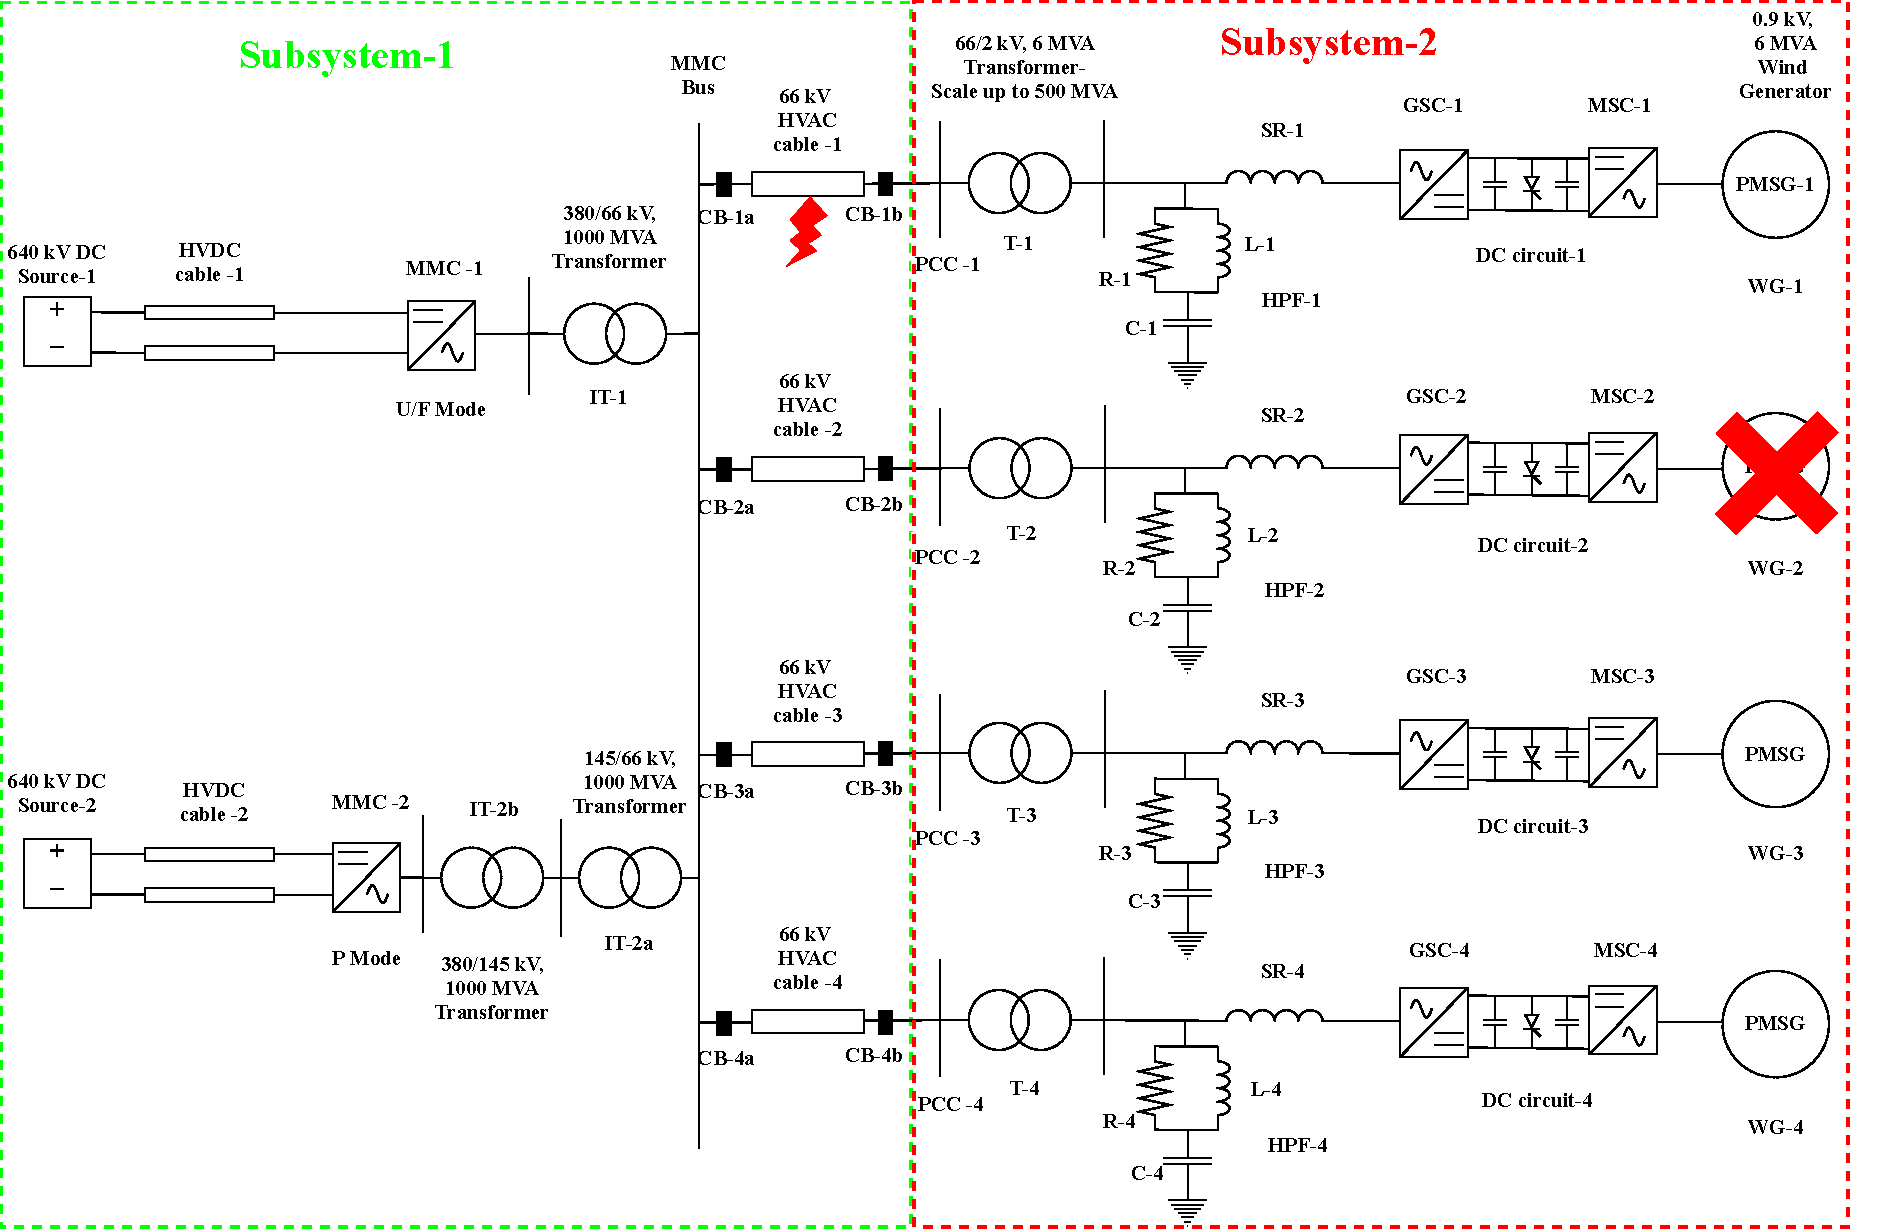
\includegraphics[height = 12cm,width = \textwidth]{Diagrams/Chapter_5/WT4_MMC2_fault.pdf}
    \caption{66 kV HVAC offshore network connected to 2 x 1 GW HVDC links with offshore converter stations in RSCAD for two dynamic scenarios- \newline 
    a) Disconnection of OWF-2 (represented by the cross symbol) \newline 
    b) Three-phase line to ground fault in the middle of cable-1 (represented by the fault symbol)}
    \label{fig:WT4_MMC2_Chap5}
\end{figure}

\section{General settings, Control modes and Pre-set conditions}
The simulation time step for all the simulations is set to 50 $\mu$s. All plots are simulated for a span of 5 s. All the fault or switching events are timed to occur at 0.5 s of the simulation. The three-phase voltage and current graphs for all simulations are plotted for a shorter period (0.4 s to 1.3 s) to have a clearer view of the signals during the occurrence of an event. However, the voltage in p.u., active and reactive power graphs are plotted for the whole time (5 s) to analyze the voltage stability and power flow in the network during the simulation. In order to analyze the dynamic and steady state operation of the network, the controllers and set points need to be initialized before charging. They are set as follows:

\begin{itemize}
    \item \gls{MMC}-1:
    \begin{itemize}
        \item Islanded mode operation (V/F control)
        \item \gls{AC} voltage control, V$_{PCC\_{ref}}$ = 1 p.u. (Reference \gls{AC} voltage)
    \end{itemize}
\end{itemize}

\begin{itemize}
    \item \gls{MMC}-2:
    \begin{itemize}
        \item Non-islanded mode operation
        \item Active power control, $I_{d\_ref\_2}$ = 0 (No power flow through \gls{MMC}-2 in the initial conditions)
        %\item Id priority
    \end{itemize}
\end{itemize}

\begin{itemize}
    \item Network:
    \begin{itemize}
        \item Circuit breakers (CB-1a, CB-1b, CB-2a, CB-2b, CB-3a, CB-3b, CB-4a, CB-4b, CB-5a and CB-6a) in open condition
    \end{itemize}
\end{itemize}

\section{Synchronization of the Offshore Converter Stations}
The \gls{AC} side of \gls{MMC}s is to be connected to simulate the synchronization scenario. Since the \gls{DC} side is connected to \gls{DC} sources, the charging of \gls{HVDC} cables is not considered for this study. As mentioned in Section \ref{control_structures} in Chapter \ref{4}, \gls{MMC}-1 works as grid forming (V/F control) and \gls{MMC}-2 works as grid following (active power control). Once the simulation is started, the network is charged until the secondary side of the interface transformer, IT-1. The point of measurement of voltages, currents and powers for the offshore converter stations are at the \gls{LV} side of IT-1 for converter station-1 and \gls{LV} side of IT-2a for converter station-2. At the points of measurement, the voltage is the same as they are at the same potential (connected to \gls{MMC} bus). Firstly, the circuit breaker, CB-5a is closed and the \gls{MMC} bus is charged. The \gls{MMC} bus voltage builds up to rated 66 kV \footnote{(Phase peak voltage = $66\times \frac{\sqrt{2}}{\sqrt{3}} = 53.88 kV)$} voltage on the \gls{AC} as shown in Figure \ref{fig:VABC_MMC_1_2_CB_5a} and in terms of per unit to nearly 0.98 p.u. as shown in Figure \ref{fig:VACP_MMC_1_2_CB_5a}. The currents at the measurement points for both the \gls{MMC}s also increase and settles as shown in Figure \ref{fig:IABC_MMC_1_CB_5a} and \ref{fig:IABC_MMC_2_CB_5a}. The current takes nearly 0.35 seconds to settle after the closing of the breaker due to selected \gls{PI} parameters of the V/F control in \gls{MMC}-1. Additionally, the transformer IT-2a is also charged in this process. 

\begin{figure}[H]
%\centering
%\hspace*{-1.2cm}
    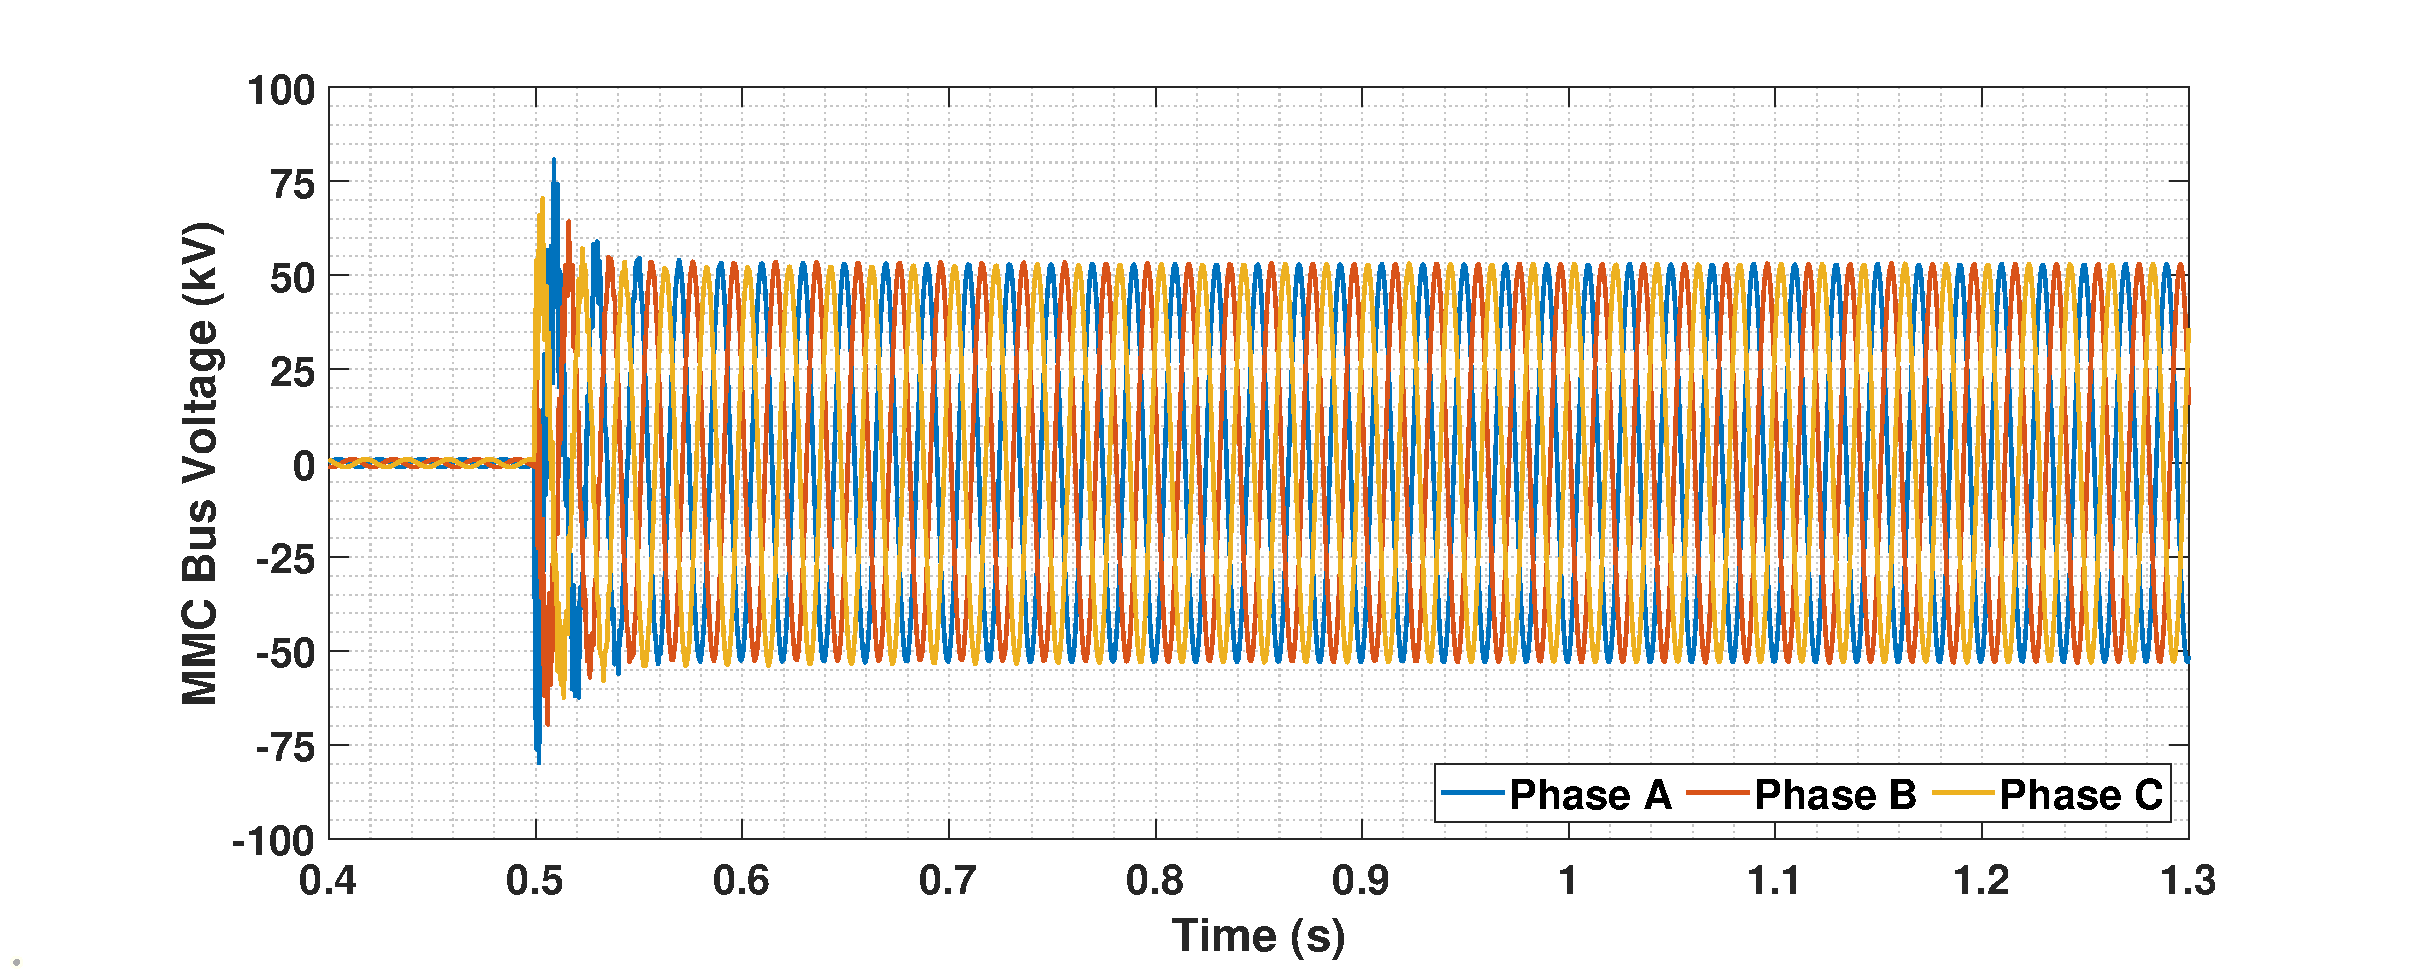
\includegraphics[height = 7.5cm,width = \textwidth]{Diagrams/Chapter_5/VABC_MMC_1_2_CB_5a.eps}
    \caption{Voltages at MMC bus upon CB-5a closing operation}
    \label{fig:VABC_MMC_1_2_CB_5a}
\end{figure}

\begin{figure}[H]
%\centering
%\hspace*{-1.2cm}
    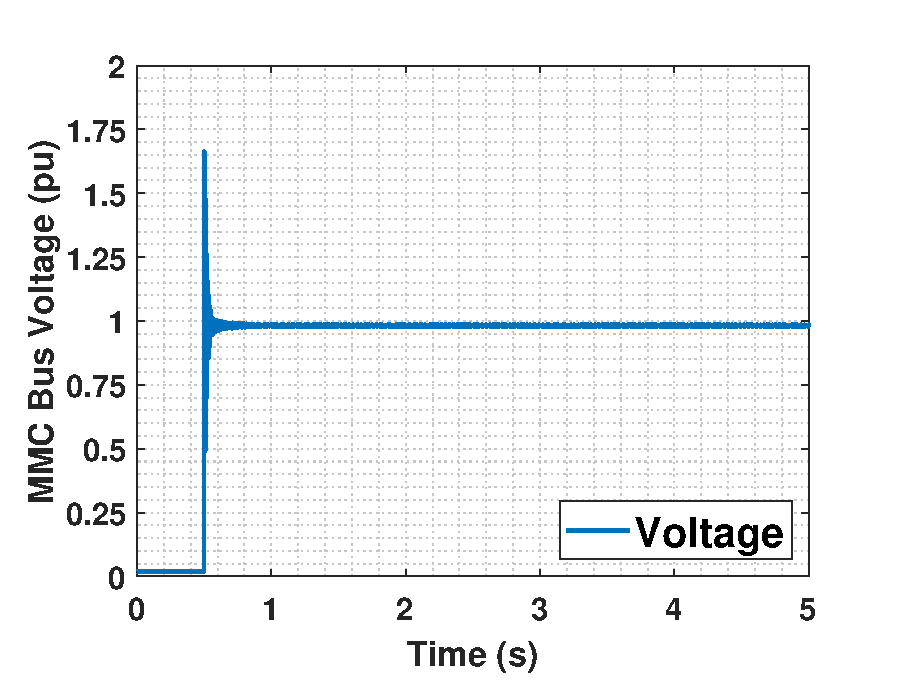
\includegraphics[height = 7cm,width = \textwidth]{Diagrams/Chapter_5/VACP_MMC_1_2_CB_5a.eps}
    \caption{Voltage in p.u. at MMC bus upon CB-5a closing operation}
    \label{fig:VACP_MMC_1_2_CB_5a}
\end{figure}

\begin{figure}[H]
%\centering
%\hspace*{-1.2cm}
\subfloat[Currents in MMC-1 bus]{%
  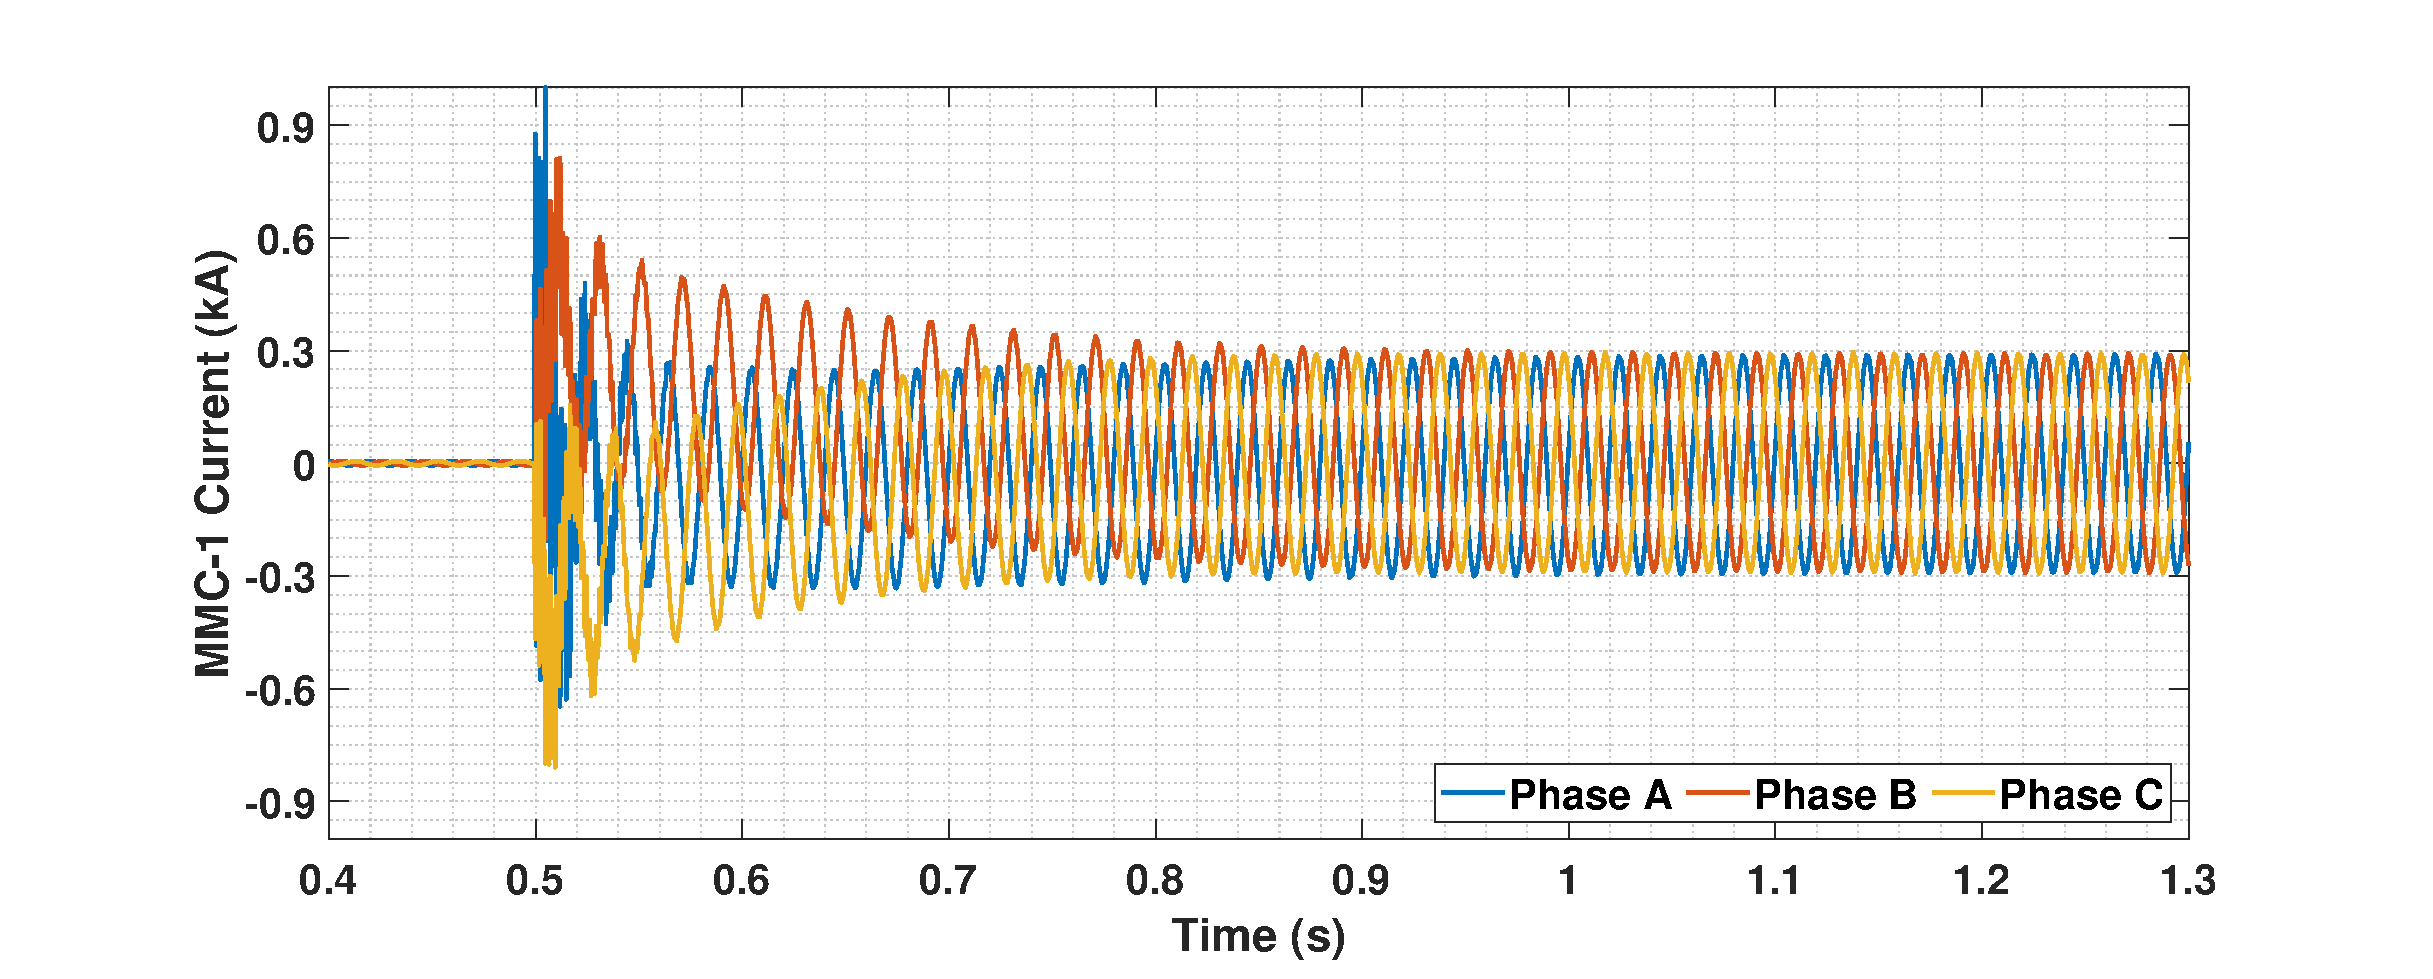
\includegraphics[height = 7cm,width = \textwidth]{Diagrams/Chapter_5/IABC_MMC_1_CB_5a.eps}%
\label{fig:IABC_MMC_1_CB_5a}}

%\hspace*{-1.2cm}
\subfloat[Currents in MMC-2 bus]{%
  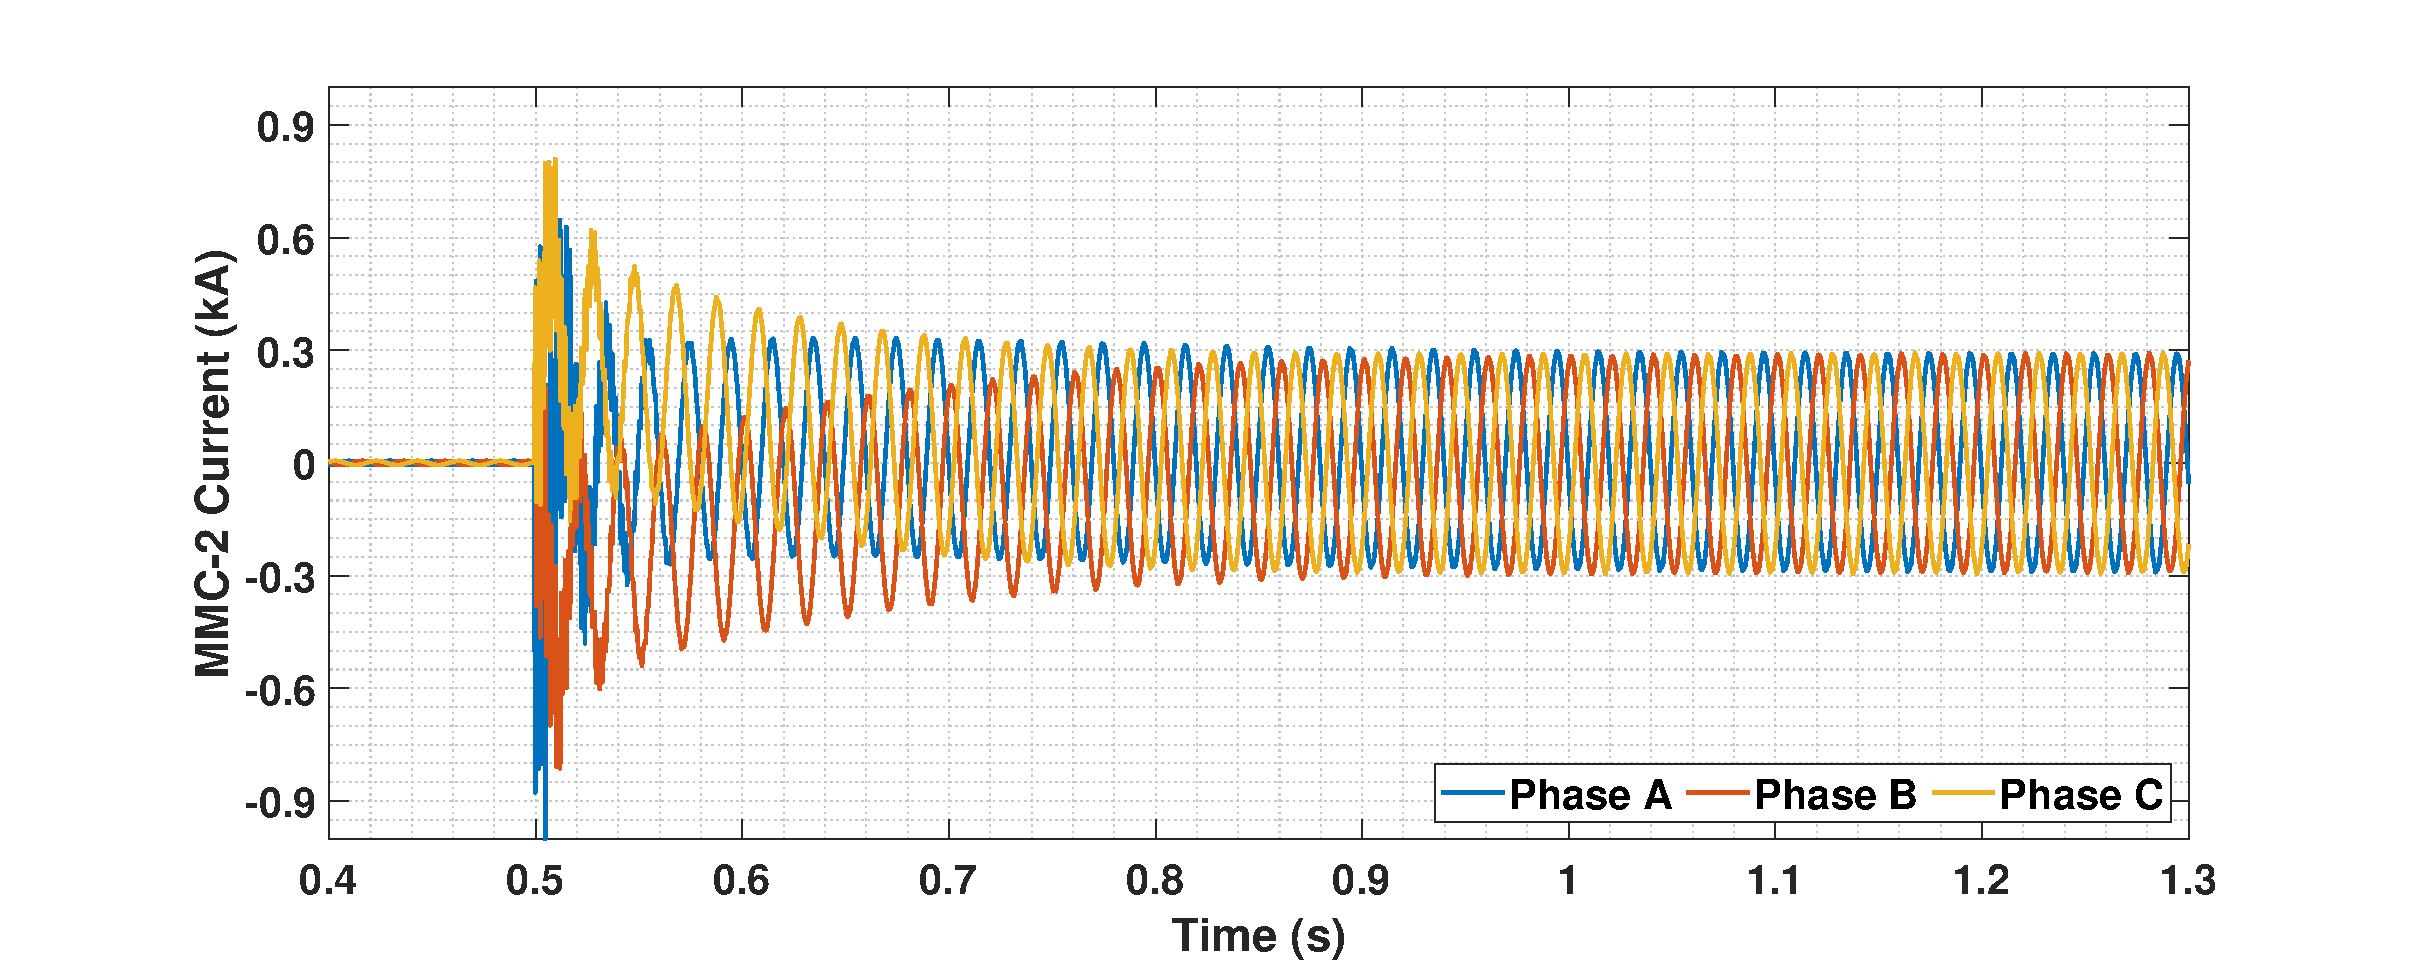
\includegraphics[height = 7cm,width = \textwidth]{Diagrams/Chapter_5/IABC_MMC_2_CB_5a.eps}%
\label{fig:IABC_MMC_2_CB_5a}}

\caption{Currents in a) MMC-1 bus and b) MMC-2 bus upon CB-5a closing operation}
\label{fig:IABC_MMC_1_2_CB_5a}
\end{figure}

The next step is to close the circuit breaker, CB-6a to connect \gls{MMC}-2 to the network and hence synchronizing it with \gls{MMC}-1. The voltage at the \gls{MMC} bus remains the same after connecting \gls{MMC}-2 as shown in Figure \ref{fig:VABC_MMC_1_2_CB_6a} and \ref{fig:VACP_MMC_1_2_CB_6a} since the voltage reference is provided and maintained by \gls{MMC}-1. The currents also remain the same in both the \gls{MMC}s after \gls{MMC}-2 connection as seen in Figure \ref{fig:IABC_MMC_1_CB_6a} and \ref{fig:IABC_MMC_2_CB_6a}. Now both the converter stations are synchronized and running.


\begin{figure}[H]
%\centering
%\hspace*{-1.2cm}
    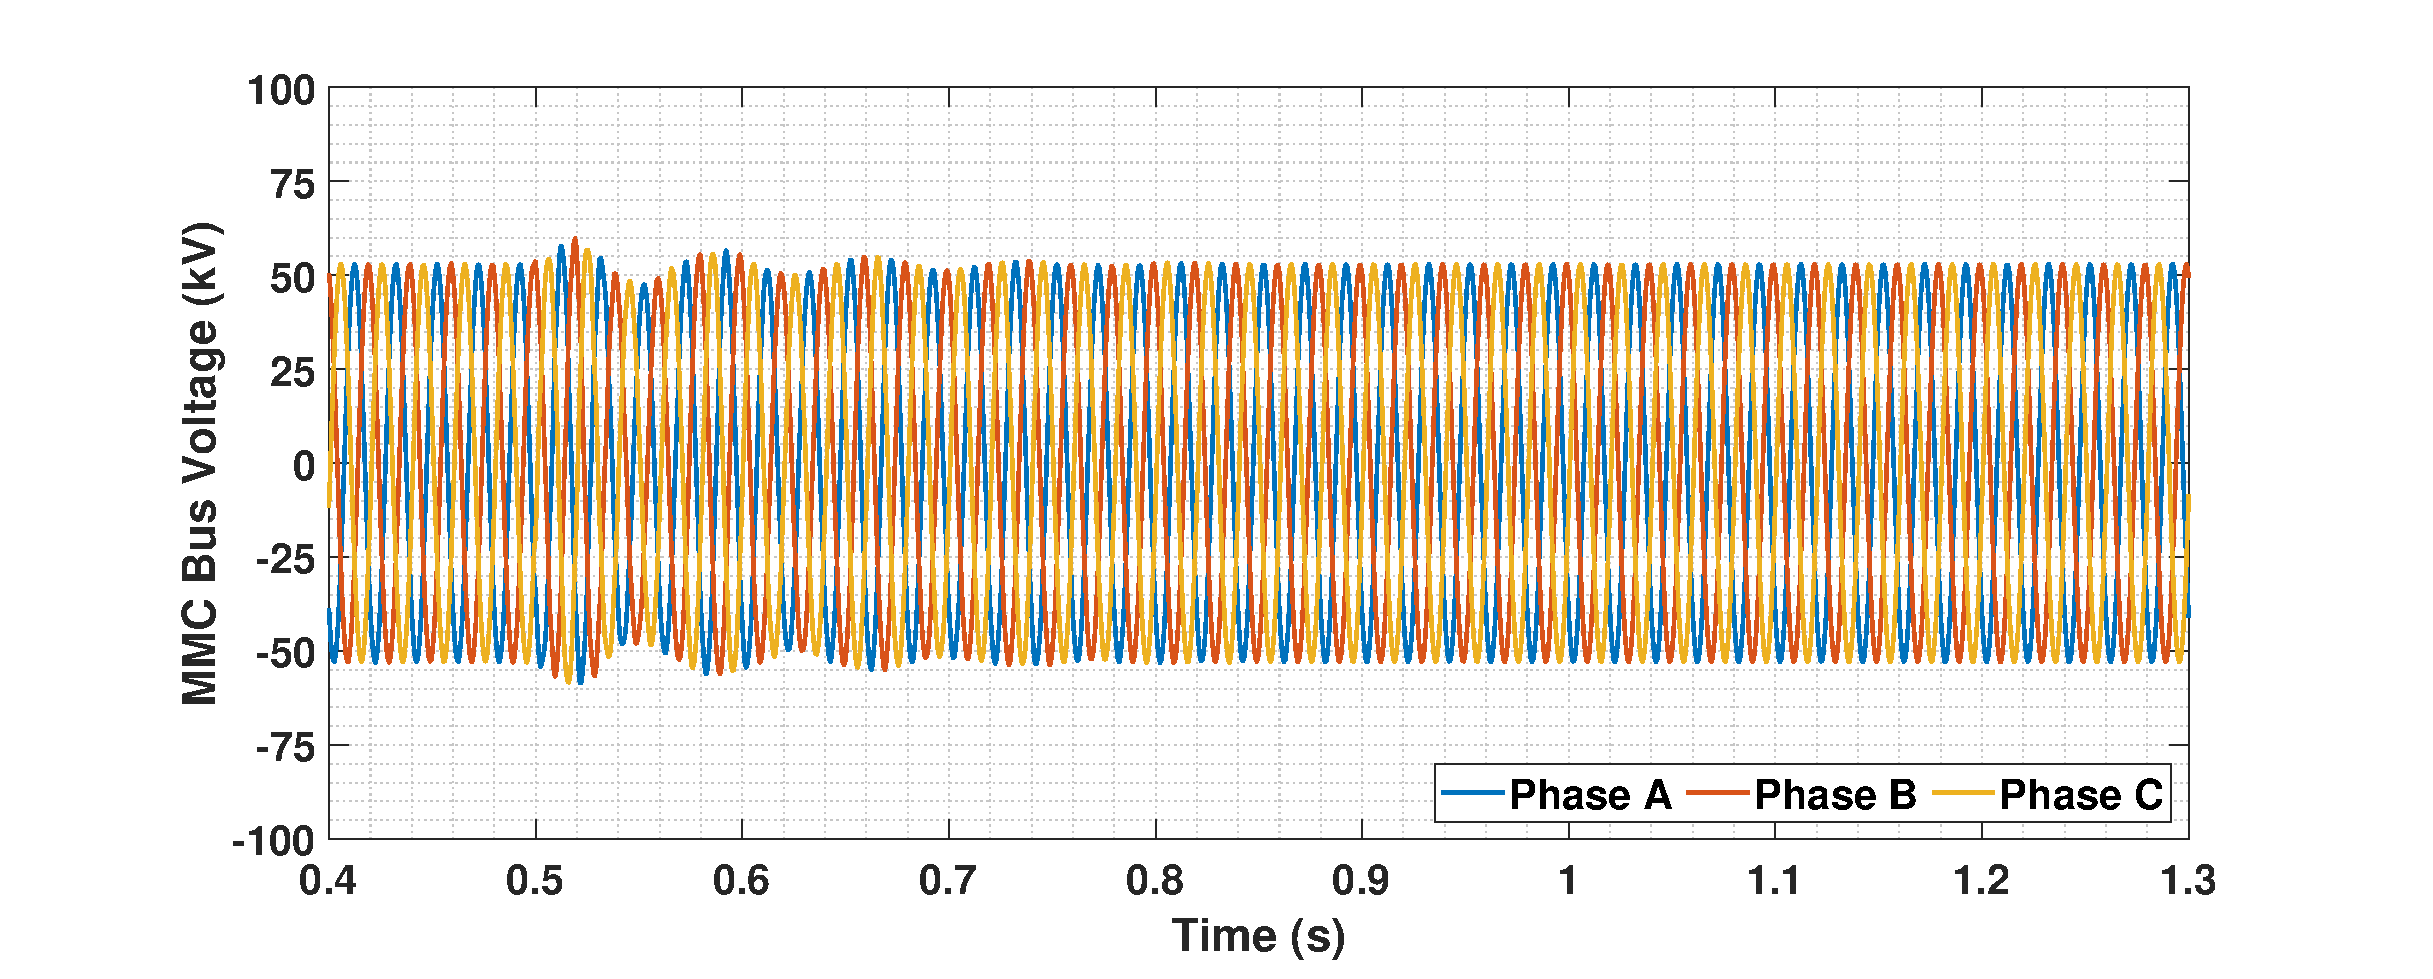
\includegraphics[height = 7.5cm,width = \textwidth]{Diagrams/Chapter_5/VABC_MMC_1_2_CB_6a.eps}
    \caption{Voltages at MMC bus upon CB-6a closing operation}
    \label{fig:VABC_MMC_1_2_CB_6a}
\end{figure}

\begin{figure}[H]
%\centering
%\hspace*{-1.2cm}
    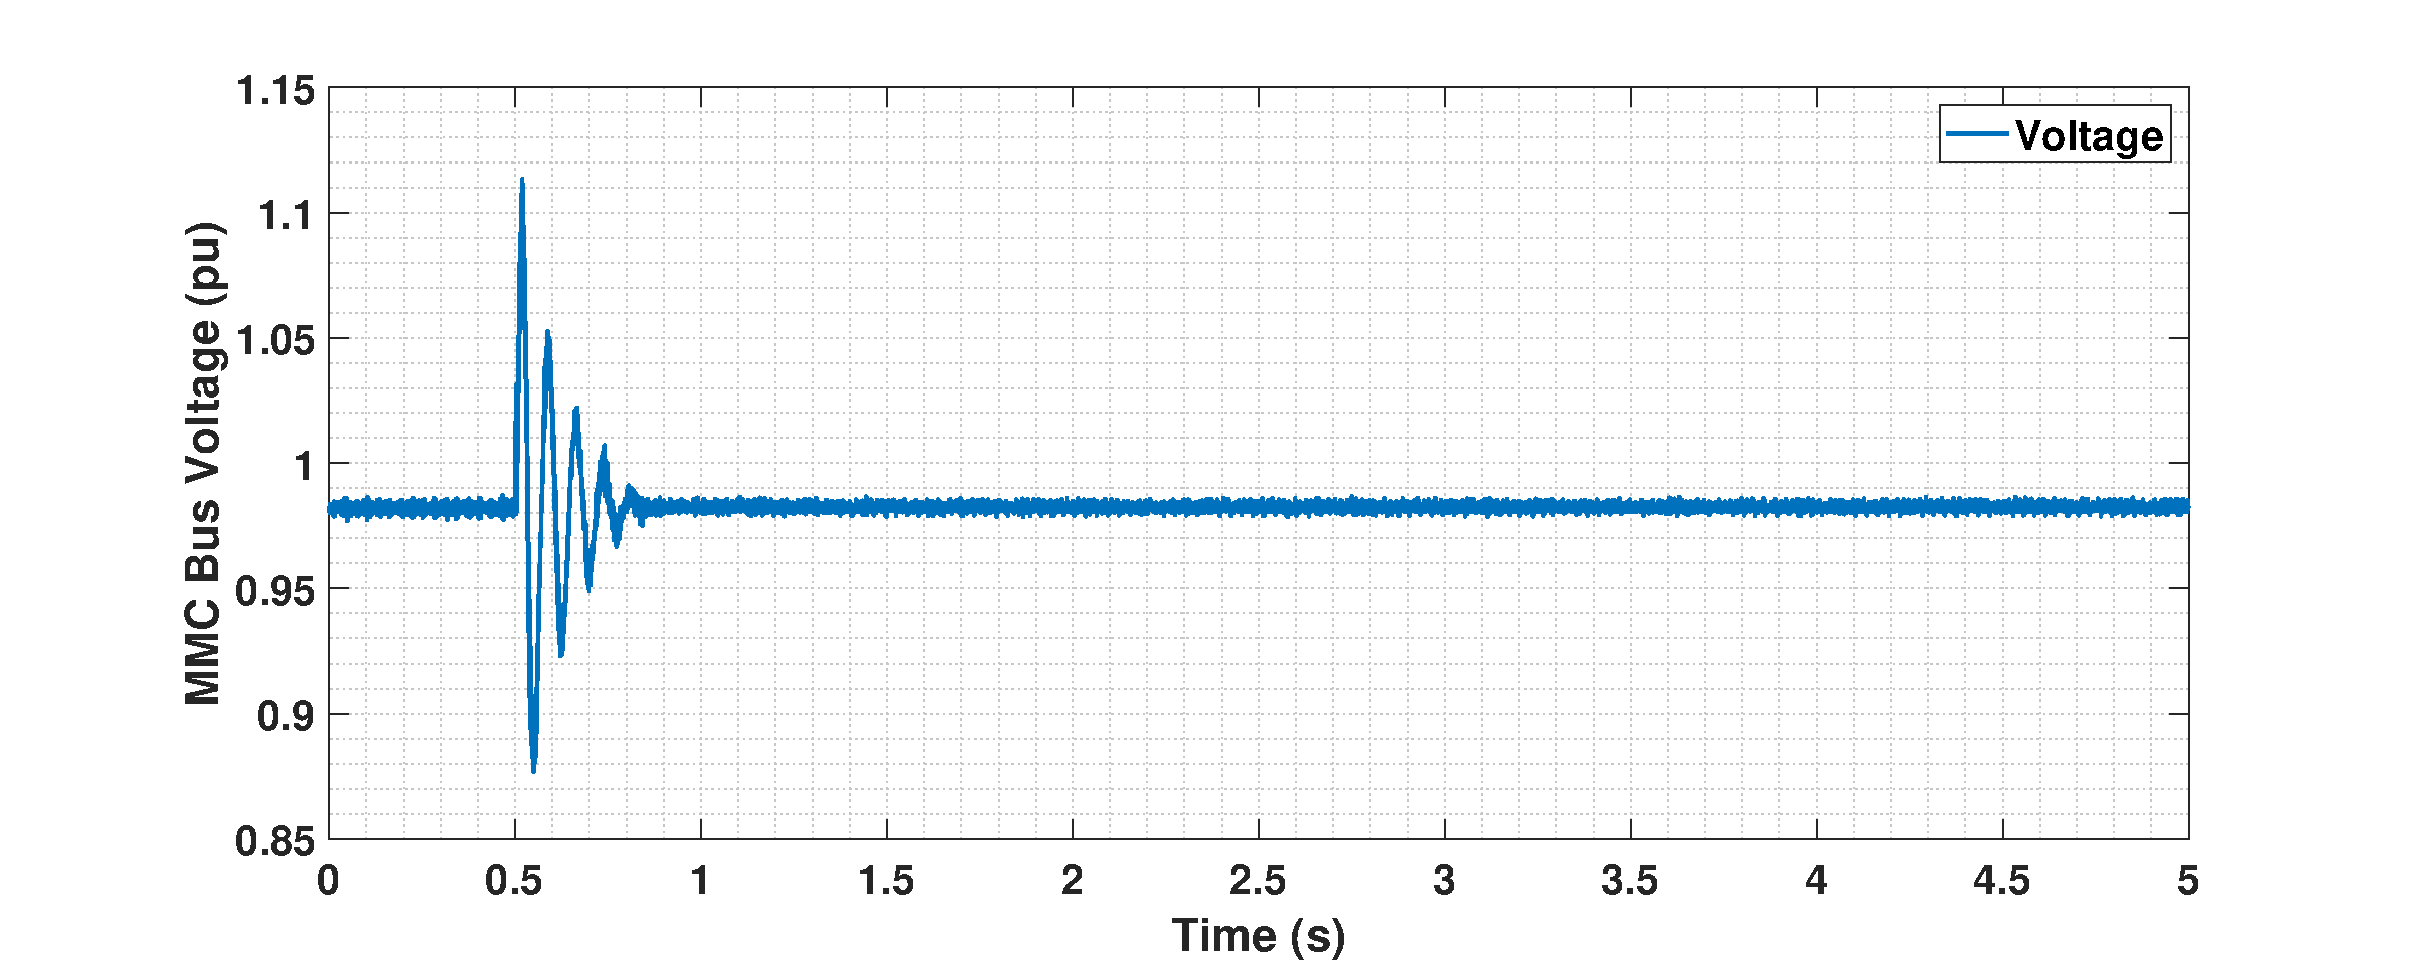
\includegraphics[height = 7.5cm,width = \textwidth]{Diagrams/Chapter_5/VACP_MMC_1_2_CB_6a.eps}
    \caption{Voltage in p.u. at MMC bus upon CB-6a closing operation}
    \label{fig:VACP_MMC_1_2_CB_6a}
\end{figure}

\begin{figure}[H]
%\centering
%\hspace*{-1.2cm}
\subfloat[Currents in MMC-1 bus]{%
  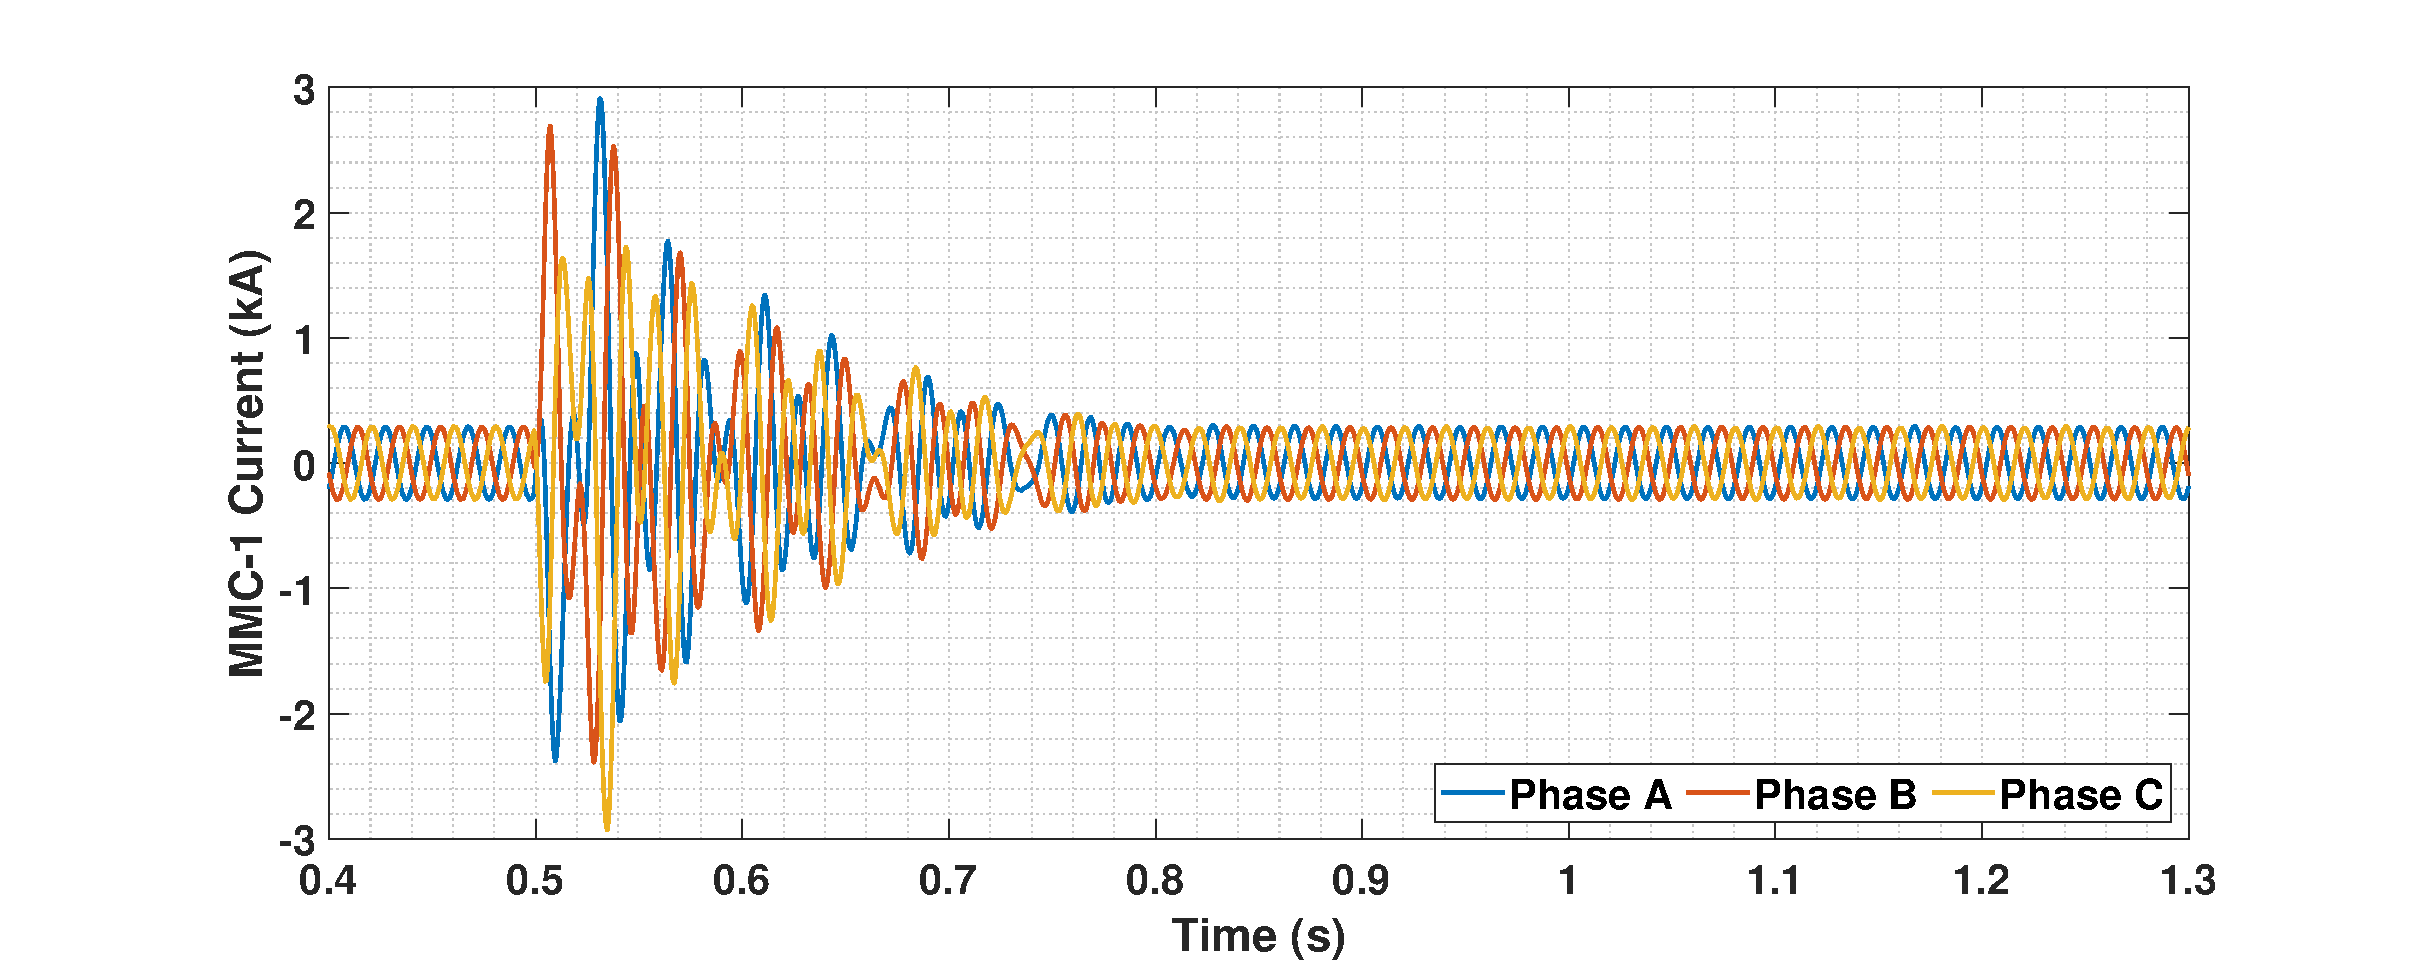
\includegraphics[height = 7.5cm,width = \textwidth]{Diagrams/Chapter_5/IABC_MMC_1_CB_6a.eps}%
\label{fig:IABC_MMC_1_CB_6a}}

%\hspace*{-1.2cm}
\subfloat[Currents in MMC-2 bus]{%
  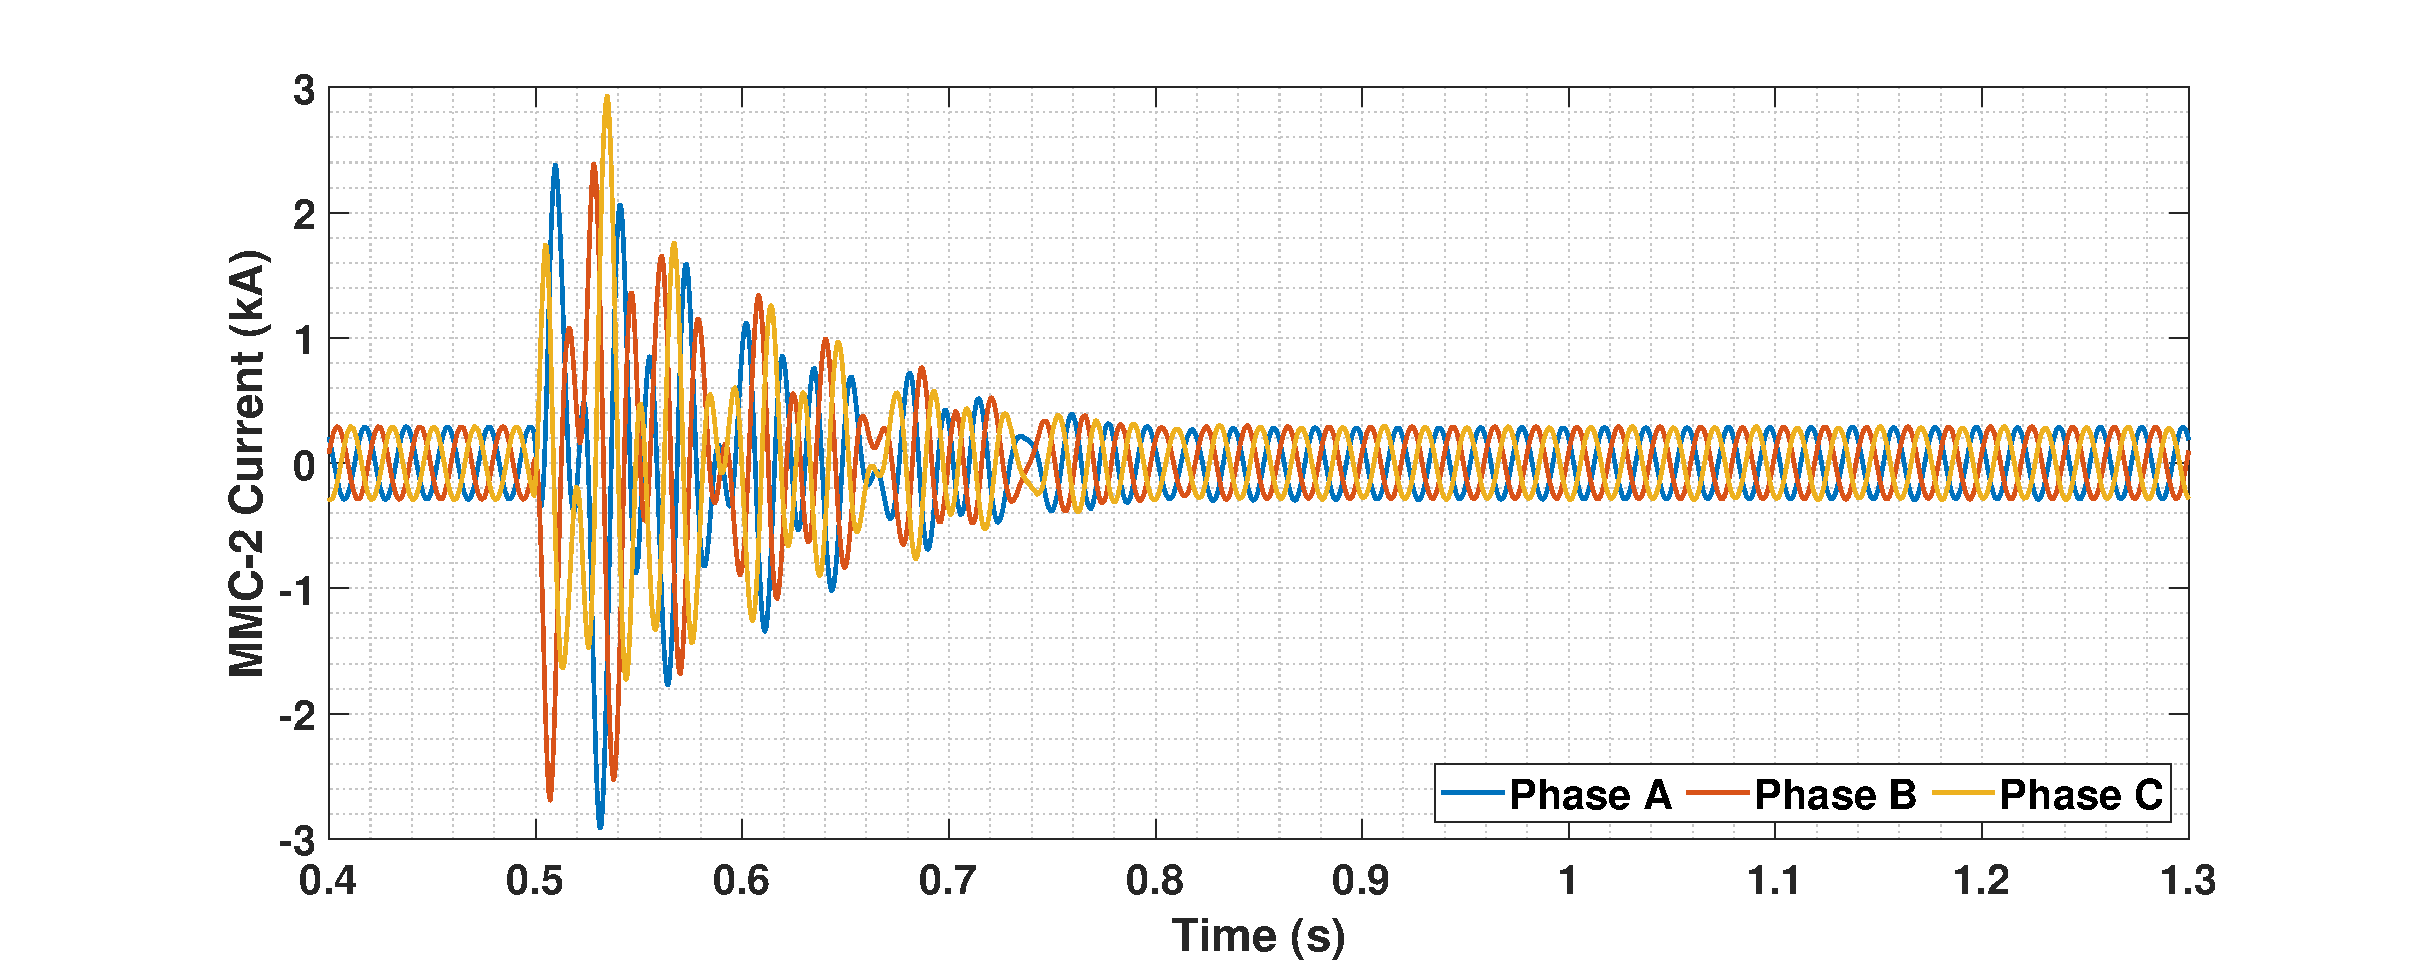
\includegraphics[height = 7.5cm,width = \textwidth]{Diagrams/Chapter_5/IABC_MMC_2_CB_6a.eps}%
\label{fig:IABC_MMC_2_CB_6a}}

\caption{Currents in a) MMC-1 bus and b) MMC-2 bus upon CB-6a closing operation}
\label{fig:IABC_MMC_1_2_CB_6a}
\end{figure}

\section{Energization of the HVAC Cables and OWFs}\label{energization_HVAC_Cables}
The energization procedure of the \gls{AC} network followed in this work involves charging of each \gls{HVAC} cable and the corresponding \gls{OWF}. Initially, cable-1 is charged and then \gls{OWF}-1 is connected. The same is followed for the other \gls{OWF}s as well. As mentioned in Section \ref{Aggregated_OWF_large_scale} in Chapter \ref{4}, each \gls{OWF} has a maximum capacity of 500 MW that is represented by scaling up (by using the scaling factor function in RSCAD) of a \gls{WG} model of 6 MW rated power. For the energization process, the \gls{OWF}s are connected initially with lesser number of \gls{WG} units of $\sim{50}$ MW (8 $\times$ 6 MW = 48 MW) power to avoid a surge of voltage at \gls{PCC} and to maintain the voltage within limits. Once stability is attained after connecting all the \gls{OWF}s, the scaling in all \gls{OWF}s is incremented. Since power only flows through \gls{MMC}-1 until then, the increment can be until the maximum capacity of \gls{MMC}-1, i.e. 1 GW.

The cable-1 gets energized when the CB-1a circuit breaker, as shown in Figure \ref{fig:WT4_MMC2_Chap5}, is switched on. The voltage at \gls{MMC} bus is increased and set to a value of nearly 1.05 p.u. as seen in Figure \ref{VACP_MMC_bus_Cab1charg}. \gls{MMC}-1 provides the current for cable charging and the active power reference for the \gls{MMC}-2 is not changed in this process. Hence, current flow in \gls{MMC}-1 bus increases for cable-1 charging as shown in Figure \ref{fig:IABC_MMC_1_Cab1charg} and the current flow in \gls{MMC}-2 bus remains unchanged as shown in Figure \ref{fig:IABC_MMC_2_Cab1charg}. The disturbances observed during the switching operation at 0.5 seconds, before the currents stabilize to a particular value at 0.75 seconds, is due to the \gls{PI} parameters chosen for the V/F control in \gls{MMC}-1. Optimizing these parameters through small-signal stability analysis could achieve smoother results. The current in cable-1 upon CB-1a closing is depicted in Figure \ref{fig:IABC_Cab1_Cab1charg}. 

\begin{figure}[H]
%\centering
%\hspace*{-1.2cm}
    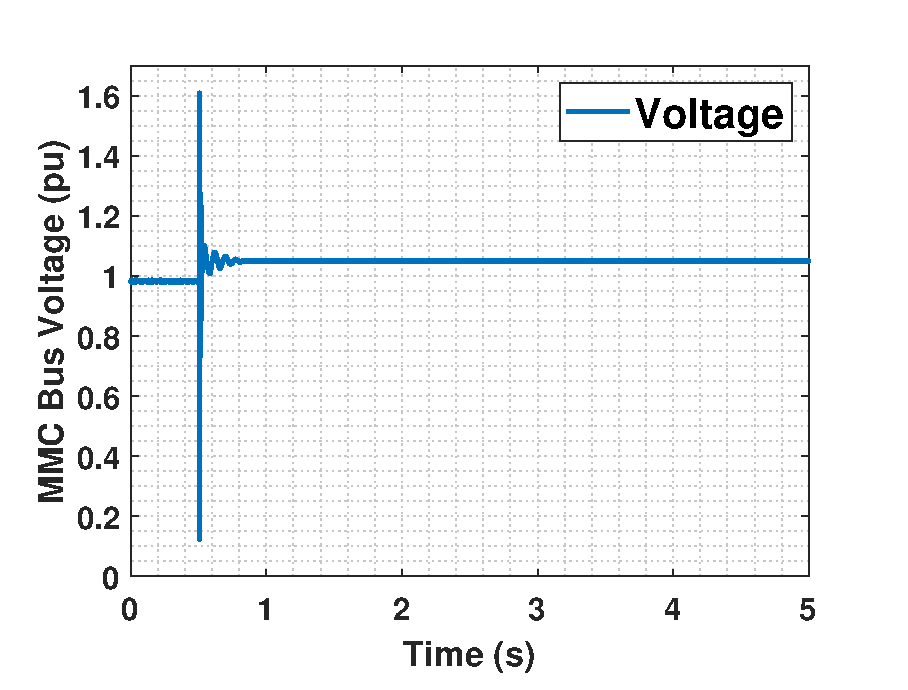
\includegraphics[height = 7cm,width = \textwidth]{Diagrams/Chapter_5/VACP_MMC_bus_Cab1charg.eps}
    \caption{Voltage at MMC bus upon charging of cable-1}
    \label{VACP_MMC_bus_Cab1charg}
\end{figure}

\begin{figure}[H]
%\centering
%\hspace*{-1.2cm}
\subfloat[Currents in MMC-1 bus]{%
  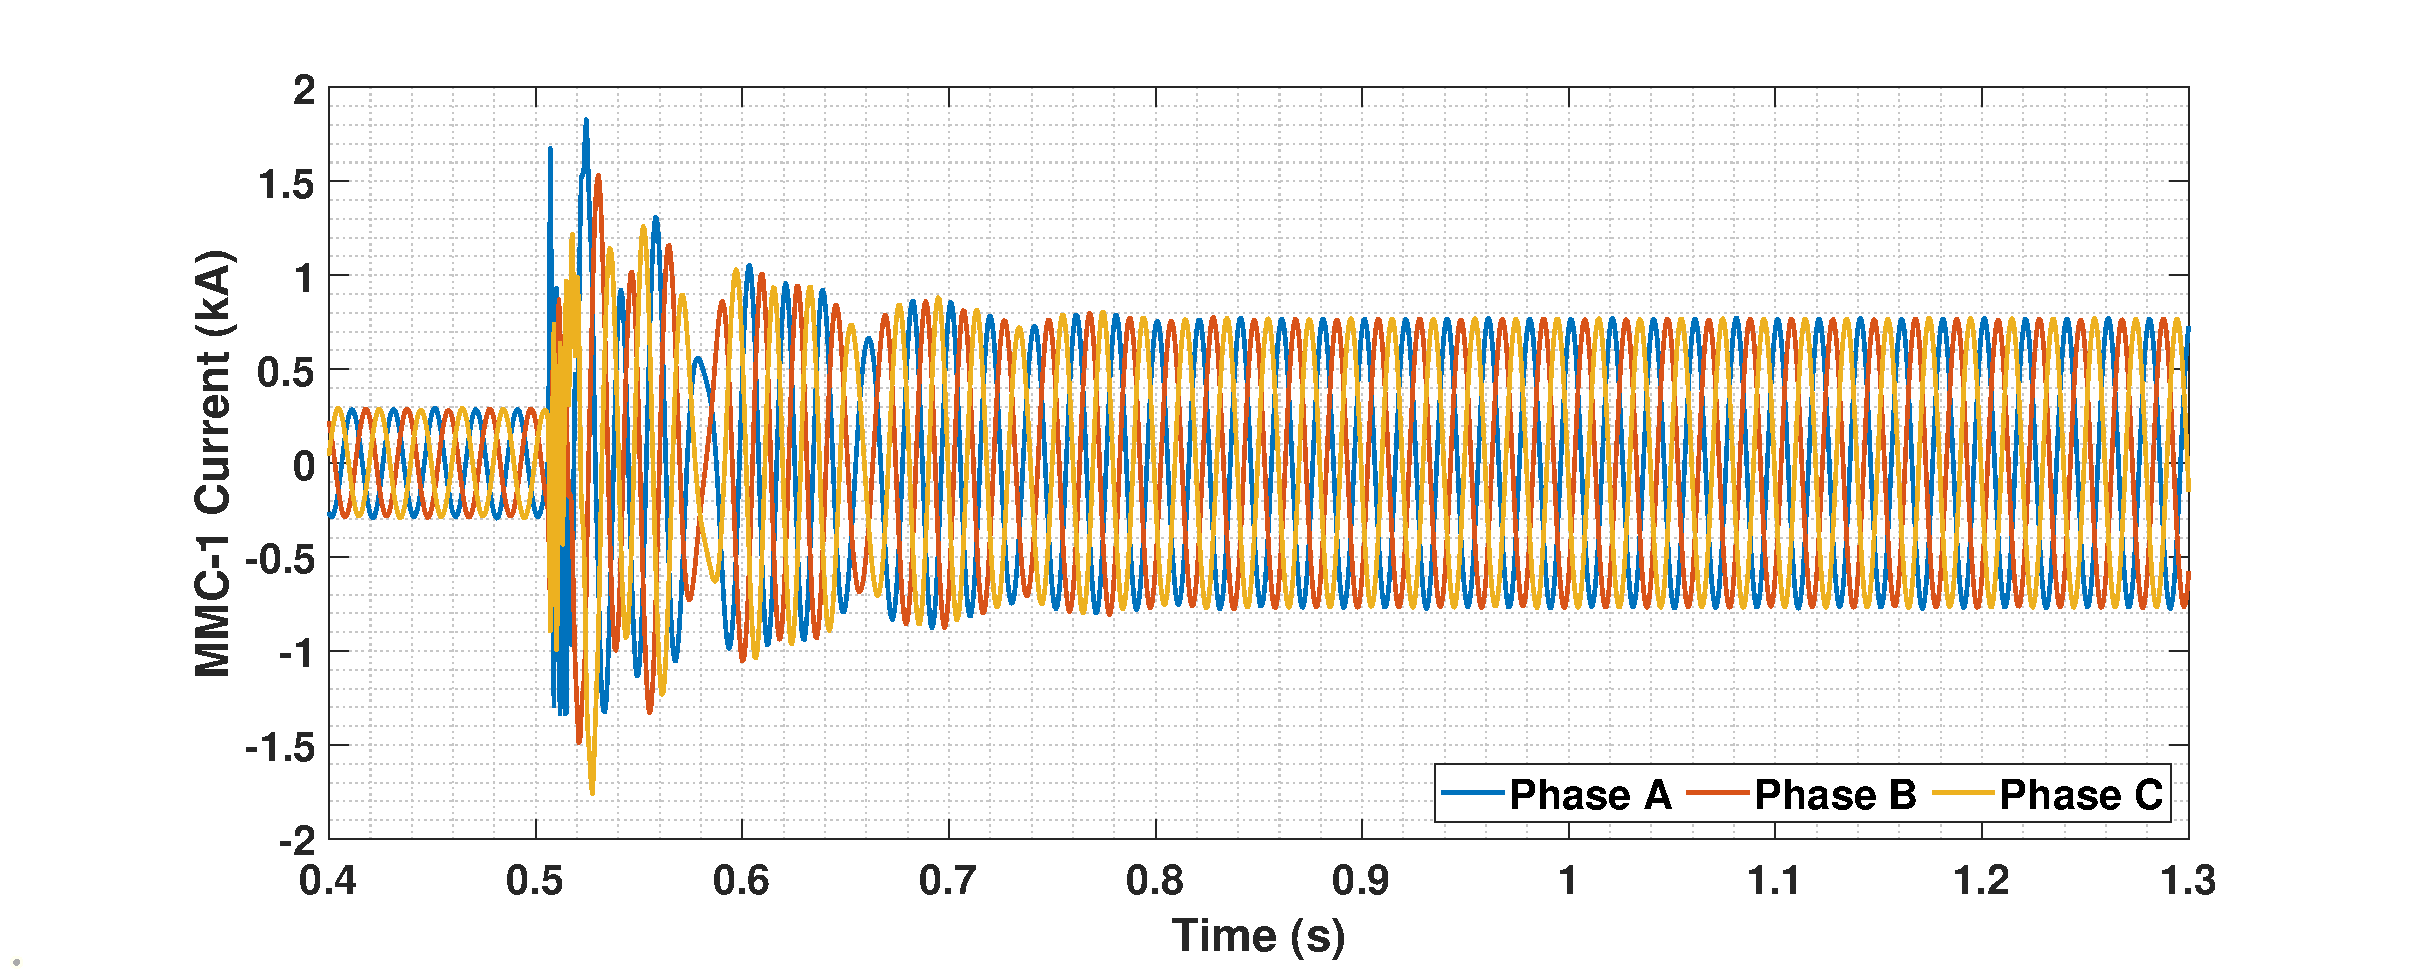
\includegraphics[height = 7cm,width = \textwidth]{Diagrams/Chapter_5/IABC_MMC_1_Cab1charg.eps}%
\label{fig:IABC_MMC_1_Cab1charg}}

%\hspace*{-1.2cm}
\subfloat[Currents in MMC-2 bus]{%
  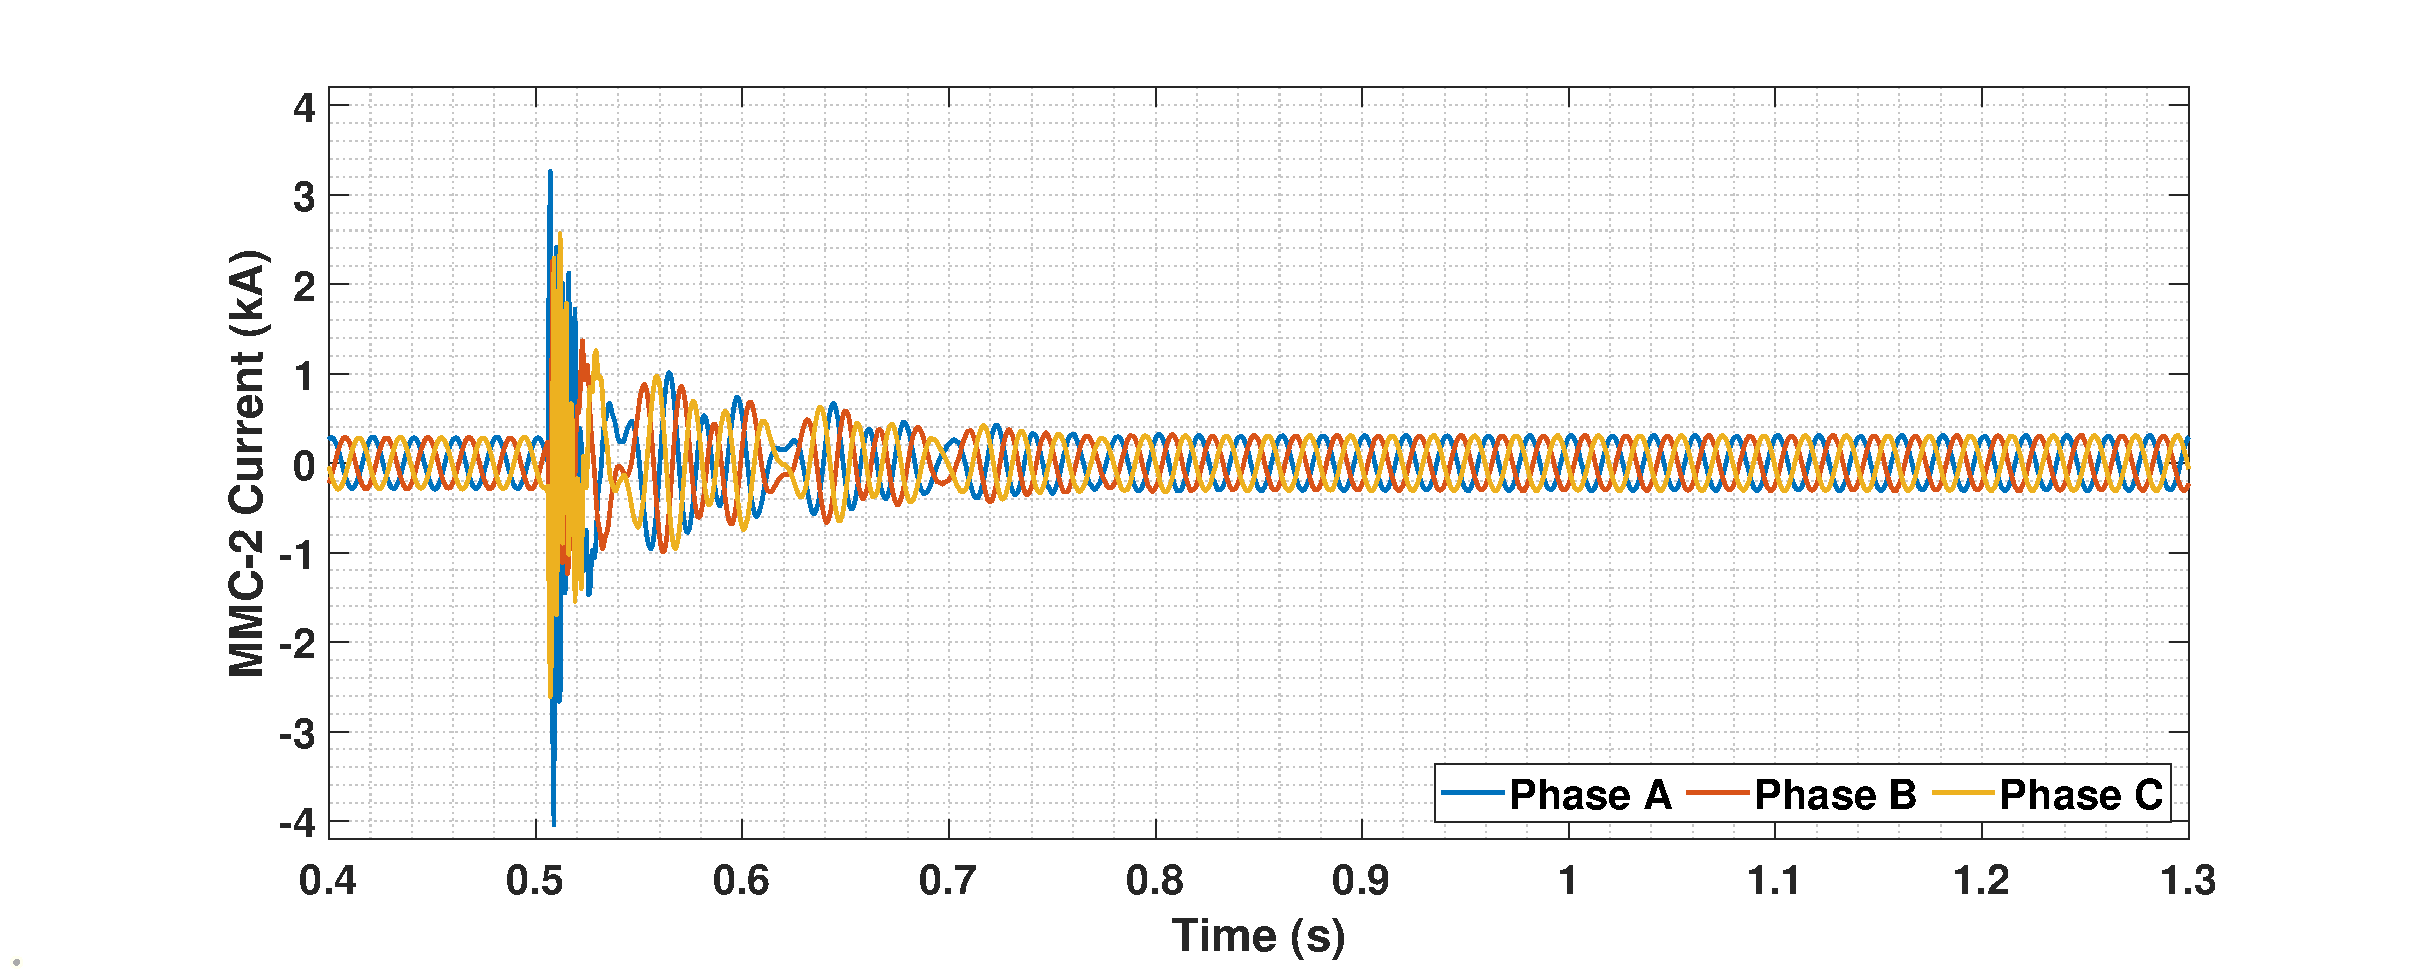
\includegraphics[height = 7cm,width = \textwidth]{Diagrams/Chapter_5/IABC_MMC_2_Cab1charg.eps}%
\label{fig:IABC_MMC_2_Cab1charg}}

\caption{Currents in a) MMC-1 bus b) MMC-2 bus upon CB-1a closing operation for charging of cable-1}
\label{fig:IABC_MMC_1_2_CB_Cab1charg}
\end{figure}

\begin{figure}[H]
%\centering
%\hspace*{-1.2cm}
    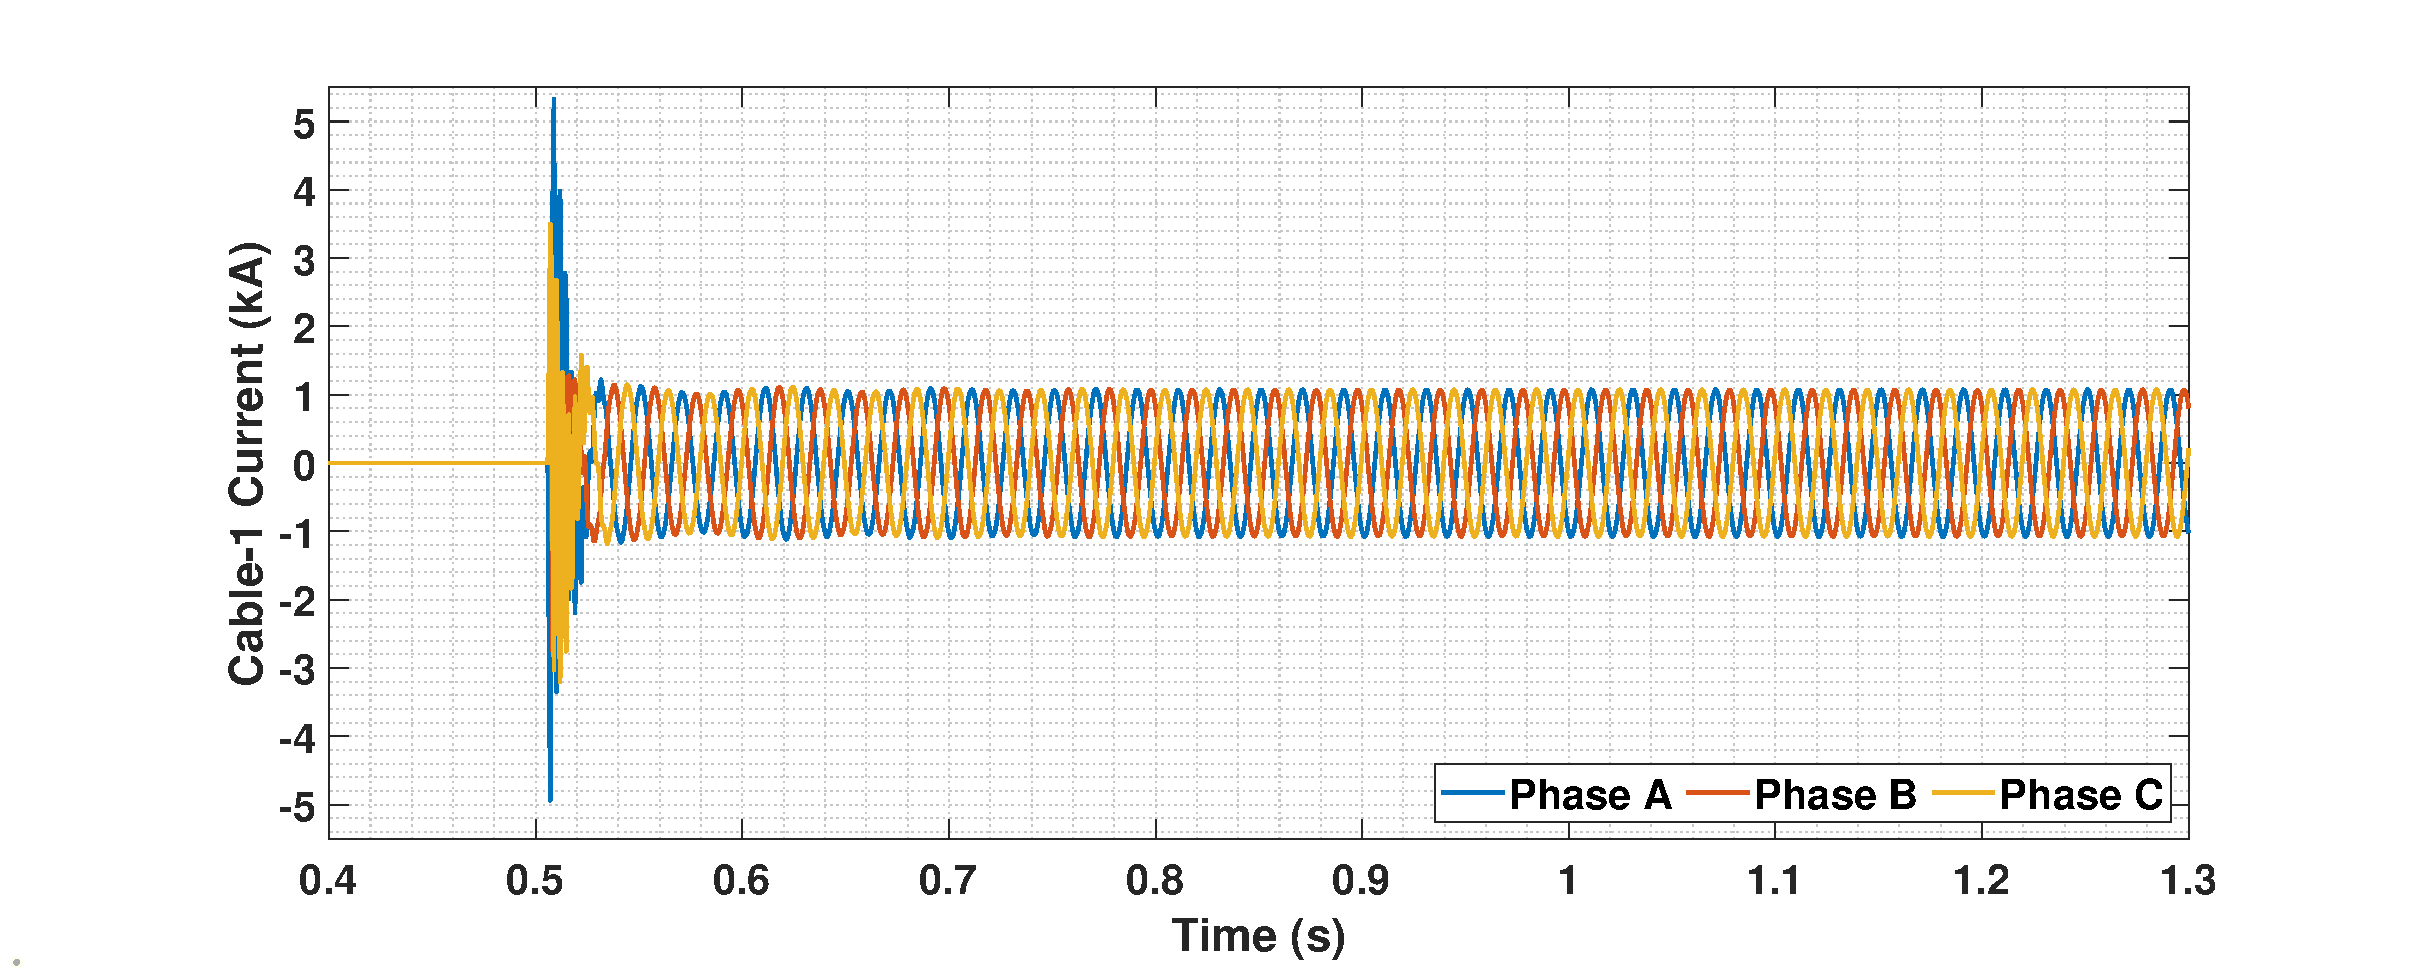
\includegraphics[height = 7cm,width = \textwidth]{Diagrams/Chapter_5/IABC_Cab1_Cab1charg.eps}
    \caption{Currents in cable-1 upon CB-1a closing operation for charging of cable-1}
    \label{fig:IABC_Cab1_Cab1charg}
\end{figure}

After cable-1 has been charged, the breaker at the \gls{OWF}-1 end (CB-1b) is switched on. \gls{OWF}-1 gets connected to the network. As mentioned in Section \ref{energization_HVAC_Cables}, the \gls{OWF}-1 is connected initially with less generation to keep the voltage at \gls{PCC}-1 within limits. The initial high voltage at the \gls{PCC}-1 before closing the breaker as seen in Figure \ref{VACP_WT1_WT1connect} is due to the capacitance in the DC link. Once the breaker is closed, the voltage is maintained at nearly 1 p.u. as shown in Figure \ref{VACP_WT1_WT1connect} and the currents in \gls{PCC}-1 also increase as shown in Figure \ref{IABC_WT1_WT1connect}. The \gls{OWF} starts generating 50 MW and this flows through \gls{MMC}-1 as shown in Figure \ref{P_MMC_1_WT1234connect}. In a similar way all the other \gls{OWF}s are connected. All \gls{OWF}s are connected with $\sim{50}$ MW generation. A total power of $\sim{200}$ MW through \gls{MMC}-1 after connection of \gls{OWF}-1, \gls{OWF}-2, \gls{OWF}-3 and \gls{OWF}-4 is clearly depicted in Figure \ref{P_MMC_1_WT1234connect}. There is no flow of active power in \gls{MMC}-2 (Figure \ref{P_MMC_2_WT1234connect}) since the rated capacity of 1 GW of \gls{MMC}-1 is yet to be reached. %The delay before connecting \gls{OWF}-4 at 0.5 s, that is depicted in the purple line in Figure \ref{P_MMC_1_WT1234connect} and Figure \ref{P_MMC_2_WT1234connect}, is due to the time delay in measurement of the signals.

\begin{figure}[H]
%\centering
%\hspace*{-1.2cm}
    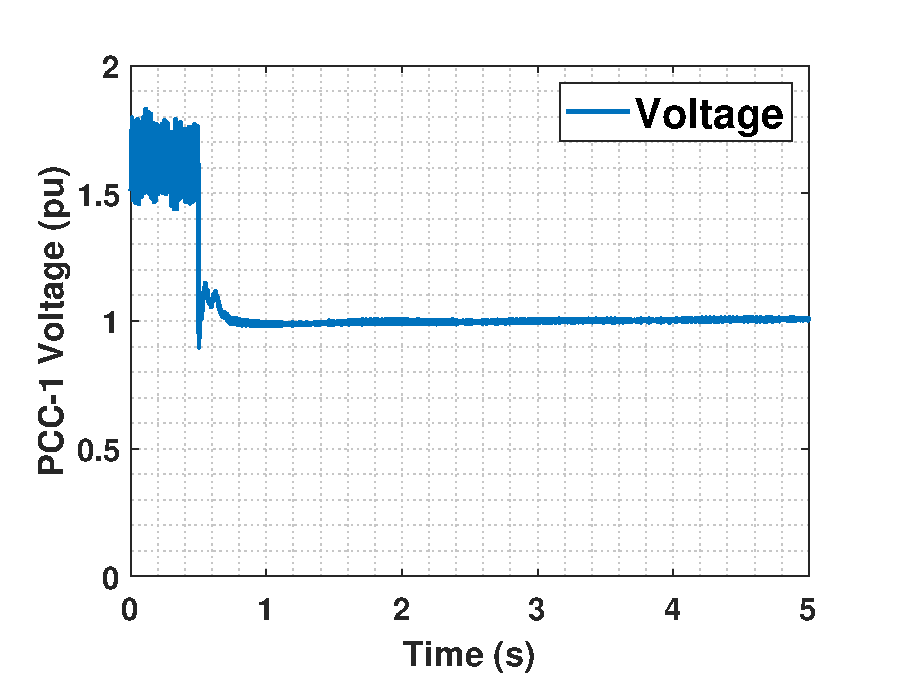
\includegraphics[height = 7cm,width = \textwidth]{Diagrams/Chapter_5/VACP_WT1_WT1connect.eps}
    \caption{Voltage in p.u. at PCC-1 upon connecting OWF-1 with 50 MW generation to the network}
    \label{VACP_WT1_WT1connect}
\end{figure}

\begin{figure}[H]
%\centering
%\hspace*{-1.2cm}
    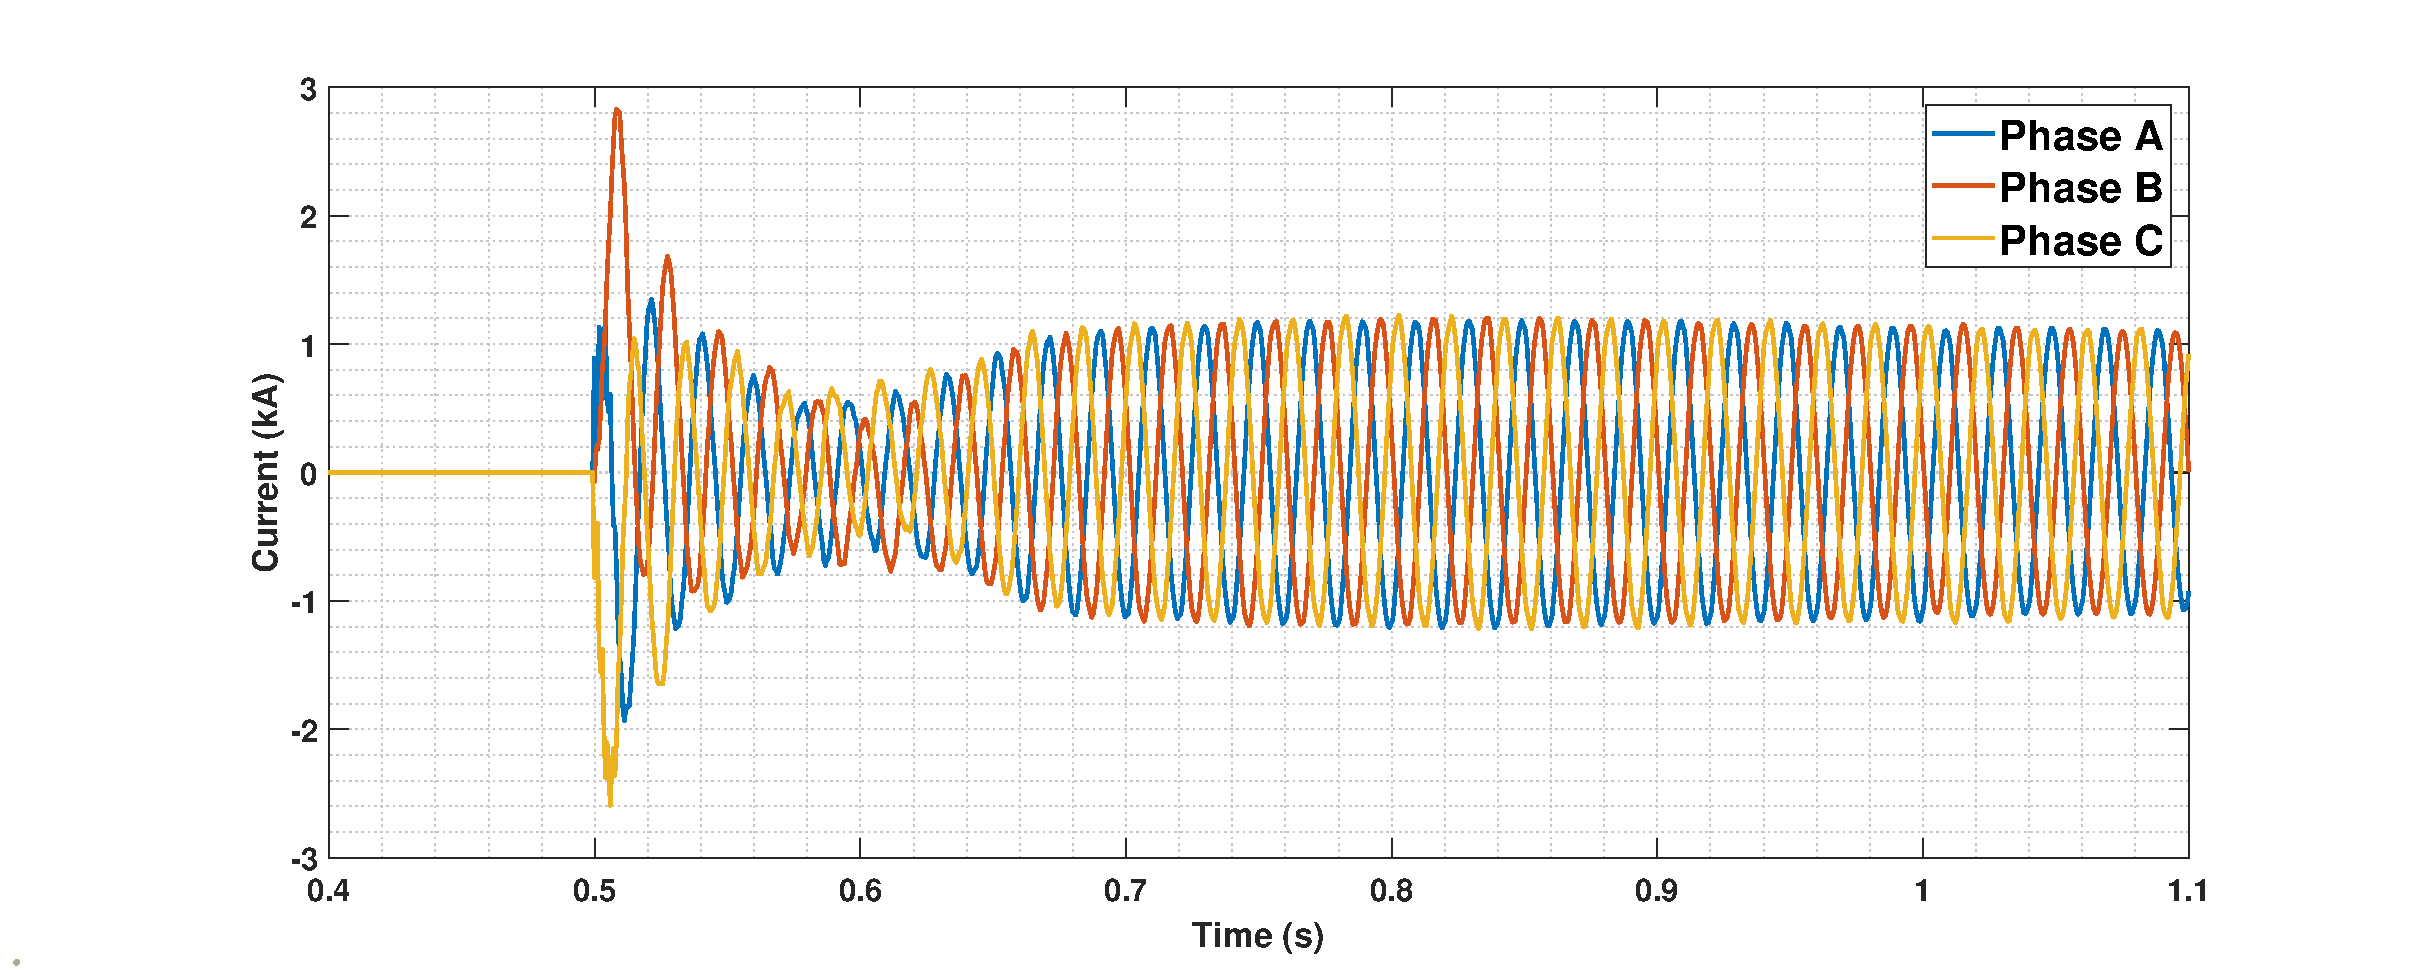
\includegraphics[height = 7cm,width = \textwidth]{Diagrams/Chapter_5/IABC_WT1_WT1connect.eps}
    \caption{Currents in PCC-1 upon connecting OWF-1 with 50 MW generation to the network}
    \label{IABC_WT1_WT1connect}
\end{figure}

\begin{figure}[H]
%\centering
%\hspace*{-1.2cm}
    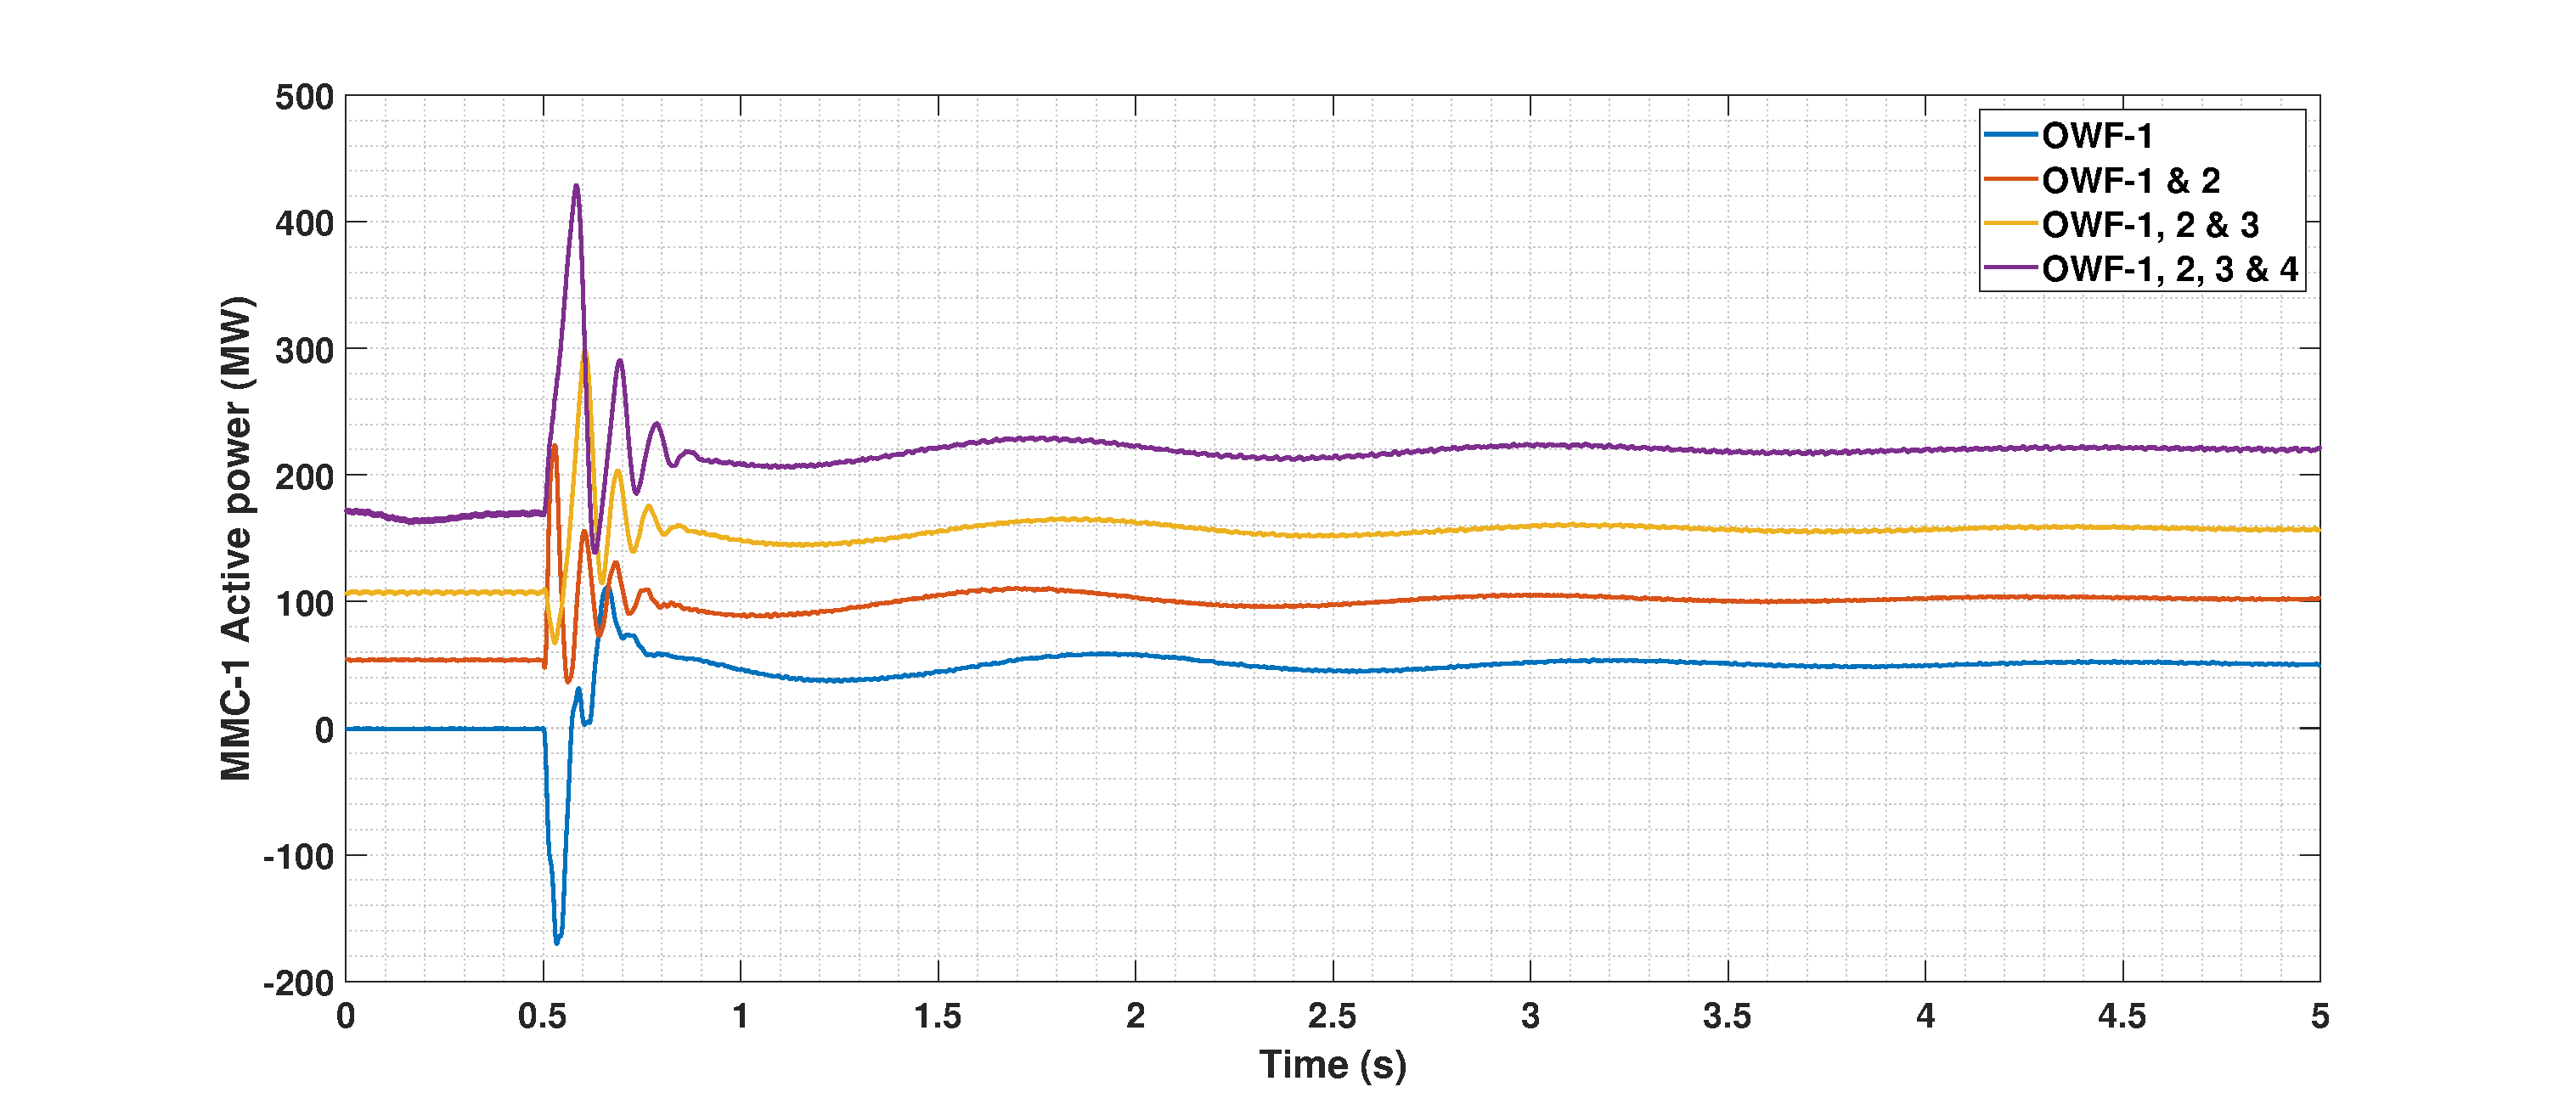
\includegraphics[height = 7cm,width = \textwidth]{Diagrams/Chapter_5/P_MMC_1_WT1234connect_2.eps}
    \caption{Active power in MMC-1 bus upon connecting all OWFs with 50 MW generation each}
    \label{P_MMC_1_WT1234connect}
\end{figure}

\begin{figure}[H]
%\centering
%\hspace*{-1.2cm}
    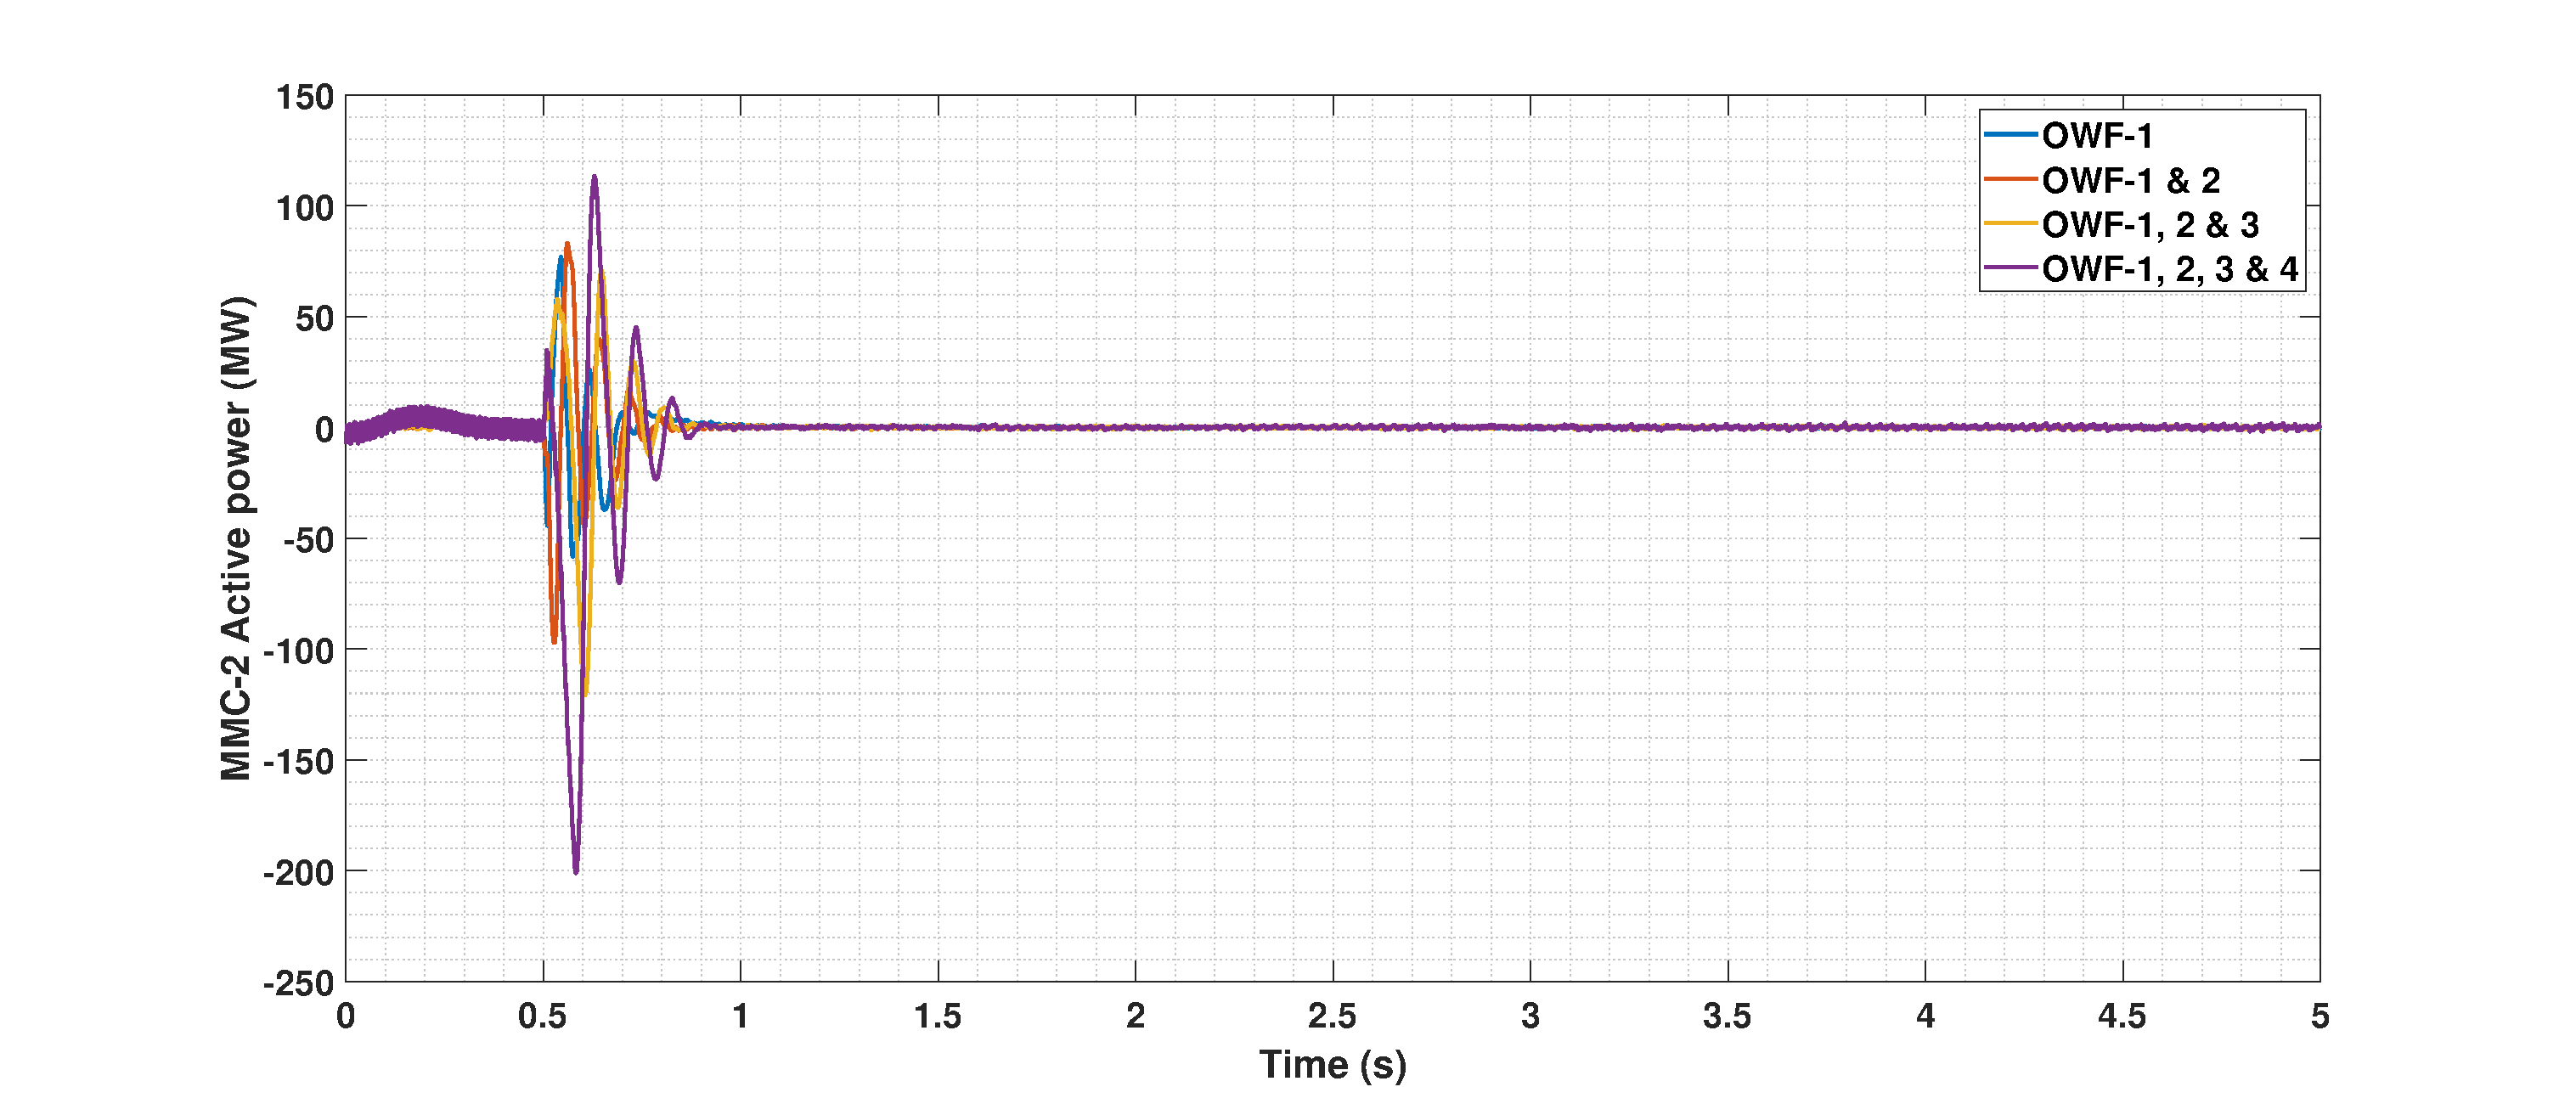
\includegraphics[height = 7cm,width = \textwidth]{Diagrams/Chapter_5/P_MMC_2_WT1234connect_2.eps}
    \caption{Active power in MMC-2 bus upon connecting all OWFs with 50 MW generation each}
    \label{P_MMC_2_WT1234connect}
\end{figure}

Once the system gets stabilized, the generation is increased in steps by increasing the number of parallel \gls{WG} units. Such a procedure ensures the voltage to be within limits at all \gls{PCC}s. The power flow to the \gls{MMC}-2 is to be controlled in the next step. This is done by controlling the active power reference of \gls{MMC}-2. For this study, \gls{OWF}s are modelled to have the same scaling of power and hence generate the same amount of power. A step-by-step increment of $\sim{50}$ MW in all \gls{OWF} is done, and correspondingly the active power reference for \gls{MMC}-2 is also increased. The procedure is detailed in Appendix \ref{steps_energ_appen}. Finally, the \gls{OWF}s are made to generate $\sim{500}$ MW each and the total of nearly 2 GW power is equally split between \gls{MMC}-1 and \gls{MMC}-2. Power losses are expected to occur during the transmission and, hence the active power flowing is nearly 960 MW in both \gls{MMC}s as seen from the final steady state plots in Figure \ref{P_MMC_1_2_All_WTconnect}.

\begin{figure}[H]
\centering
%\hspace*{-1cm}
    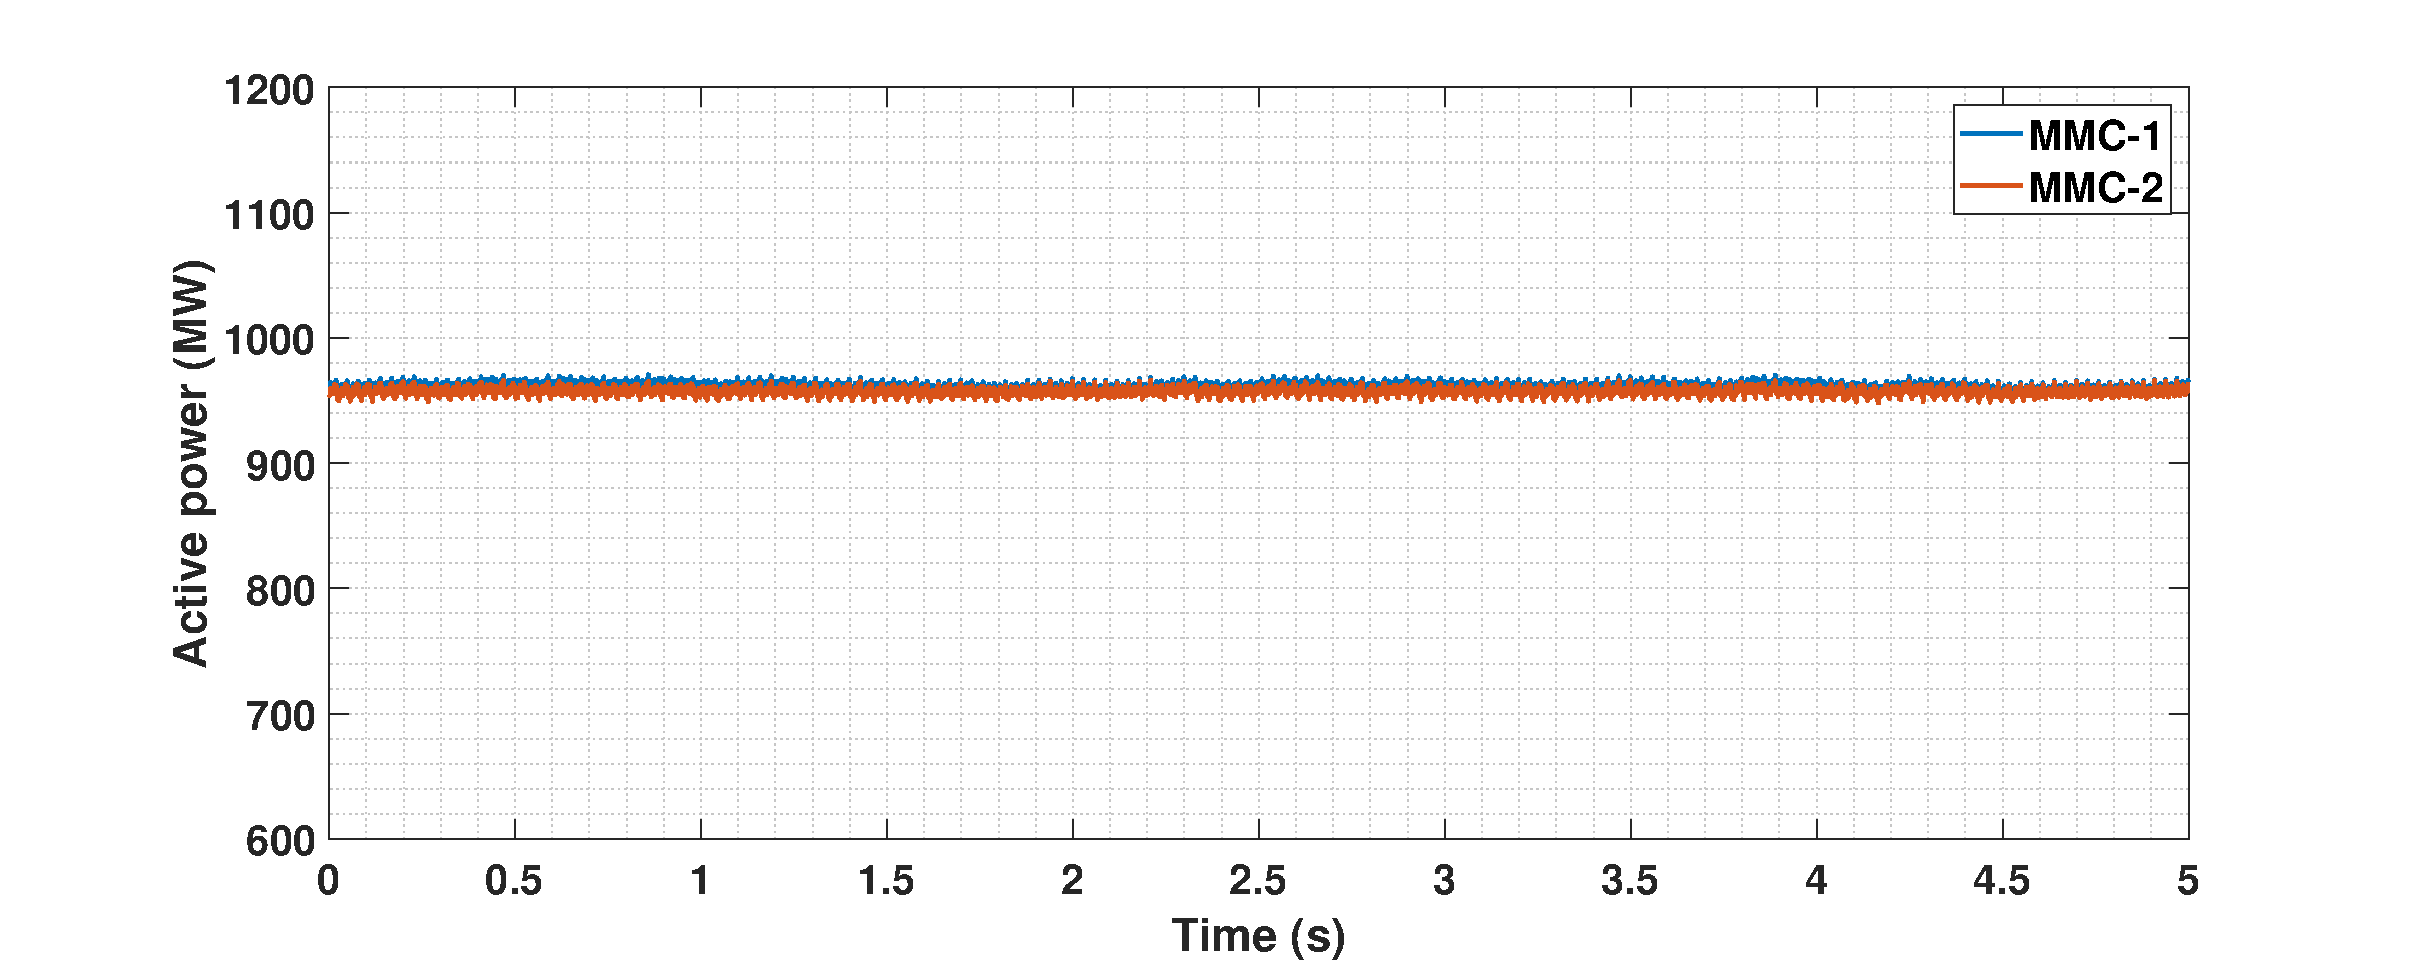
\includegraphics[height = 7cm,width = \textwidth]{Diagrams/Chapter_5/P_MMC_1_2_All_WTconnect.eps}
    \caption{Active power in MMC-1 and MMC-2 buses upon connecting all OWFs with 500 MW generation each}
    \label{P_MMC_1_2_All_WTconnect}
\end{figure}

From Figure \ref{fig:VABC_MMC_1_2_CB_5a} to \ref{P_MMC_1_2_All_WTconnect}, it can be said that, by viewing the respective voltages, currents and powers, the synchronization of both \gls{MMC}s and the energization of the offshore \gls{AC} grid is done successfully. The offshore \gls{AC} grid converters and cables now operate at a voltage of 66 kV, the \gls{HVDC} voltage is set to 640 kV and the total active power transmitted is nearly 2 GW in the network. Frequency of the system is stabilized at 50 Hz, and the power system is said to be operating in the steady state condition.  

\section{Dynamic Performance Analysis}
Fault events and perturbations can occur in the grid, and the components in the system must be able to withstand these voltage surges and fault currents for a short duration of time. The performance of the network in terms of short-term voltage stability (fault occurring for a span of 6-10 cycles accounting for 120-200 ms) and power flow is analyzed. The coordination among different controllers available in the network is studied during severe perturbations in the network as described below.  

\subsection{Disconnection of One OWF}\label{disconnection_one_OWF}
The first event is a sudden disconnection of one \gls{OWF}. \gls{OWF}-2 is permanently disconnected from the circuit by opening the breaker, CB-2a connected towards the \gls{OWF}-2 cable end at 0.5 s. Once the breaker is open, the generation of $\sim{500}$ MW is lost, and the power flow is reduced through \gls{MMC}-1, as shown in Figure \ref{P_MMC_1_2_WT2off}. This is because \gls{MMC}-1 is the one in grid forming control (provides power balance in the network) and also the active power reference of \gls{MMC}-2 is unchanged. In the post-fault period, the active power flow through \gls{MMC}-2 is seen to be higher than the pre-fault period. Reason for this can be justified from the increase in voltage at the \gls{OWF} side shown in the following section. \gls{MMC}-2 is seen to be operating with the maximum rated capacity of 1 GW in this condition. The decrease in generation in \gls{MMC}-1 can also be viewed from the currents flowing in \gls{MMC}-1 as witnessed in Figure \ref{fig:IABC_MMC_1_WT2off} whereas the currents remain the same in \gls{MMC}-2 as seen from the current in Figure \ref{fig:IABC_MMC_2_WT2off}.  


\begin{figure}[H]
%\centering
%\hspace*{-1cm}
    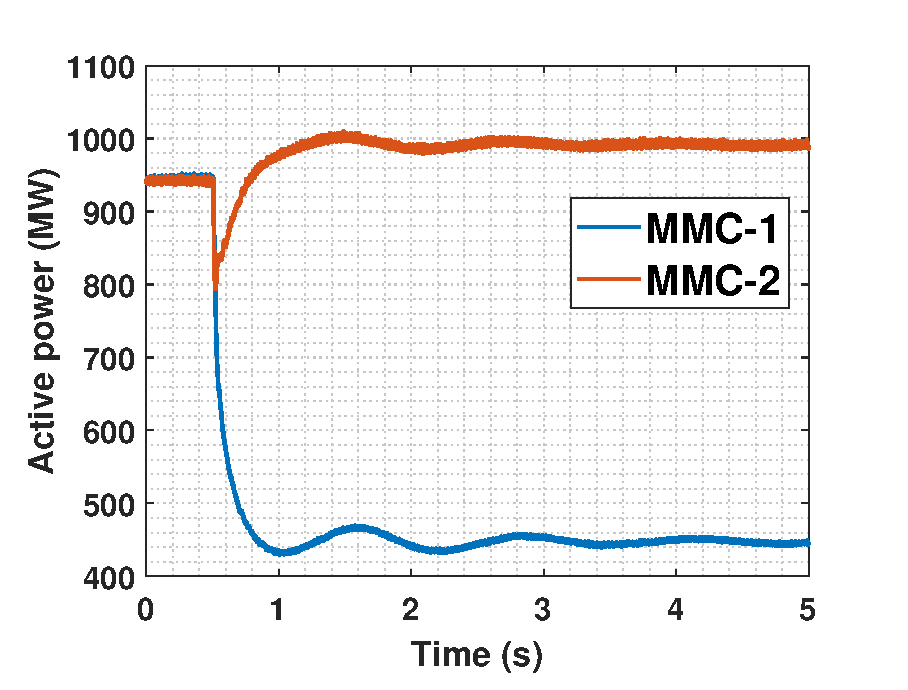
\includegraphics[height = 7cm,width = \textwidth]{Diagrams/Chapter_5/P_MMC_1_2_WT2off.eps}
    \caption{Active power in MMC-1 and MMC-2 buses upon OWF-2 disconnection event}
    \label{P_MMC_1_2_WT2off}
\end{figure}

\begin{figure}[H]
%\centering
%\hspace*{-1cm}
\subfloat[Currents in MMC-1 bus]{%
  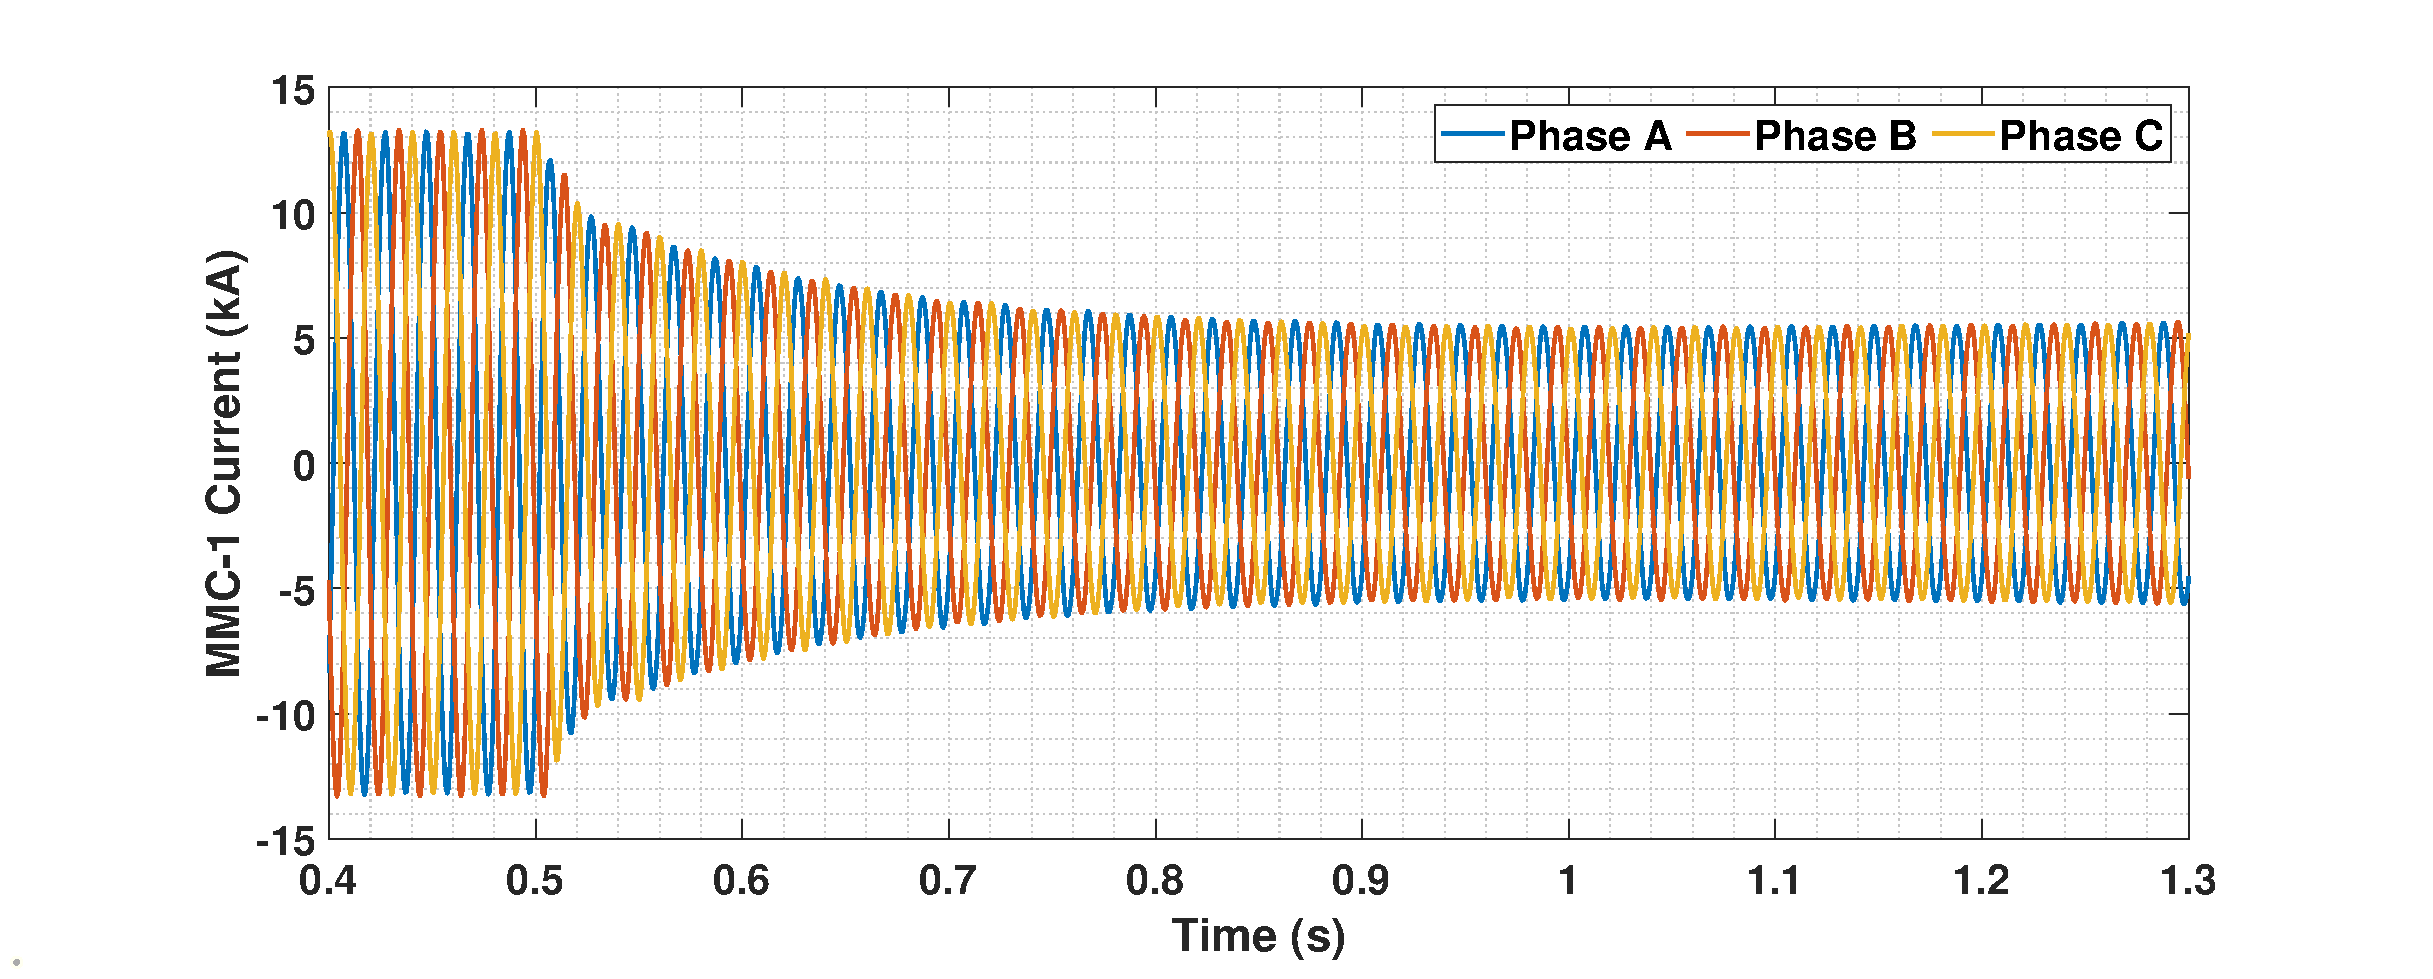
\includegraphics[height = 7cm,width = \textwidth]{Diagrams/Chapter_5/IABC_MMC_1_WT2off.eps}%
\label{fig:IABC_MMC_1_WT2off}}

%\hspace*{-1cm}
\subfloat[Currents in MMC-2 bus]{%
  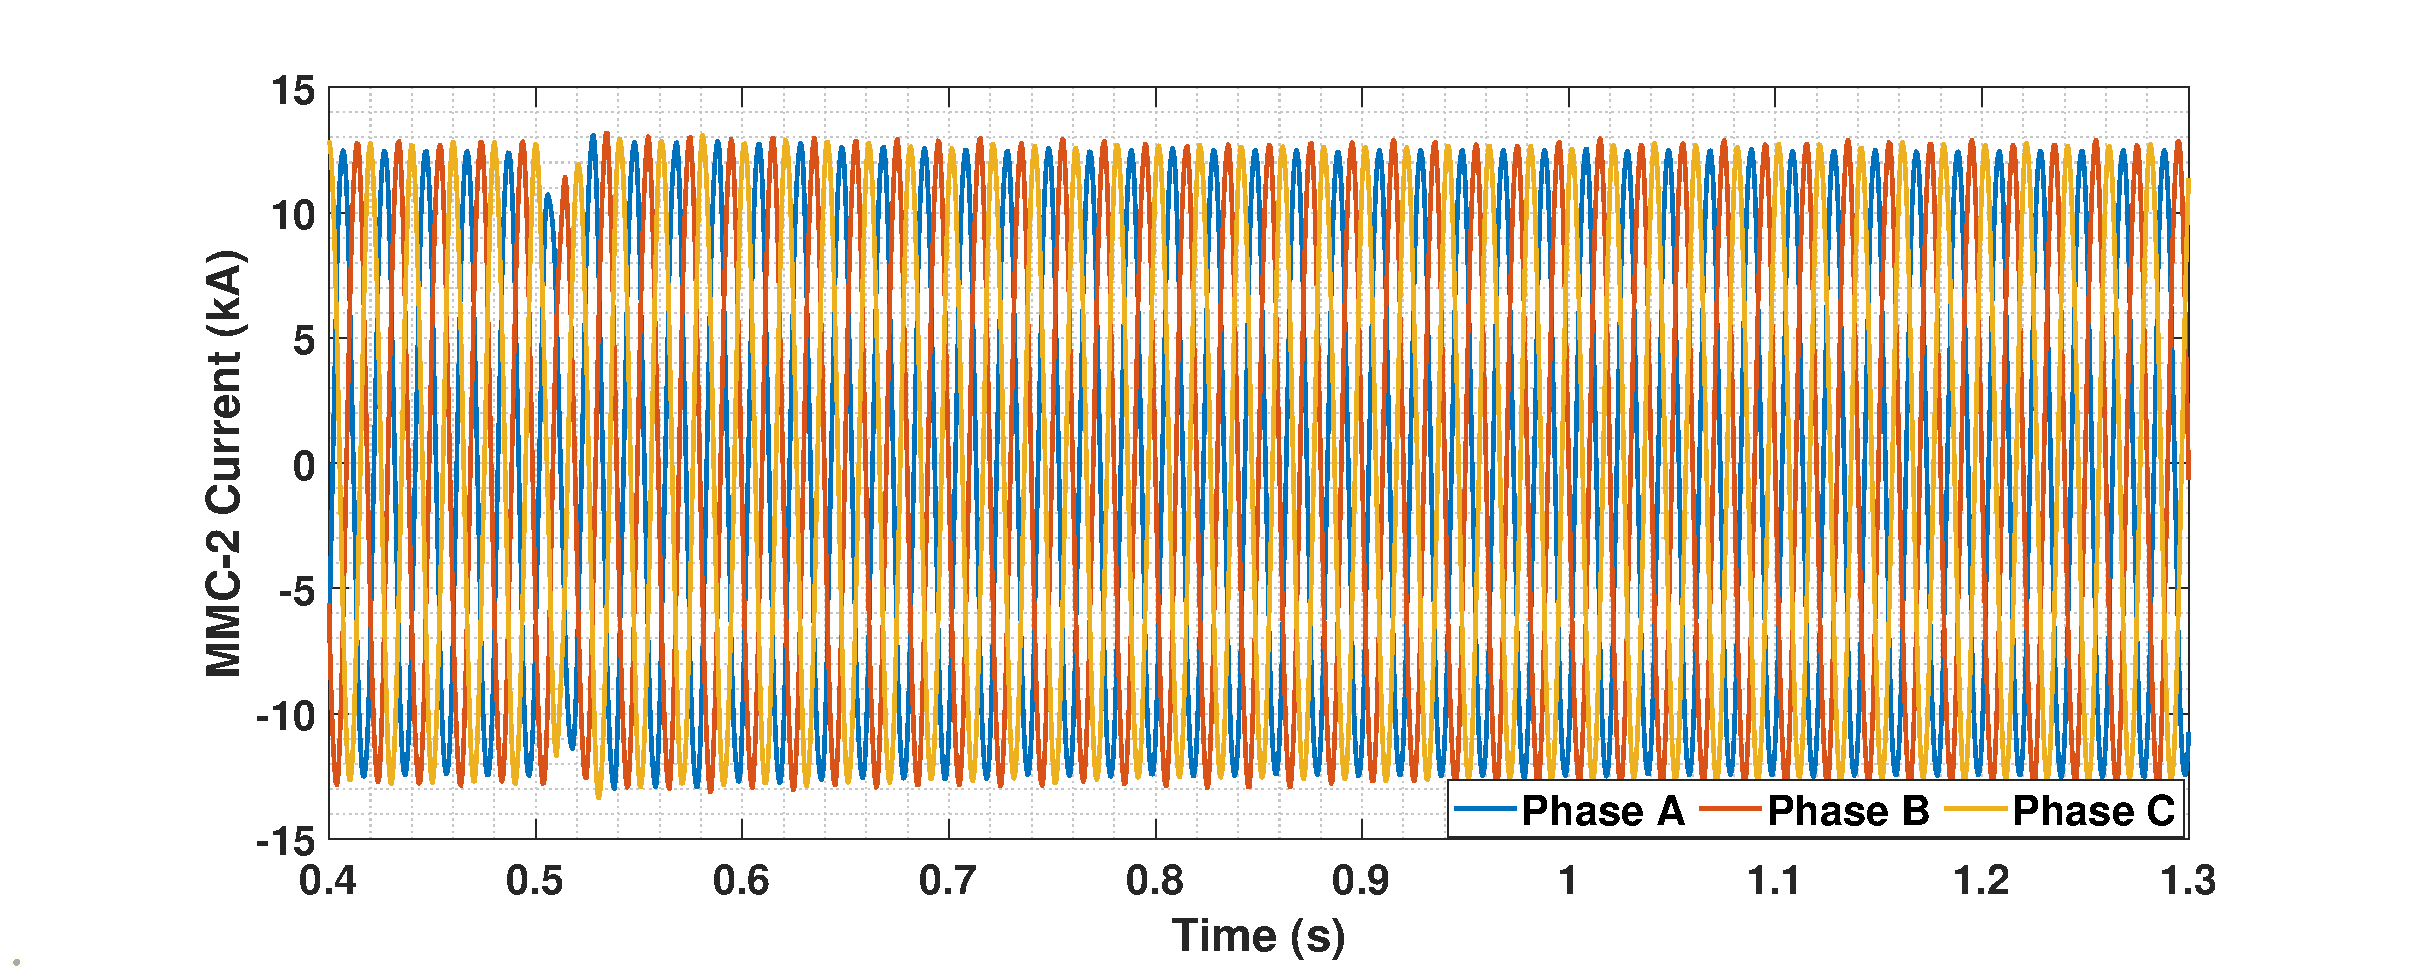
\includegraphics[height = 7cm,width = \textwidth]{Diagrams/Chapter_5/IABC_MMC_2_WT2off.eps}%
\label{fig:IABC_MMC_2_WT2off}}

\caption{Currents in a) MMC-1 bus and b) MMC-2 bus upon OWF-2 disconnection event}
\label{fig:IABC_MMC_1_2_WT2off}
\end{figure}


In the \gls{OWF}s side, the voltage at \gls{PCC}-2 goes beyond bounds and is in the condition as before energizing. This can be observed from the voltage in p.u. graph in Figure \ref{VACP_WT134_WT2off}b). During the disconnection of \gls{OWF}-2, there occurs a drop in voltage at \gls{PCC}-1, 3 and 4 as seen from the voltage graphs in Figure \ref{VACP_WT134_WT2off}a), c) and d). This happens since they are all connected to a common bus (\gls{MMC} bus). Moreover, in the post-fault period, voltages at \gls{PCC}-1, 3 and 4 are stabilized and settle to a higher value (nearly 1.08 p.u.) than the pre-fault voltage to compensate for the loss of \gls{OWF}-2. This is due to the fast local voltage control in the \gls{DVC} of the \gls{WG}s. But the currents at these \gls{OWF}s remain the same since the scaling factor for each \gls{OWF} is still 83 (83 $\times$ 6 MW = 498 MW). This can be viewed from the current measured at \gls{PCC}-1 in Figure \ref{IABC_WT1_WT2off}. Similar is the case for \gls{PCC}-3 and \gls{PCC}-4 and the graphs are shown in Appendix \ref{disconn_owf2_appen}. As voltage increases and current remains the same, the active power generated from the \gls{OWF}- 1, 3 and 4 increases and therefore the power flowing through \gls{MMC}-2 also increases.

\begin{figure}[H]
%\centering
\hspace*{-1.7cm}
    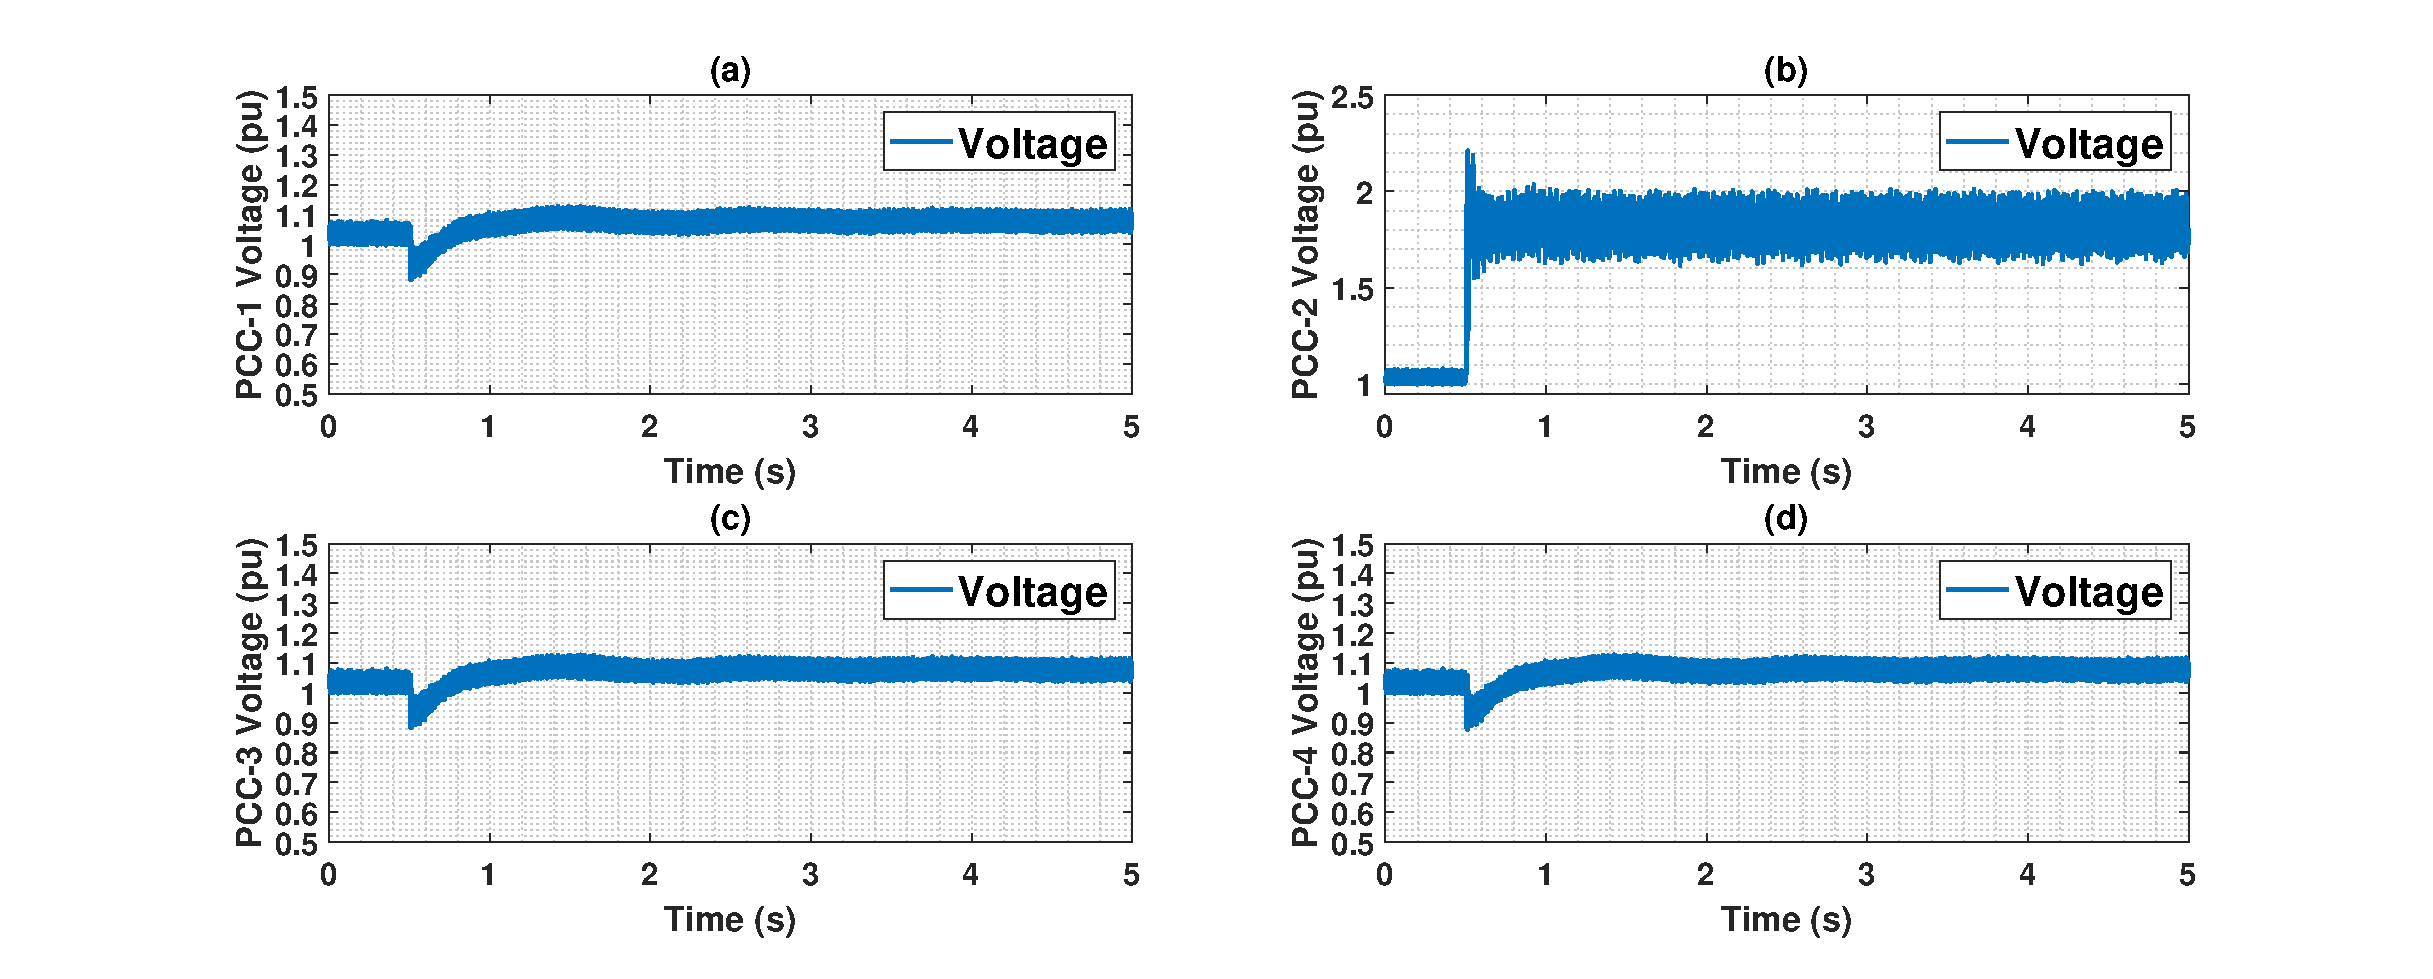
\includegraphics[height = 10.5cm,width = 20.5cm]{Diagrams/Chapter_5/VACP_WT1234_WT2off.eps}
    \caption{Voltage in p.u. at a) PCC-1, b) PCC-2, c) PCC-3 and d) PCC-4 upon OWF-2 disconnection event}
    \label{VACP_WT134_WT2off}
\end{figure}

\begin{figure}[H]
%\centering
%\hspace*{-1.2cm}
    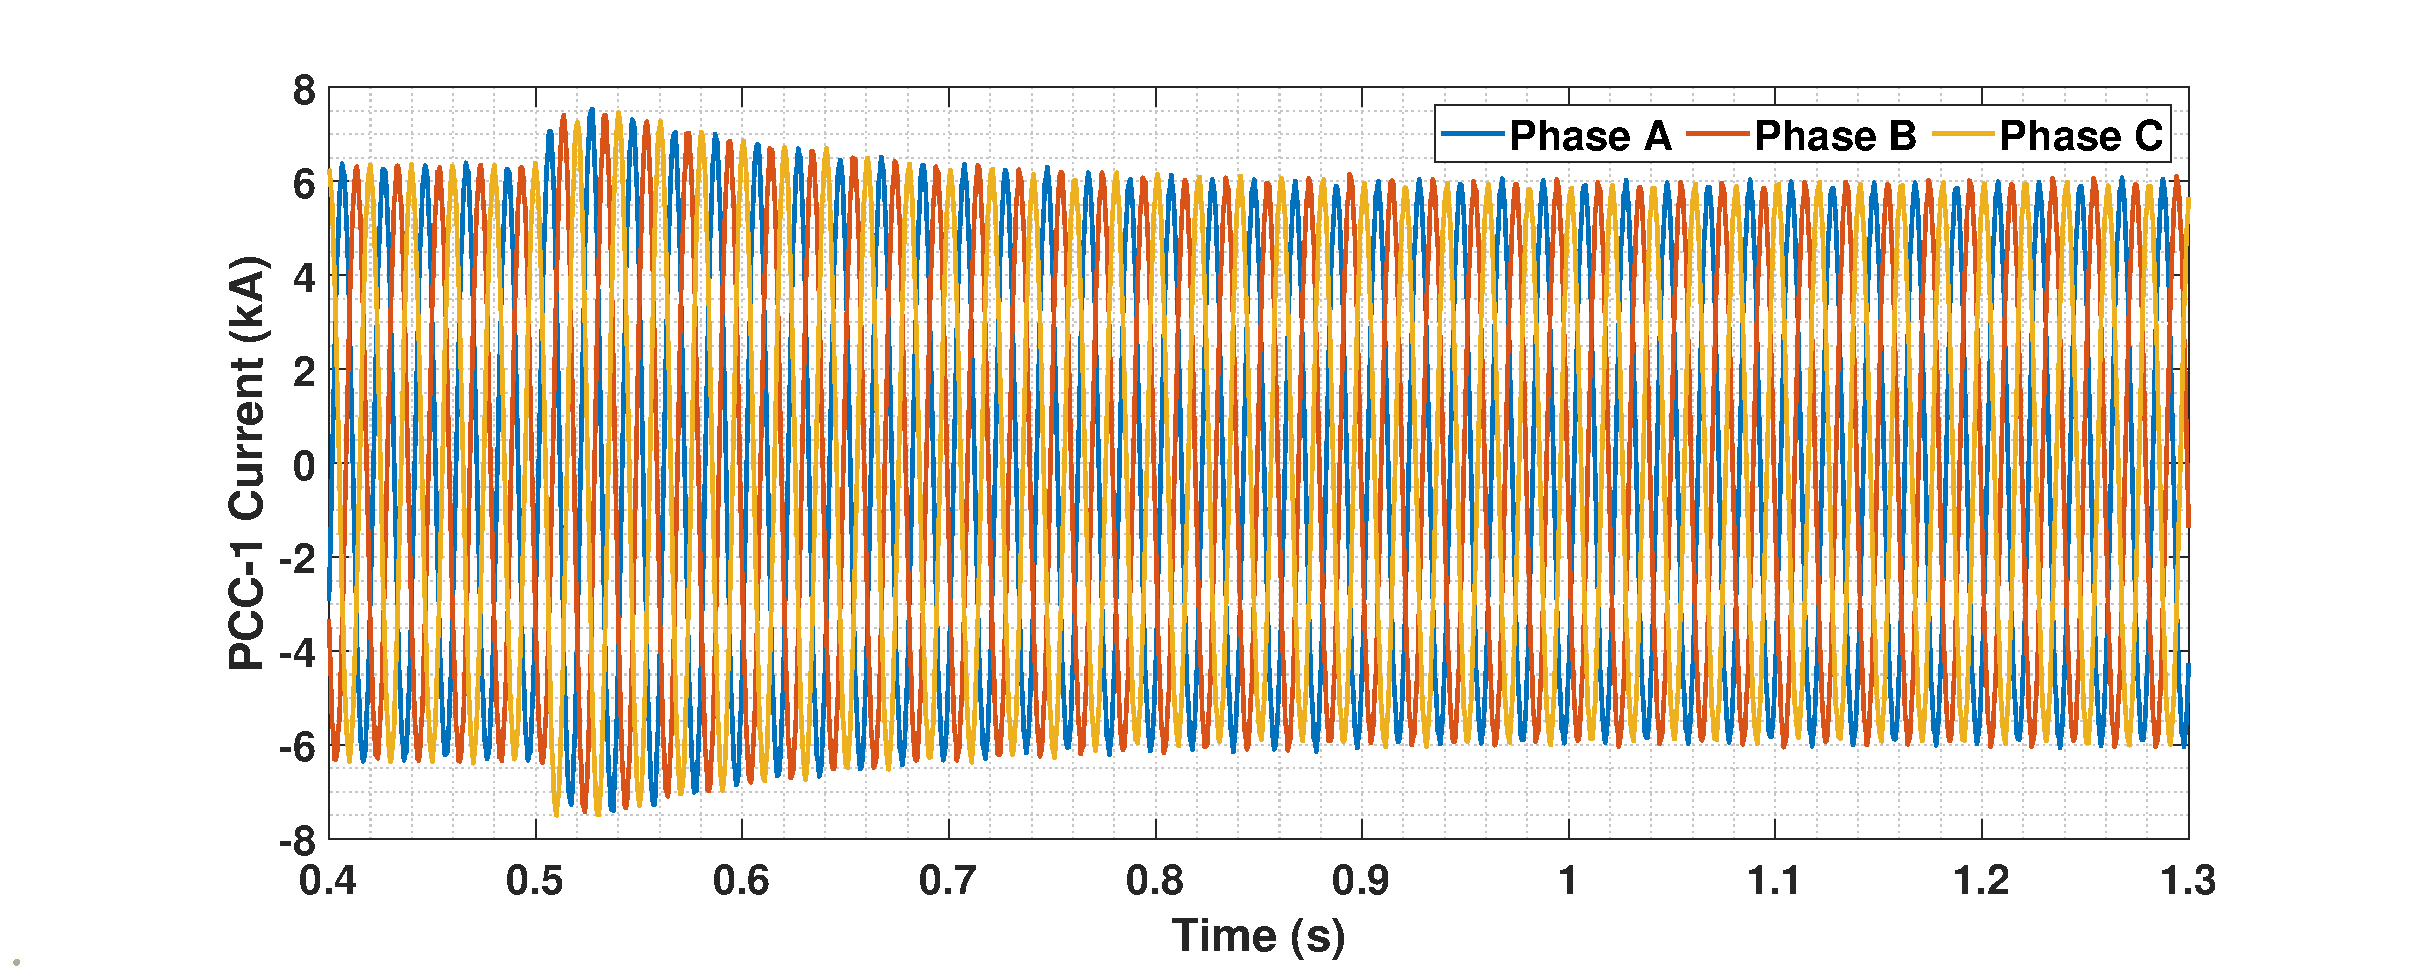
\includegraphics[height = 7cm,width = \textwidth]{Diagrams/Chapter_5/IABC_WT1_WT2off.eps}
    \caption{Currents at PCC-1 upon OWF-2 disconnection event}
    \label{IABC_WT1_WT2off}
\end{figure}

\subsection{Three-phase Line to Ground Fault}

Before the application of three-phase line to ground fault, a logic to operate the circuit breaker (CB-1a) at the cable-1 end is developed as shown in Figure \ref{fig:Fault_logic}. This logic is inspired from the "Fault Control" model 
\footnote{Tutorial >> SAMPLES >> Mainstep >> Fault Control} available in RSCAD. 
For the fault, the line to ground fault component available in RSCAD library is used \cite{rtds_tech}.

\subsubsection{Circuit Breaker Operation Logic}\label{Fault logic and cb}
The logic is developed for the operation of the circuit breaker CB-1a in Figure \ref{fig:WT4_MMC2_Chap5} by detecting overcurrent. The signal 'SWD2A' is the signal for operating CB-1a. Initially, the breaker is closed during the energizing process using the switch 'CabMMC$\_$side'. Once the system is fully operational after connecting all the four \gls{OWF}s and achieving 2 GW power in the network, the 'Activ' switch in Figure \ref{fig:Fault_logic} is turned on. This is done to provide the switching operation of CB-1a by comparing the RMS current ($I_{rms}$) and the maximum phase current ($I_{phase\_max}$)\footnote{$I_{phase\_max}$ = 10 \% above $I_{phase}$ = 1.1 $\times$ $I_{phase}$

$I_{phase}$ = $\frac{Apparent \;\; power \;\; in \;\; single-phase}{Line \;\; to \;\; neutral \;\; voltage}$} at CB-1a. The system is still in steady state condition. Once the fault is applied, when $I_{rms}$ becomes greater than $I_{phase\_max}$, the SR flip flop detects the change and holds a value of zero for the signal 'SWD2A'. This action causes the breaker CB-1a to open. The delay block before the signal 'SWD2A' provides time delay for the operation of circuit breaker after the fault has been detected.

\begin{figure}[H]
\centering
%\hspace*{-1.2cm}
    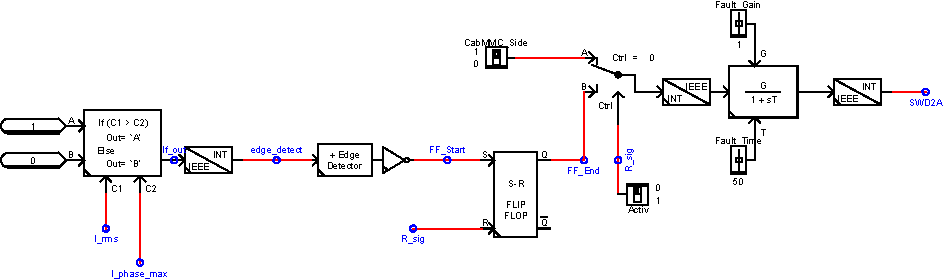
\includegraphics[height = 4.5cm,width = \textwidth]{Diagrams/Chapter_5/Fault_logic_New.pdf}
    \caption{Circuit breaker operation logic}
    \label{fig:Fault_logic}
\end{figure}

\begin{figure}[H]
%\centering
%\hspace*{-1.2cm}
    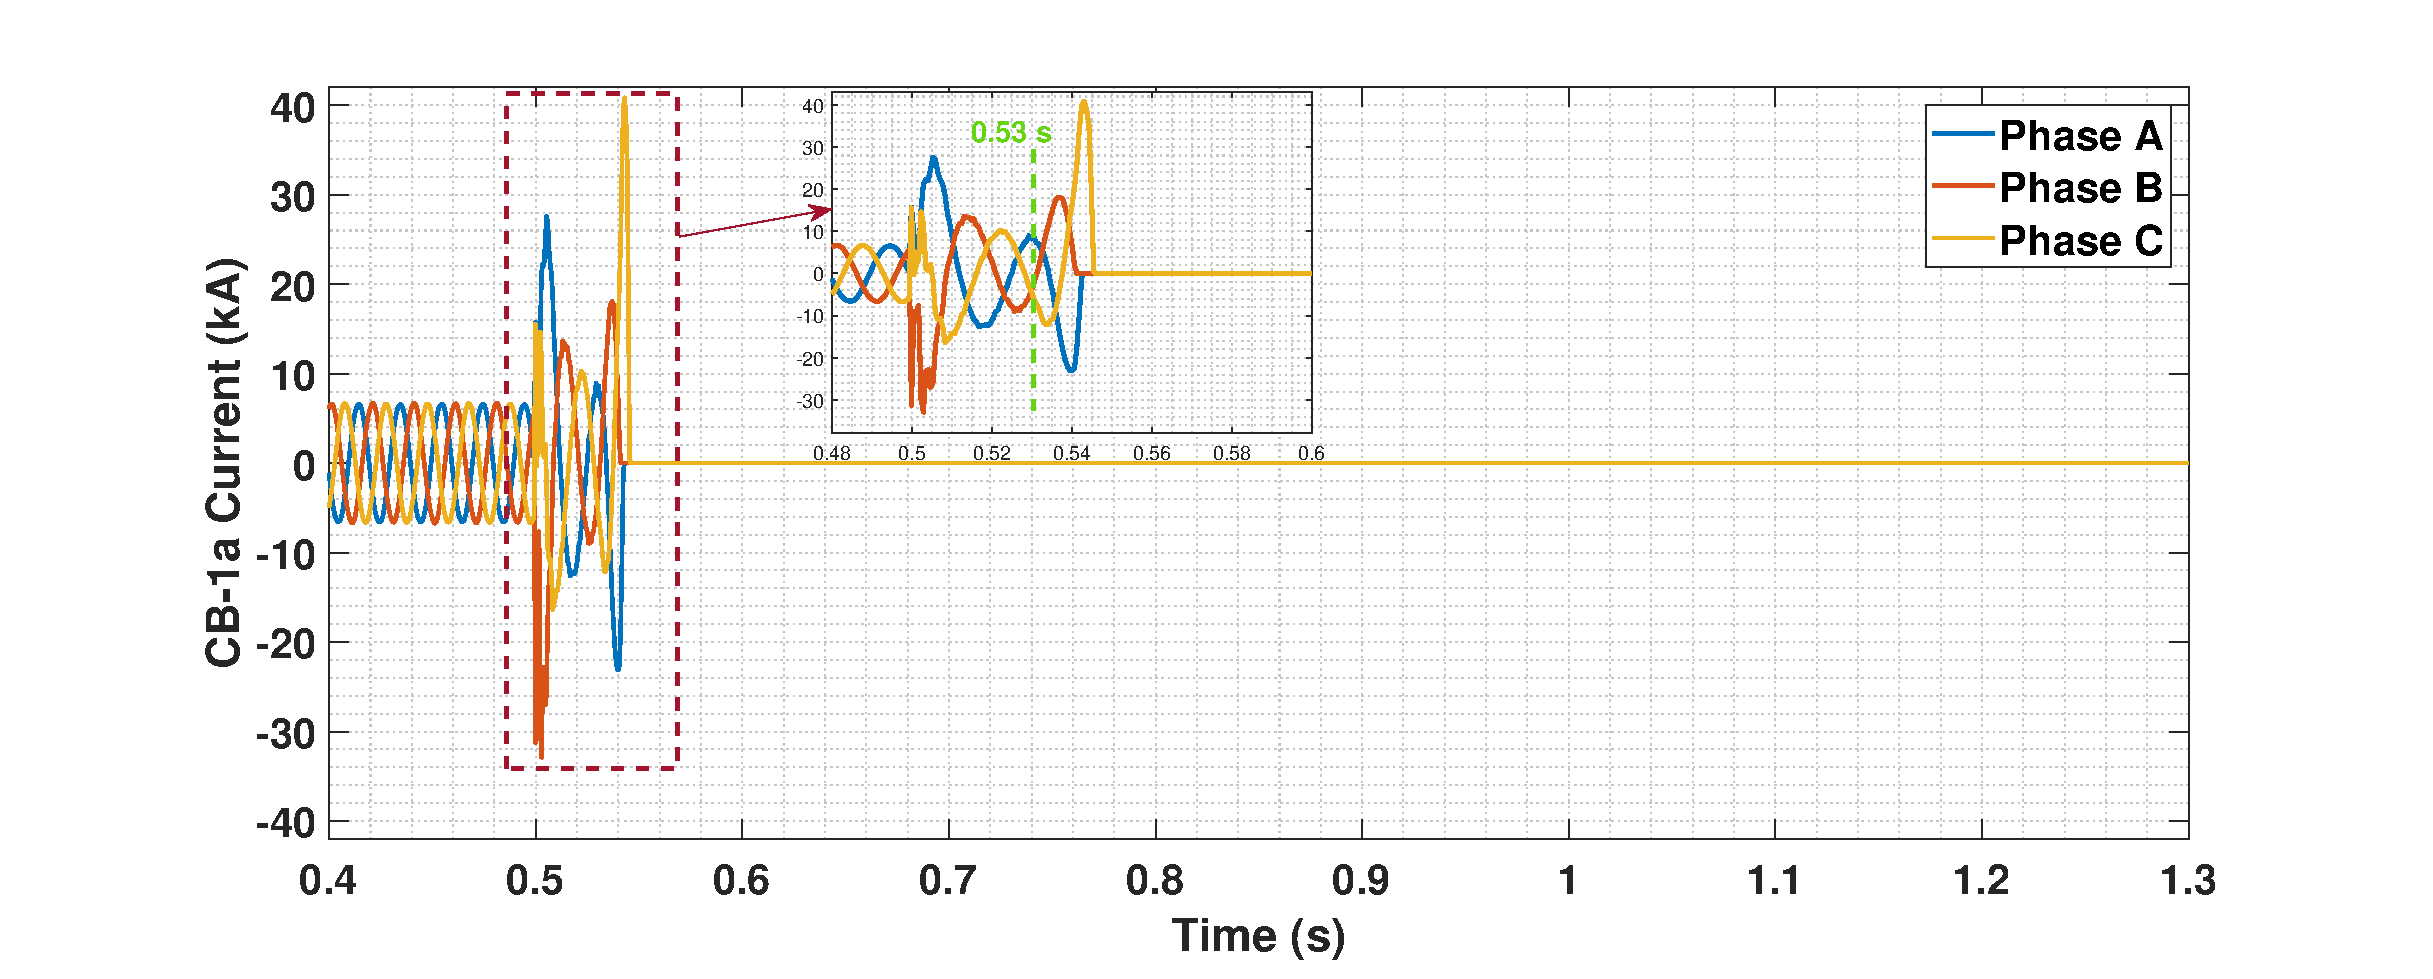
\includegraphics[height = 7.5cm,width = \textwidth]{Diagrams/Chapter_5/IABC_CB_3phaseSC_new_5.eps}
    \caption{Currents in circuit breaker (CB-1a) upon three-phase line to ground fault in the middle of cable-1}
    \label{Circuit_breaker_3phasefault}
\end{figure}

In order to analyze the short-term voltage stability of the system, a permanent three-phase line to ground fault is applied in the middle of \gls{HVAC} cable-1. The response of the network is recorded, and the plots for voltages, currents, active and reactive powers are depicted from Figure \ref{Circuit_breaker_3phasefault} to Figure \ref{IDQ_WT1_3phaseSC} for the event. During the time of the fault, the RMS current exceeds the maximum phase current and the logic developed detects this overcurrent at CB-1a. This leads to the opening of breaker CB-1a according to the logic explained in the previous paragraph. The overcurrent is detected at 0.53 s of the simulation from the developed logic. A short delay of nearly 12 ms is provided to open the breaker after the fault has been detected similar to a practical scenario (Figure \ref{Circuit_breaker_3phasefault}). After the circuit breaker is opened, \gls{OWF}-1 is isolated from the network and total power provided to the onshore system is reduced. The total power in the pre-fault period is nearly 2 GW, and after the fault, the total power is reduced to nearly 1500 MW. Similar to the disconnection of one \gls{OWF} discussed earlier in Section \ref{disconnection_one_OWF}, the power flow is reduced through \gls{MMC}-1 as shown by the blue line in Figure \ref{17_3phaseSC}. It is also worthy of mentioning that the network is stable by viewing the stable voltage in the post-fault period in \gls{MMC} bus, as shown in Figure \ref{VABC_MMC_1_3phaseSC}.



Increase in active power in \gls{MMC}-2 after the fault has been cleared (as seen from the red line in Figure \ref{17_3phaseSC}) can be explained by viewing the current profiles in the \gls{OWF}s detailed in the following paragraph. A major observation can be viewed from the profile of transients during the fault in the currents of both the \gls{MMC}s in Figure \ref{fig:IABC_MMC_1_3phaseSC} and \ref{fig:IABC_MMC_2_3phaseSC}. The initial rise in current till 0.53 s is due to the occurrence of the three-phase fault. The breaker is opened at 0.542 s. The profile of currents at nearly 0.59 s are complementary in both \gls{MMC}s, i.e. the currents are decreasing in \gls{MMC}-1 and increasing in \gls{MMC}-2. This is due to the difference in control strategies in \gls{MMC}-1 (V/F control) and \gls{MMC}-2 (active power control).

\begin{figure}[H]
%\centering
%\hspace*{-1.2cm}
    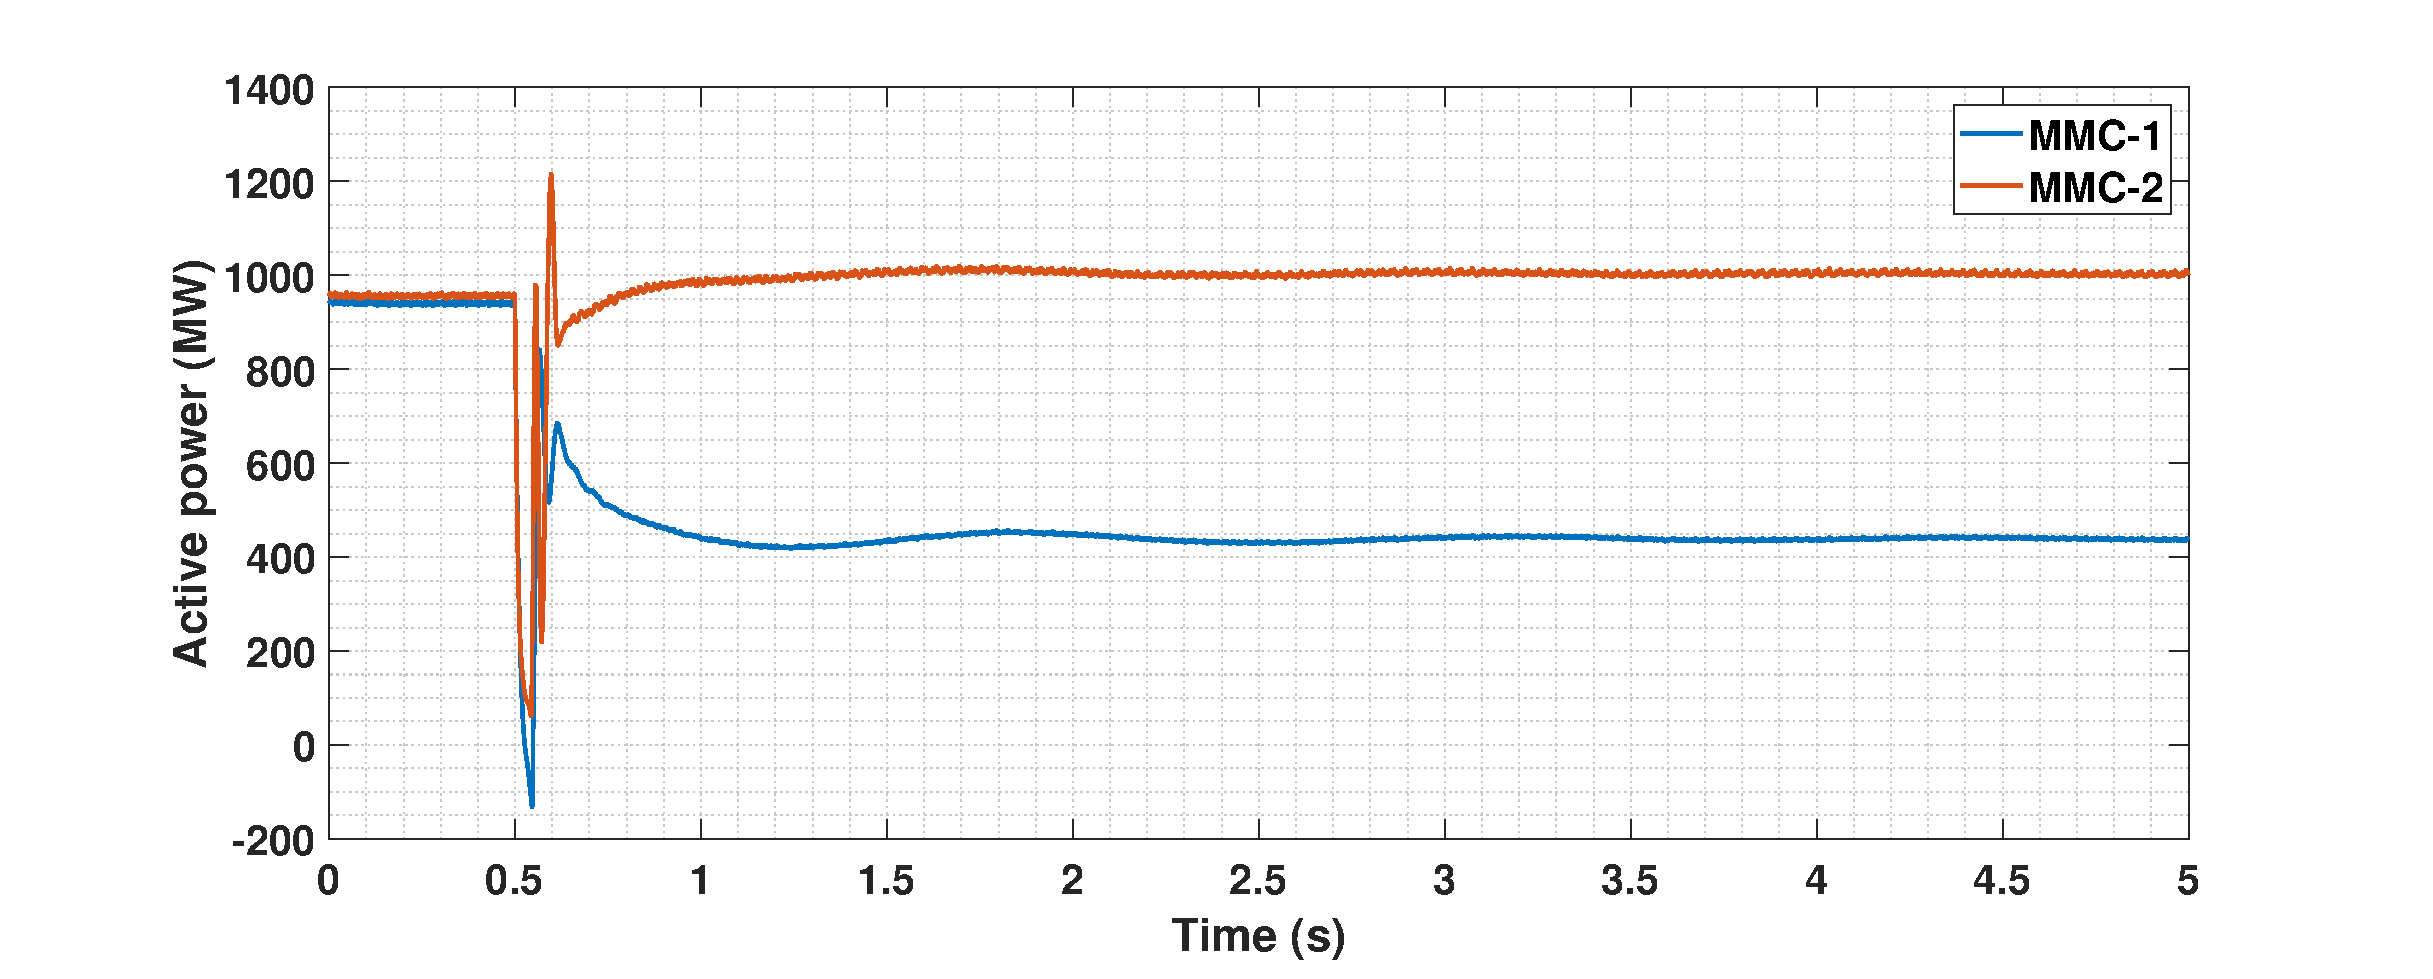
\includegraphics[height = 7cm,width = \textwidth]{Diagrams/Chapter_5/P_MMC_1_2_3phaseSC.eps}
    \caption{Active power in MMC-1 bus and MMC-2 bus upon three-phase line to ground fault in the middle of cable-1}
    \label{17_3phaseSC}
\end{figure}

\begin{figure}[H]
%\centering
%\hspace*{-1.2cm}
    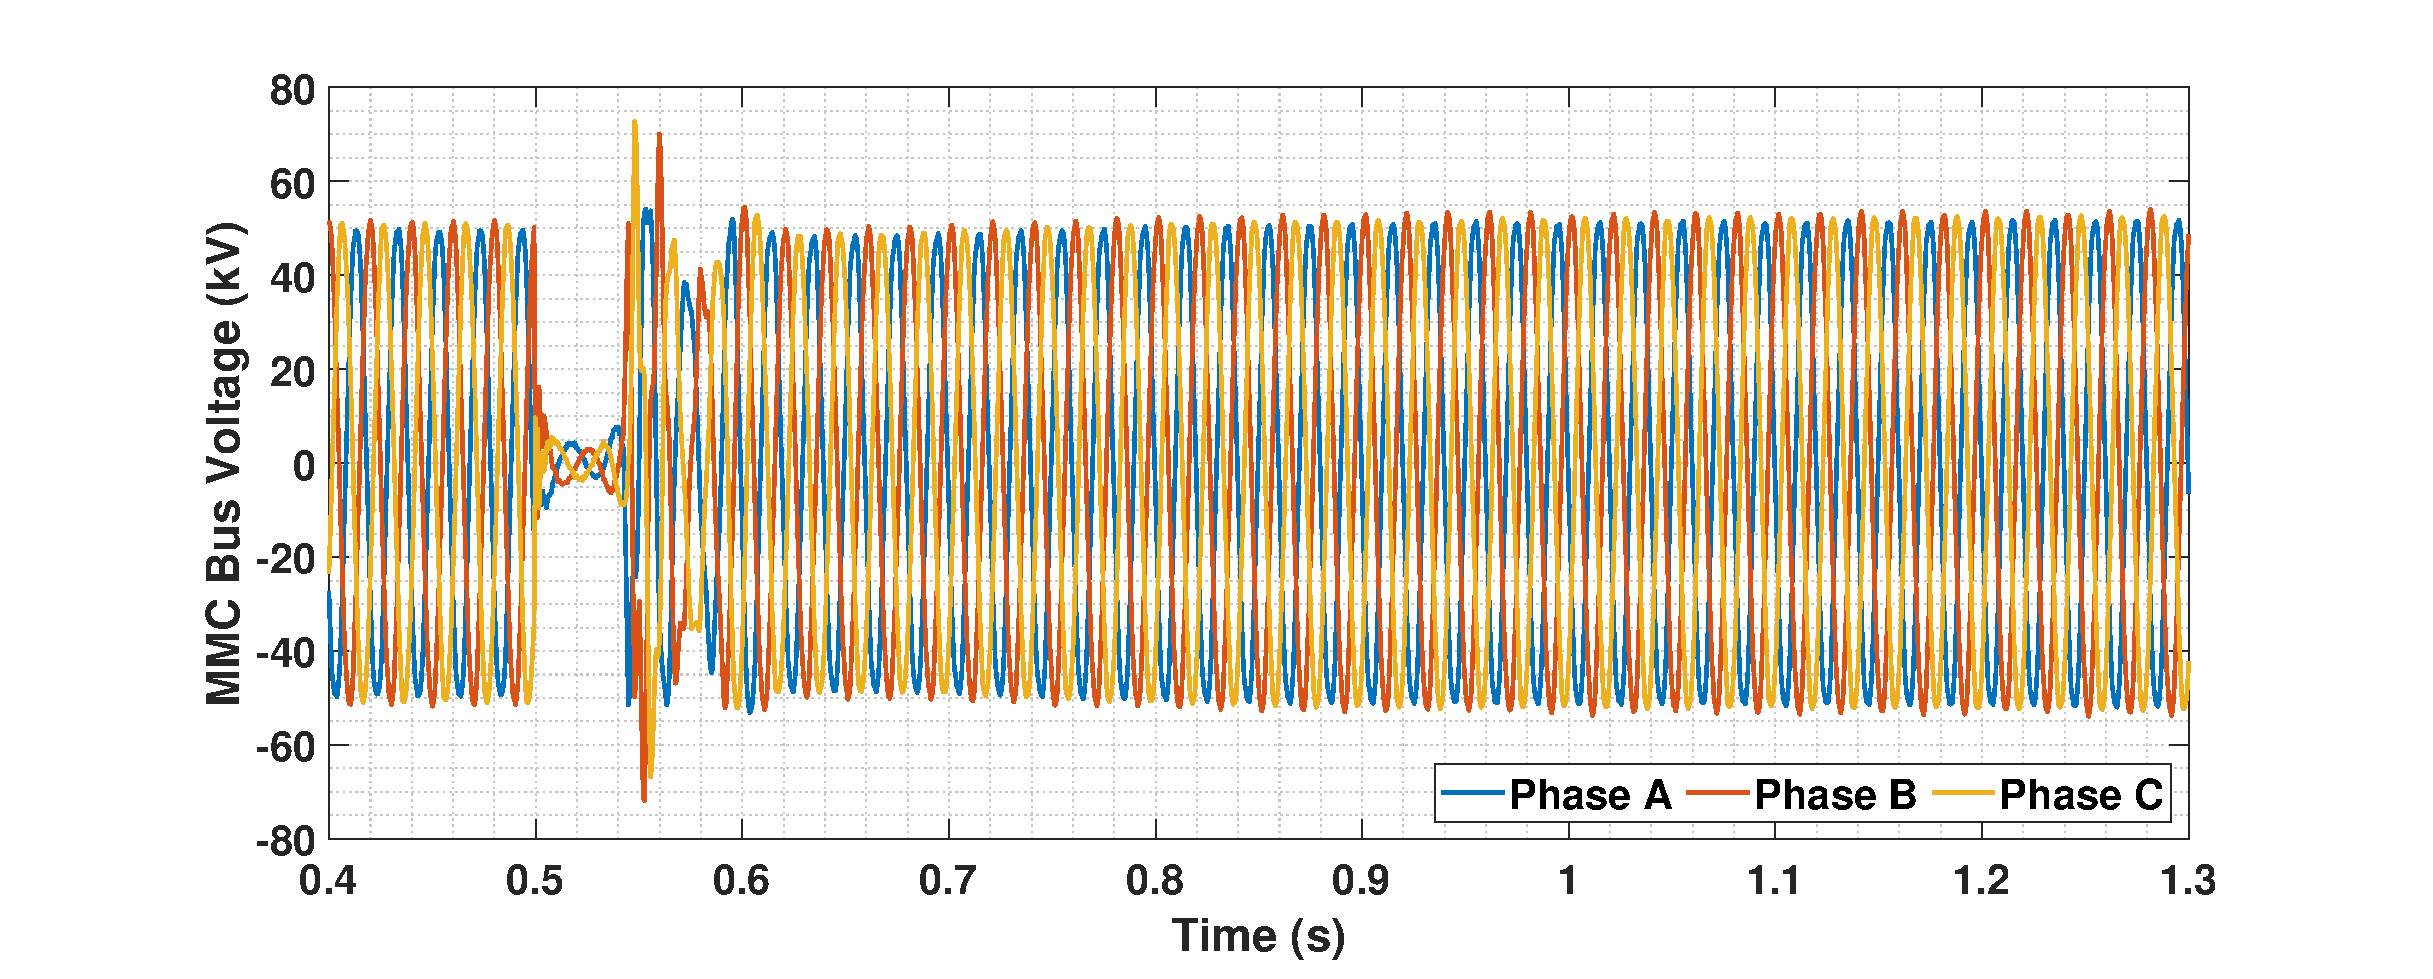
\includegraphics[height = 7cm,width = \textwidth]{Diagrams/Chapter_5/VABC_MMC_1_3phaseSC.eps}
    \caption{Voltages at MMC bus upon three-phase line to ground fault in the middle of cable-1}
    \label{VABC_MMC_1_3phaseSC}
\end{figure}


\begin{figure}[H]
%\centering
%\hspace*{-1.2cm}
\subfloat[Currents in MMC-1 bus]{%
  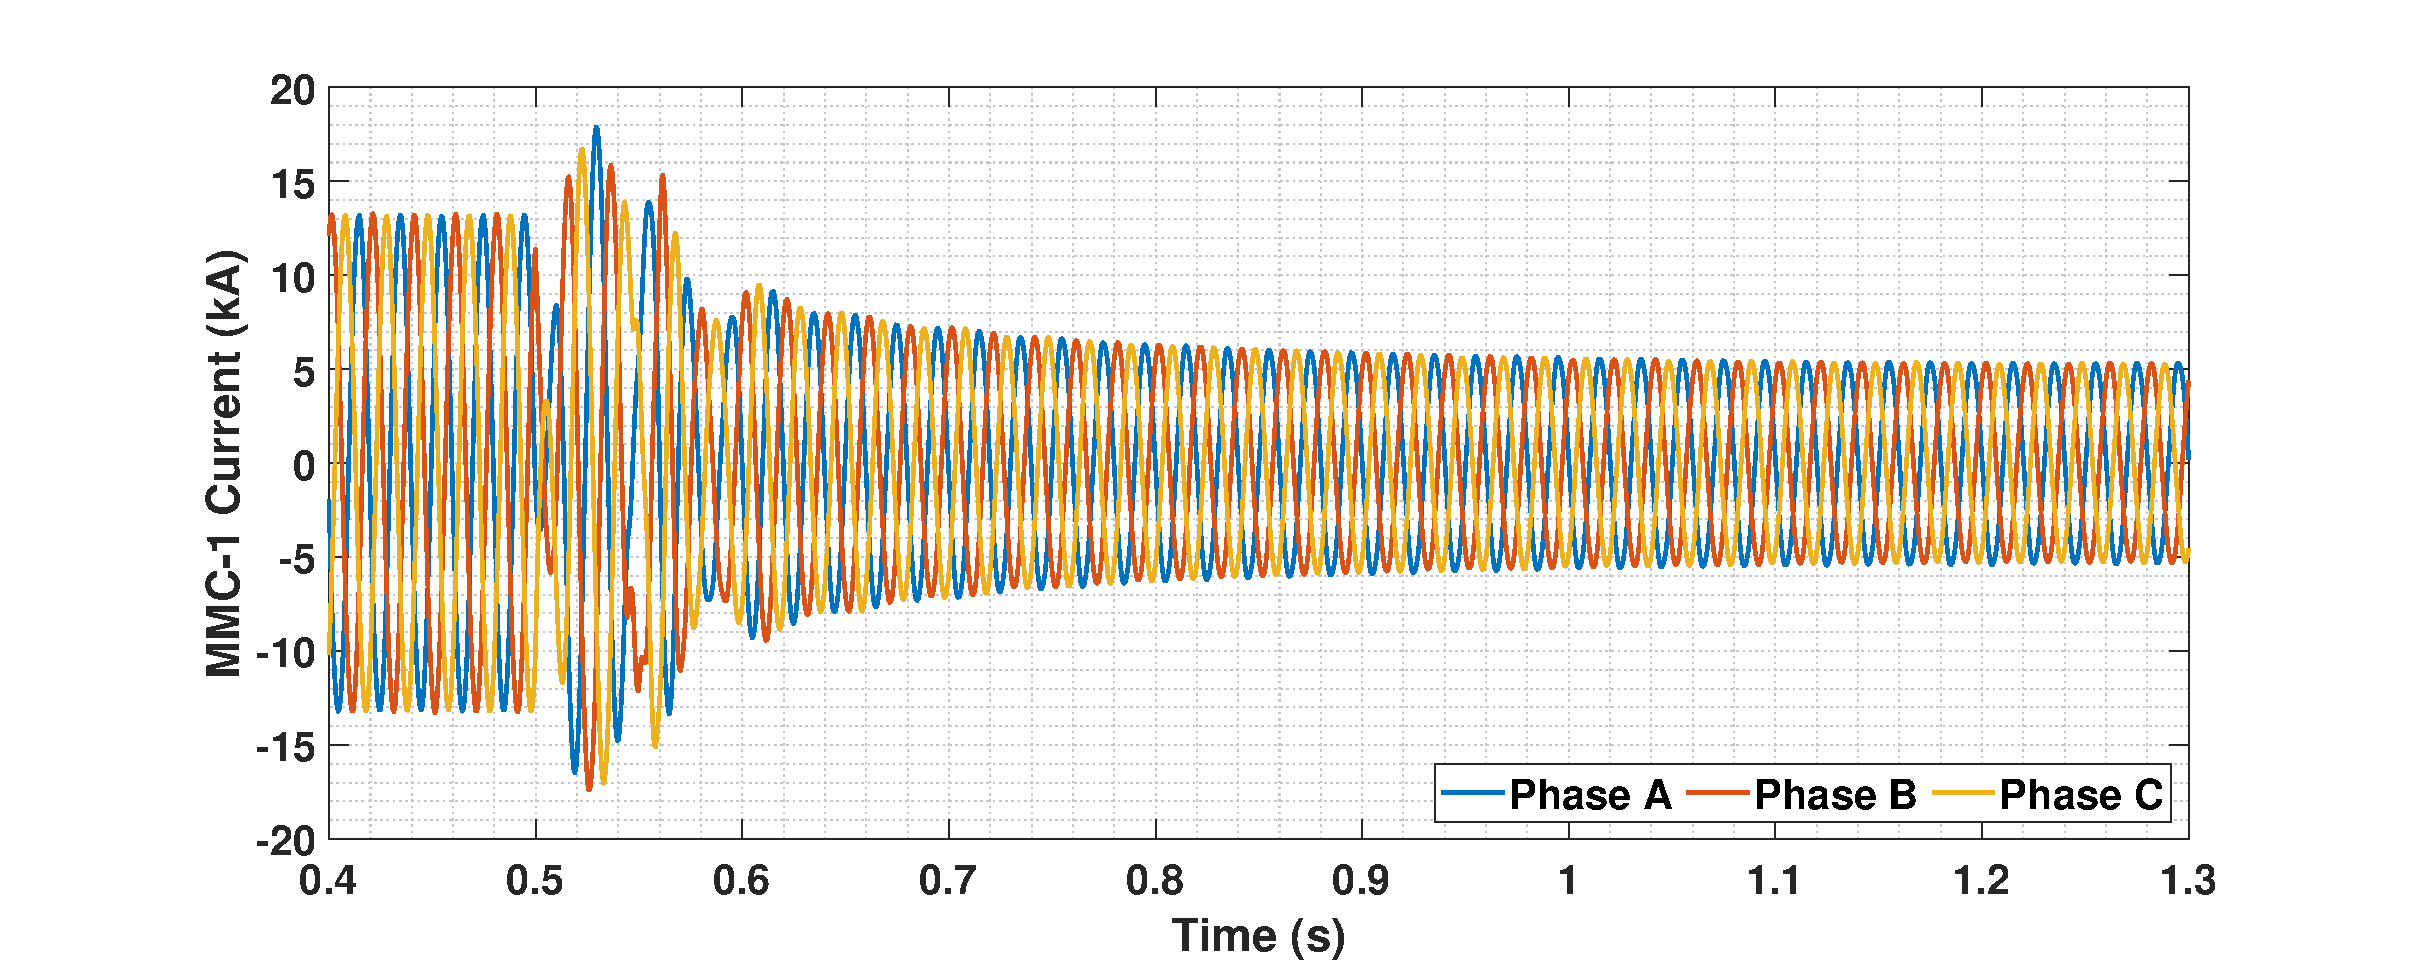
\includegraphics[height = 7cm,width = \textwidth]{Diagrams/Chapter_5/IABC_MMC_1_3phaseSC.eps}%
\label{fig:IABC_MMC_1_3phaseSC}}

%\hspace*{-1.2cm}
\subfloat[Currents in MMC-2 bus]{%
  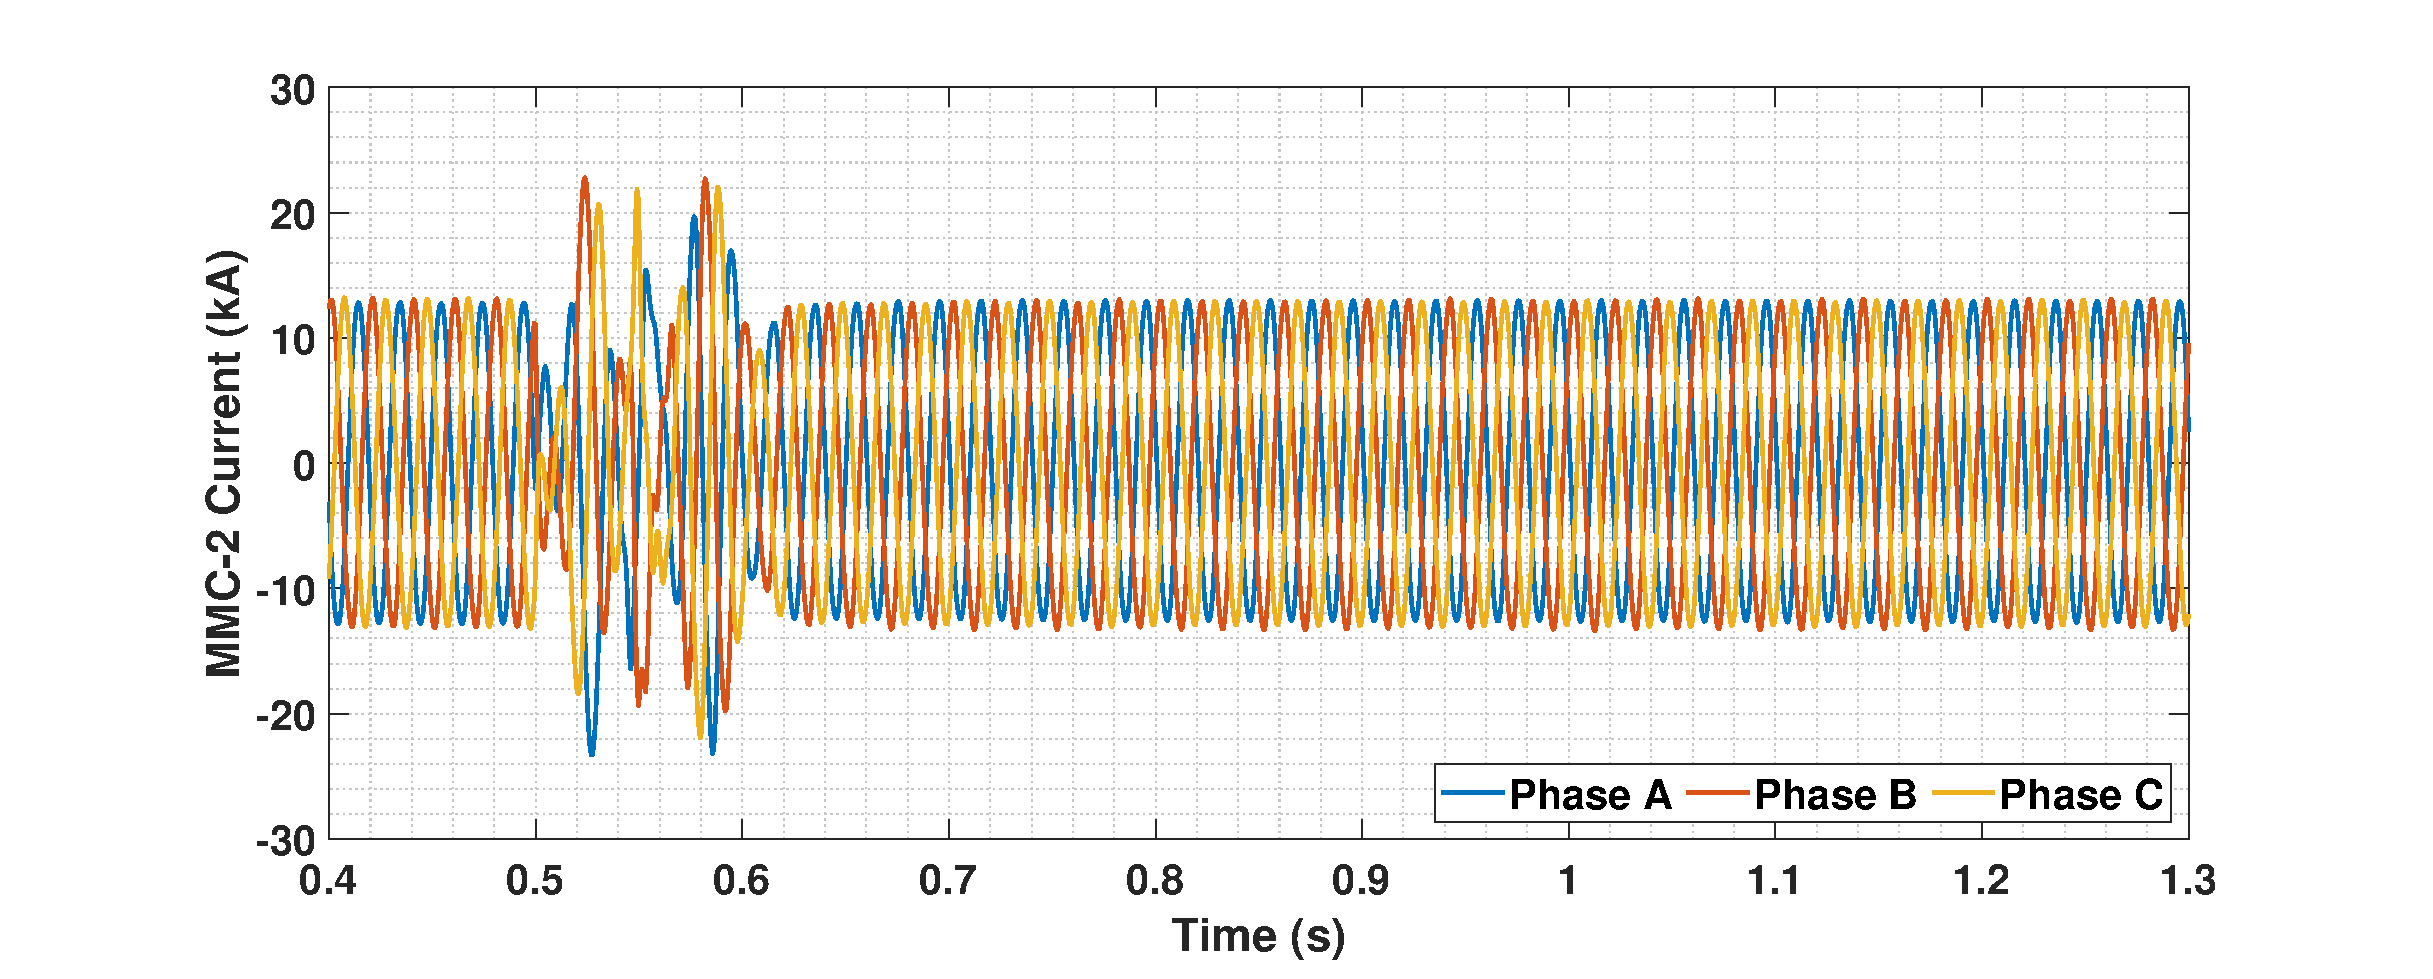
\includegraphics[height = 7cm,width = \textwidth]{Diagrams/Chapter_5/IABC_MMC_2_3phaseSC.eps}%
\label{fig:IABC_MMC_2_3phaseSC}}

\caption{Currents in a) MMC-1 bus and b) MMC-2 bus upon three-phase line to ground fault in the middle of cable-1}
\label{fig:IABC_MMC_1_2_3phaseSC}
\end{figure}

Analyzing at the \gls{OWF}s side of the network, the \gls{DVC} is modelled to provide rated reactive current to flow to the fault location by controlling the voltage of the \gls{GSC}, as explained in Section \ref{DVC_RSCAD}. From the voltage in p.u. plot in Figure \ref{VACP_WT1_3phaseSC} and the three-phase voltage plot in Figure \ref{VABC_WT1_3phaseSC}, it can be seen that the voltage at the \gls{PCC}-1 drops and remains low throughout the fault period. During the time of fault in cable-1 and after CB-1a is opened, the voltage angle and magnitude at \gls{PCC}-1 goes to zero. The \gls{PLL} in \gls{GSC}-1 is synchronized with the \gls{AC} voltage at \gls{PCC}-1. The voltage magnitude at \gls{GSC}-1 remains non-zero, and the voltage angle is zero during the time of fault as the \gls{PLL} follows the angular reference at \gls{PCC}-1. Therefore, due to higher voltage magnitude at \gls{GSC}-1 than at \gls{PCC}-1, reactive power will flow from \gls{GSC}-1 to \gls{PCC}-1, and since the voltage angle is zero at \gls{GSC}-1 and \gls{PCC}-1, active power transmitted is zero during the time of the fault. This is performed in \gls{DVC} by controlling the d-axis reference voltage of \gls{GSC}-1 and thereby indirectly controlling the current coming out of the \gls{GSC}-1 to \gls{PCC}-1. The current limitation algorithm implemented in the \gls{DVC} in Section \ref{currentlimitation_RSCAD}, limits the output current to the rating of the converter and hence rated reactive current flows from the \gls{GSC}-1 as seen in Figure \ref{WT1_currents_3phasefault}.



\begin{figure}[H]
%\centering
%\hspace*{-1.2cm}
    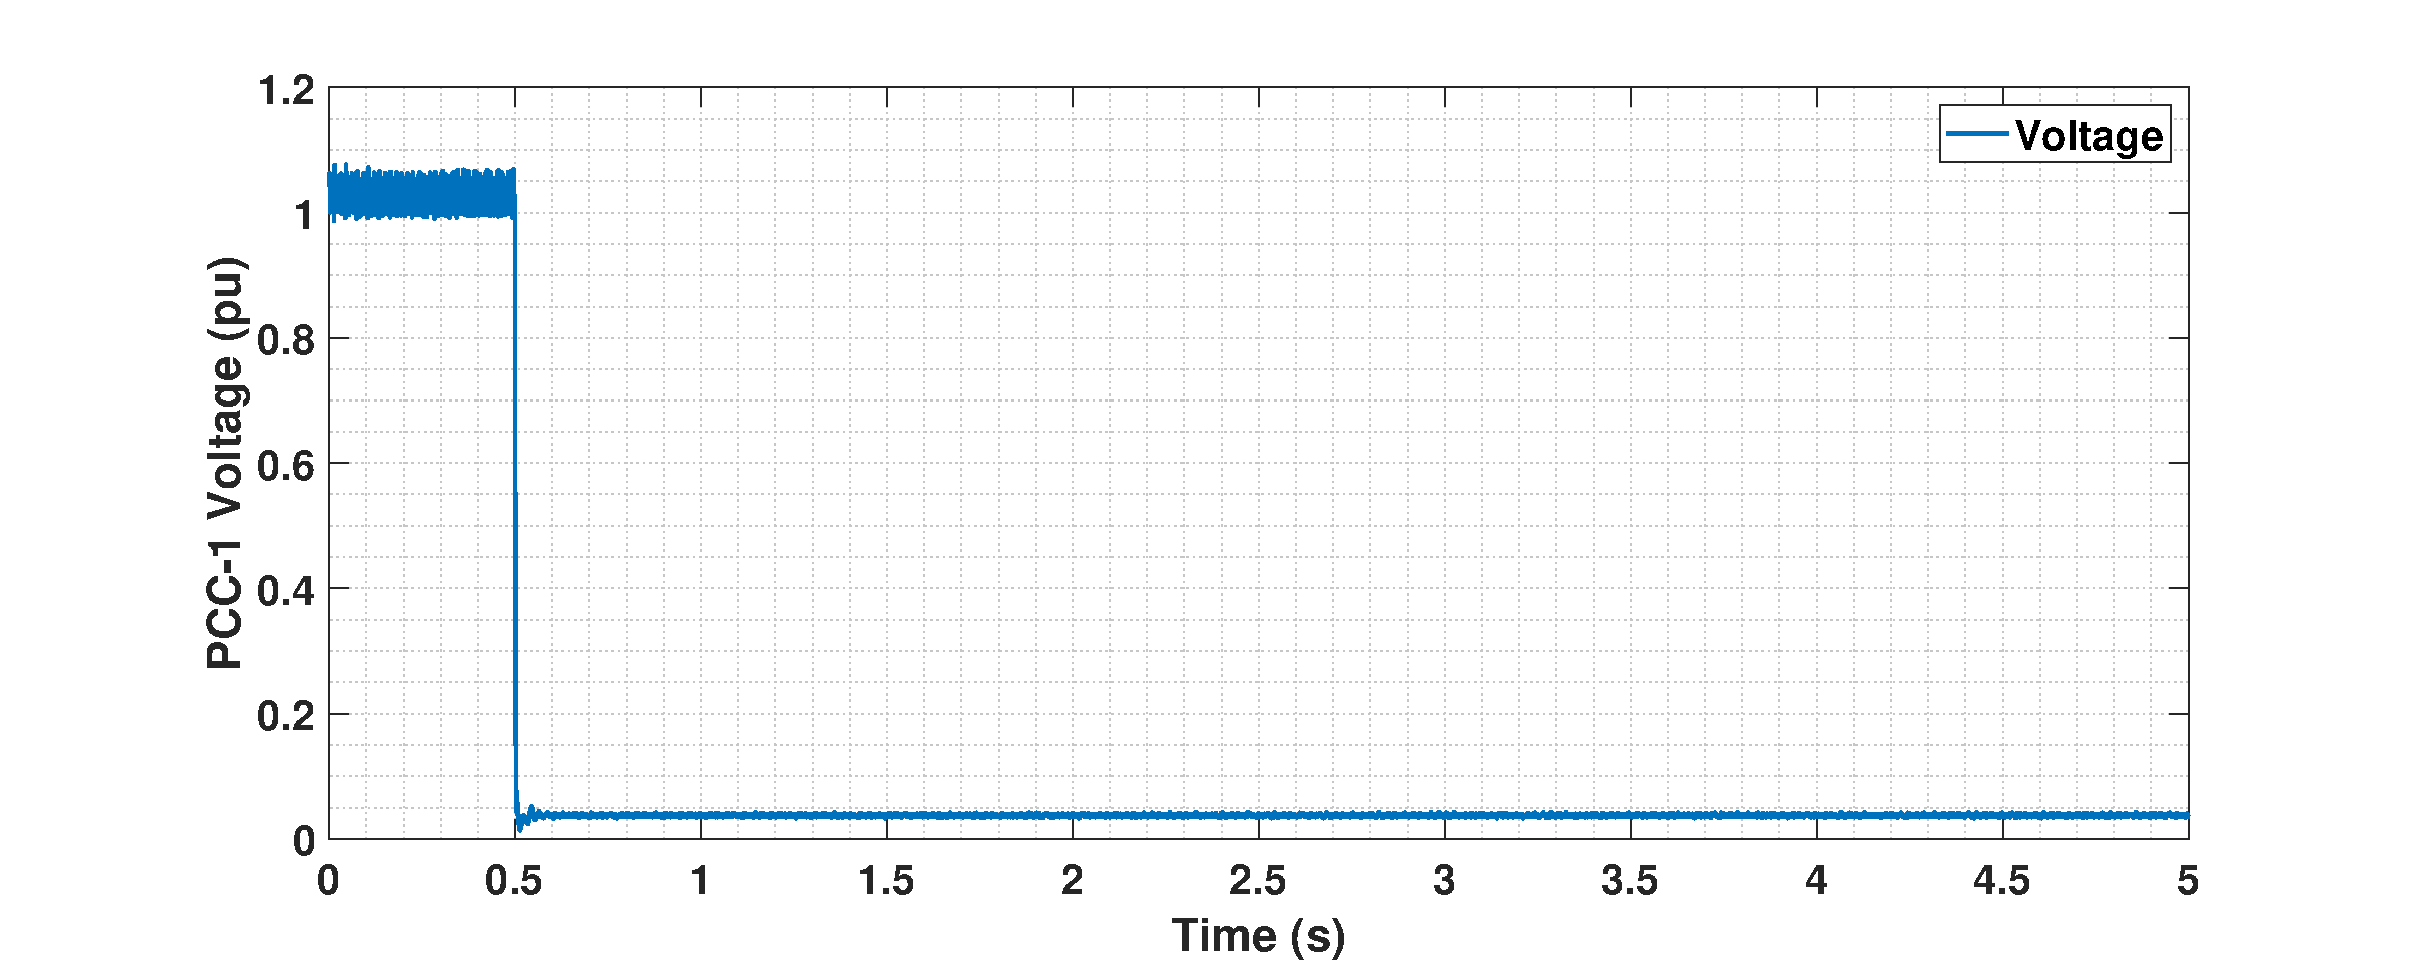
\includegraphics[height = 6.5cm,width = \textwidth]{Diagrams/Chapter_5/VACP_WT1_3phaseSC.eps}
    \caption{Voltage in p.u. at PCC-1 upon three-phase line to ground fault in the middle of cable-1}
    \label{VACP_WT1_3phaseSC}
\end{figure}

\begin{figure}[H]
%\centering
%\hspace*{-1.2cm}
    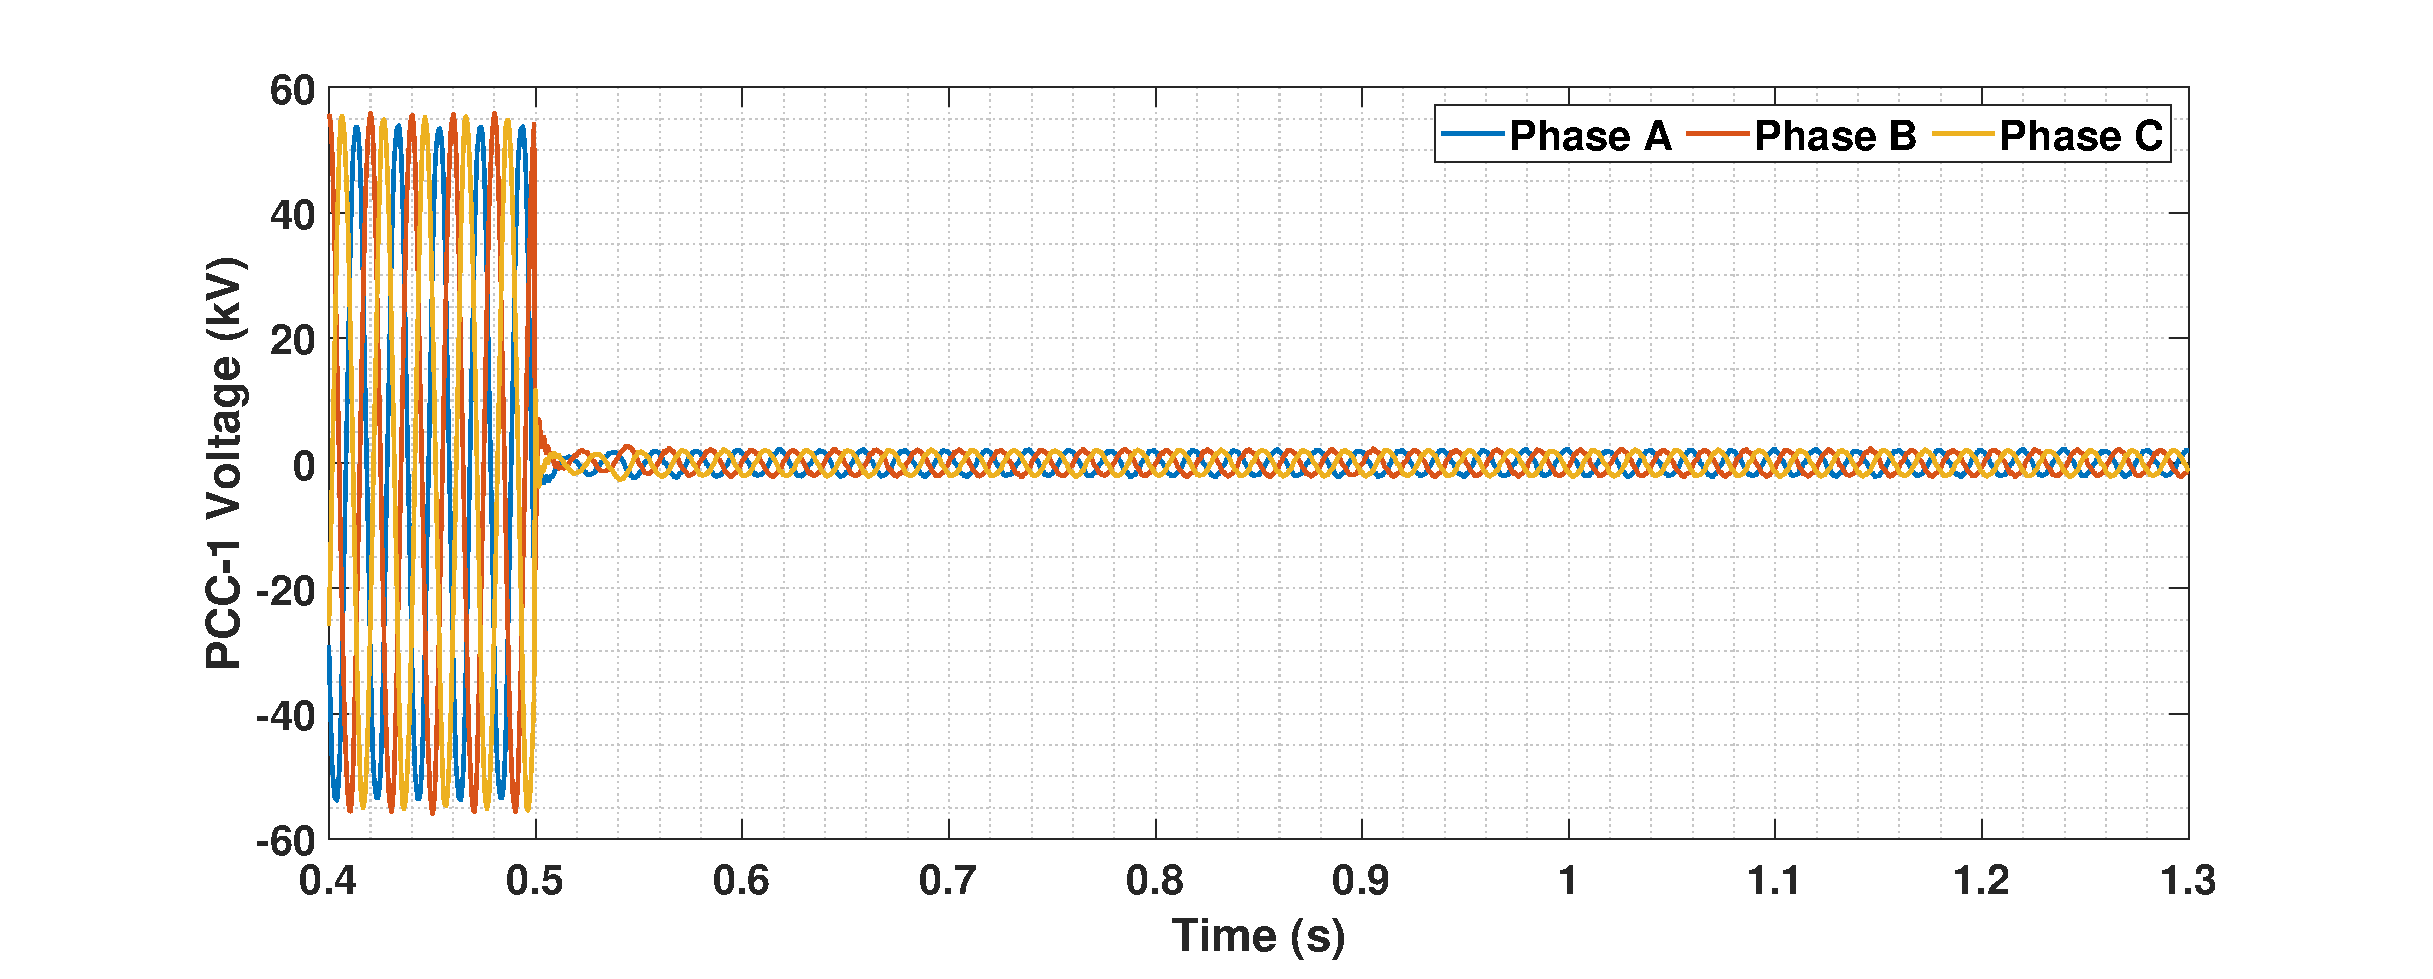
\includegraphics[height = 6.5cm,width = \textwidth]{Diagrams/Chapter_5/VABC_WT1_3phaseSC.eps}
    \caption{Voltages at PCC-1 upon three-phase line to ground fault in the middle of cable-1}
    \label{VABC_WT1_3phaseSC}
\end{figure}

\begin{figure}[H]
%\centering
%\hspace*{-1.2cm}
    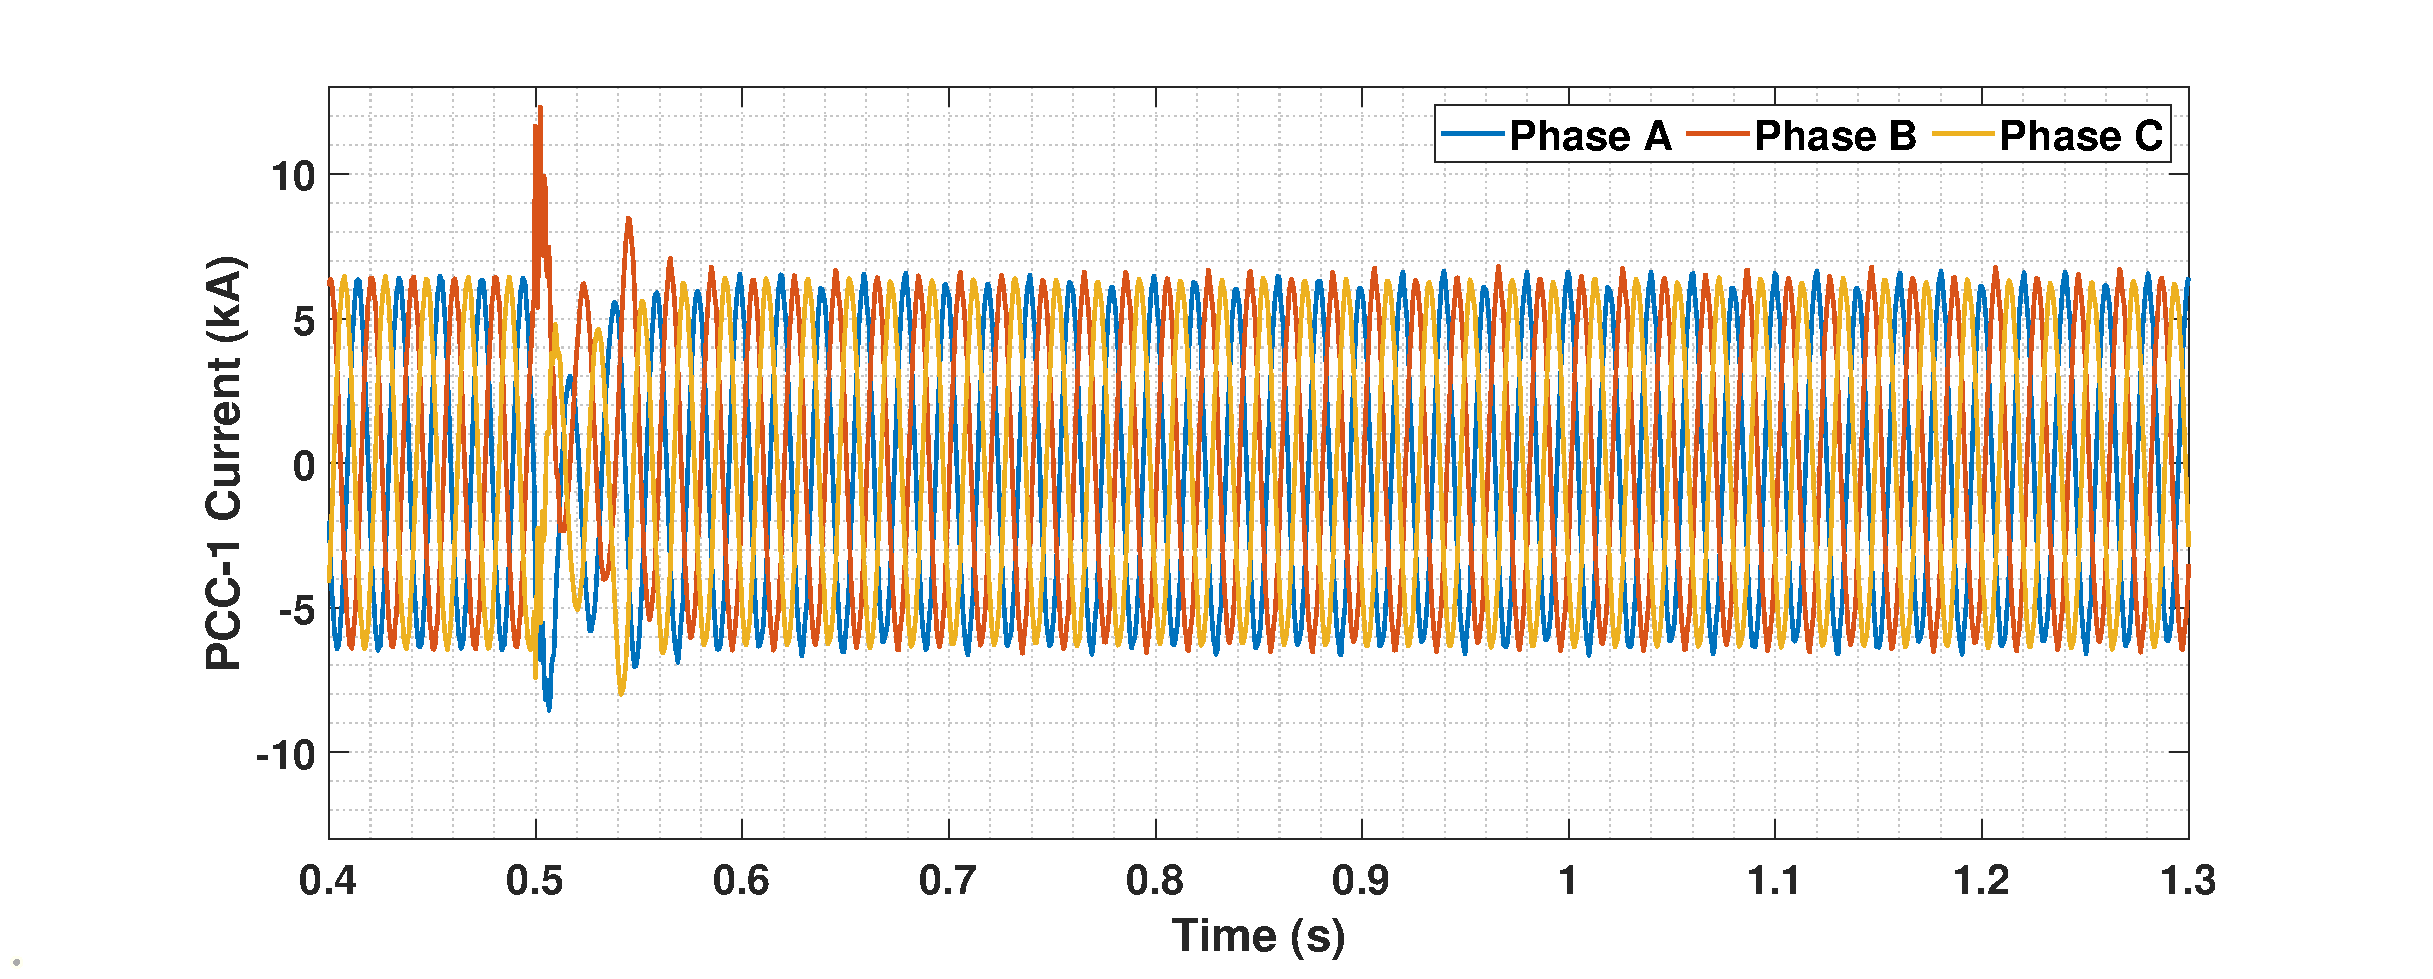
\includegraphics[height = 6.5cm,width = \textwidth]{Diagrams/Chapter_5/IABC_WT1_3phaseSC.eps}
    \caption{Currents in PCC-1 upon three-phase line to ground fault in the middle of cable-1}
    \label{WT1_currents_3phasefault}
\end{figure}


Voltages at \gls{PCC}-2, 3 and 4 have transients during the time of fault and are then stabilized to a slightly higher value than the pre-fault state to compensate for the loss of \gls{OWF}-1. This is due to the fast local voltage control in \gls{DVC} as seen for the case of disconnection of one \gls{OWF}. The post-fault voltage value is within the tolerance limit ($\pm$10 \% ), and this can be viewed from the graphs in Figure \ref{VACP_WT234_3phaseSC}. An important observation in the voltage graphs of \gls{OWF}s-2, 3 and 4 is the occurrence of spikes right after the circuit breaker CB-1a is opened, as can be seen in Figure \ref{VACP_WT234_3phaseSC}. 
There can be two reasons for such a phenomenon to occur. The first is that after the circuit breaker CB-1a is opened, reactive current injection still takes place (at 0.59 s in Figure \ref{IABC_WT2_3phaseSC} for \gls{PCC}-2) and this causes the voltage at the corresponding \gls{PCC} also to rise. Such a rise in voltage is not applicable in real-world \gls{OWF}s and is, therefore, a drawback due to the \gls{OWF} modelling. These spikes can be ignored as they do not represent the performance of the real hardware. The second reason could be due to two control strategies that provide the voltage reference in the network. It is seen that during the steady state and post-fault condition, the V/F control is dominant and provides the voltage reference in the network. However, during the time of the fault, \gls{DVC} in all \gls{OWF}s take the role of providing the voltage reference in the corresponding \gls{PCC}s as seen in \gls{PCC}-1 during the time of three-phase line to ground fault in cable-1. The sudden change back to the steady state condition after the fault is released could lead to discrepancies between the V/F mode and the \gls{DVC}. The conflict between these control strategies occur as to which control strategy provides the voltage reference right after the circuit breaker is open and hence this causes a spike in voltage at the \gls{PCC}s.

\begin{figure}[H]
%\centering
%\hspace*{-1.2cm}
\captionsetup{justification=centering}
    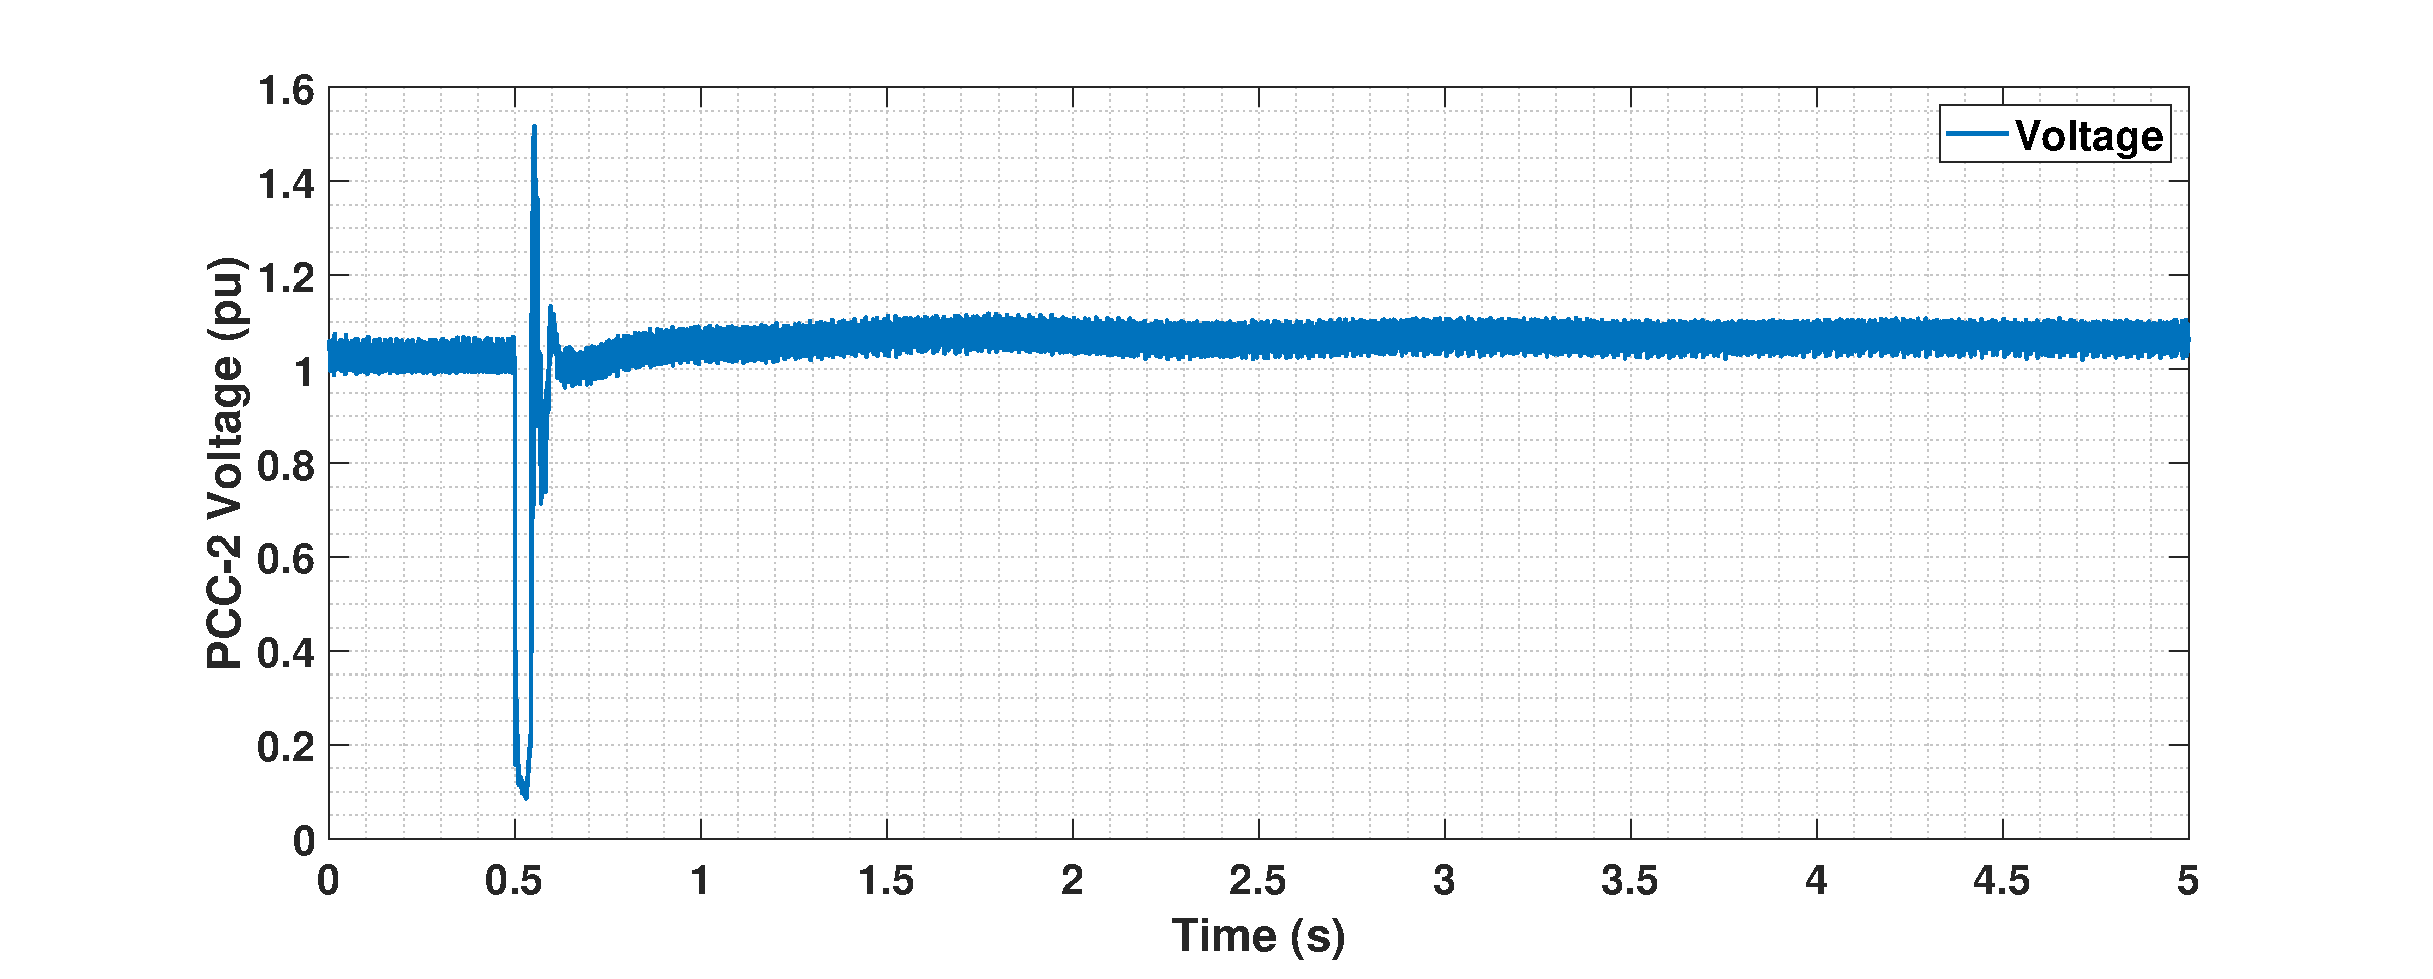
\includegraphics[height = 6.5cm,width = \textwidth]{Diagrams/Chapter_5/VACP_WT2_3phaseSC.eps}
    \caption{Voltage in p.u. at PCC-2 upon three-phase line to ground fault in the middle of cable-1}
    \label{VACP_WT234_3phaseSC}
\end{figure}

\begin{figure}[H]
%\centering
%\hspace*{-1.2cm}
\captionsetup{justification=centering}
    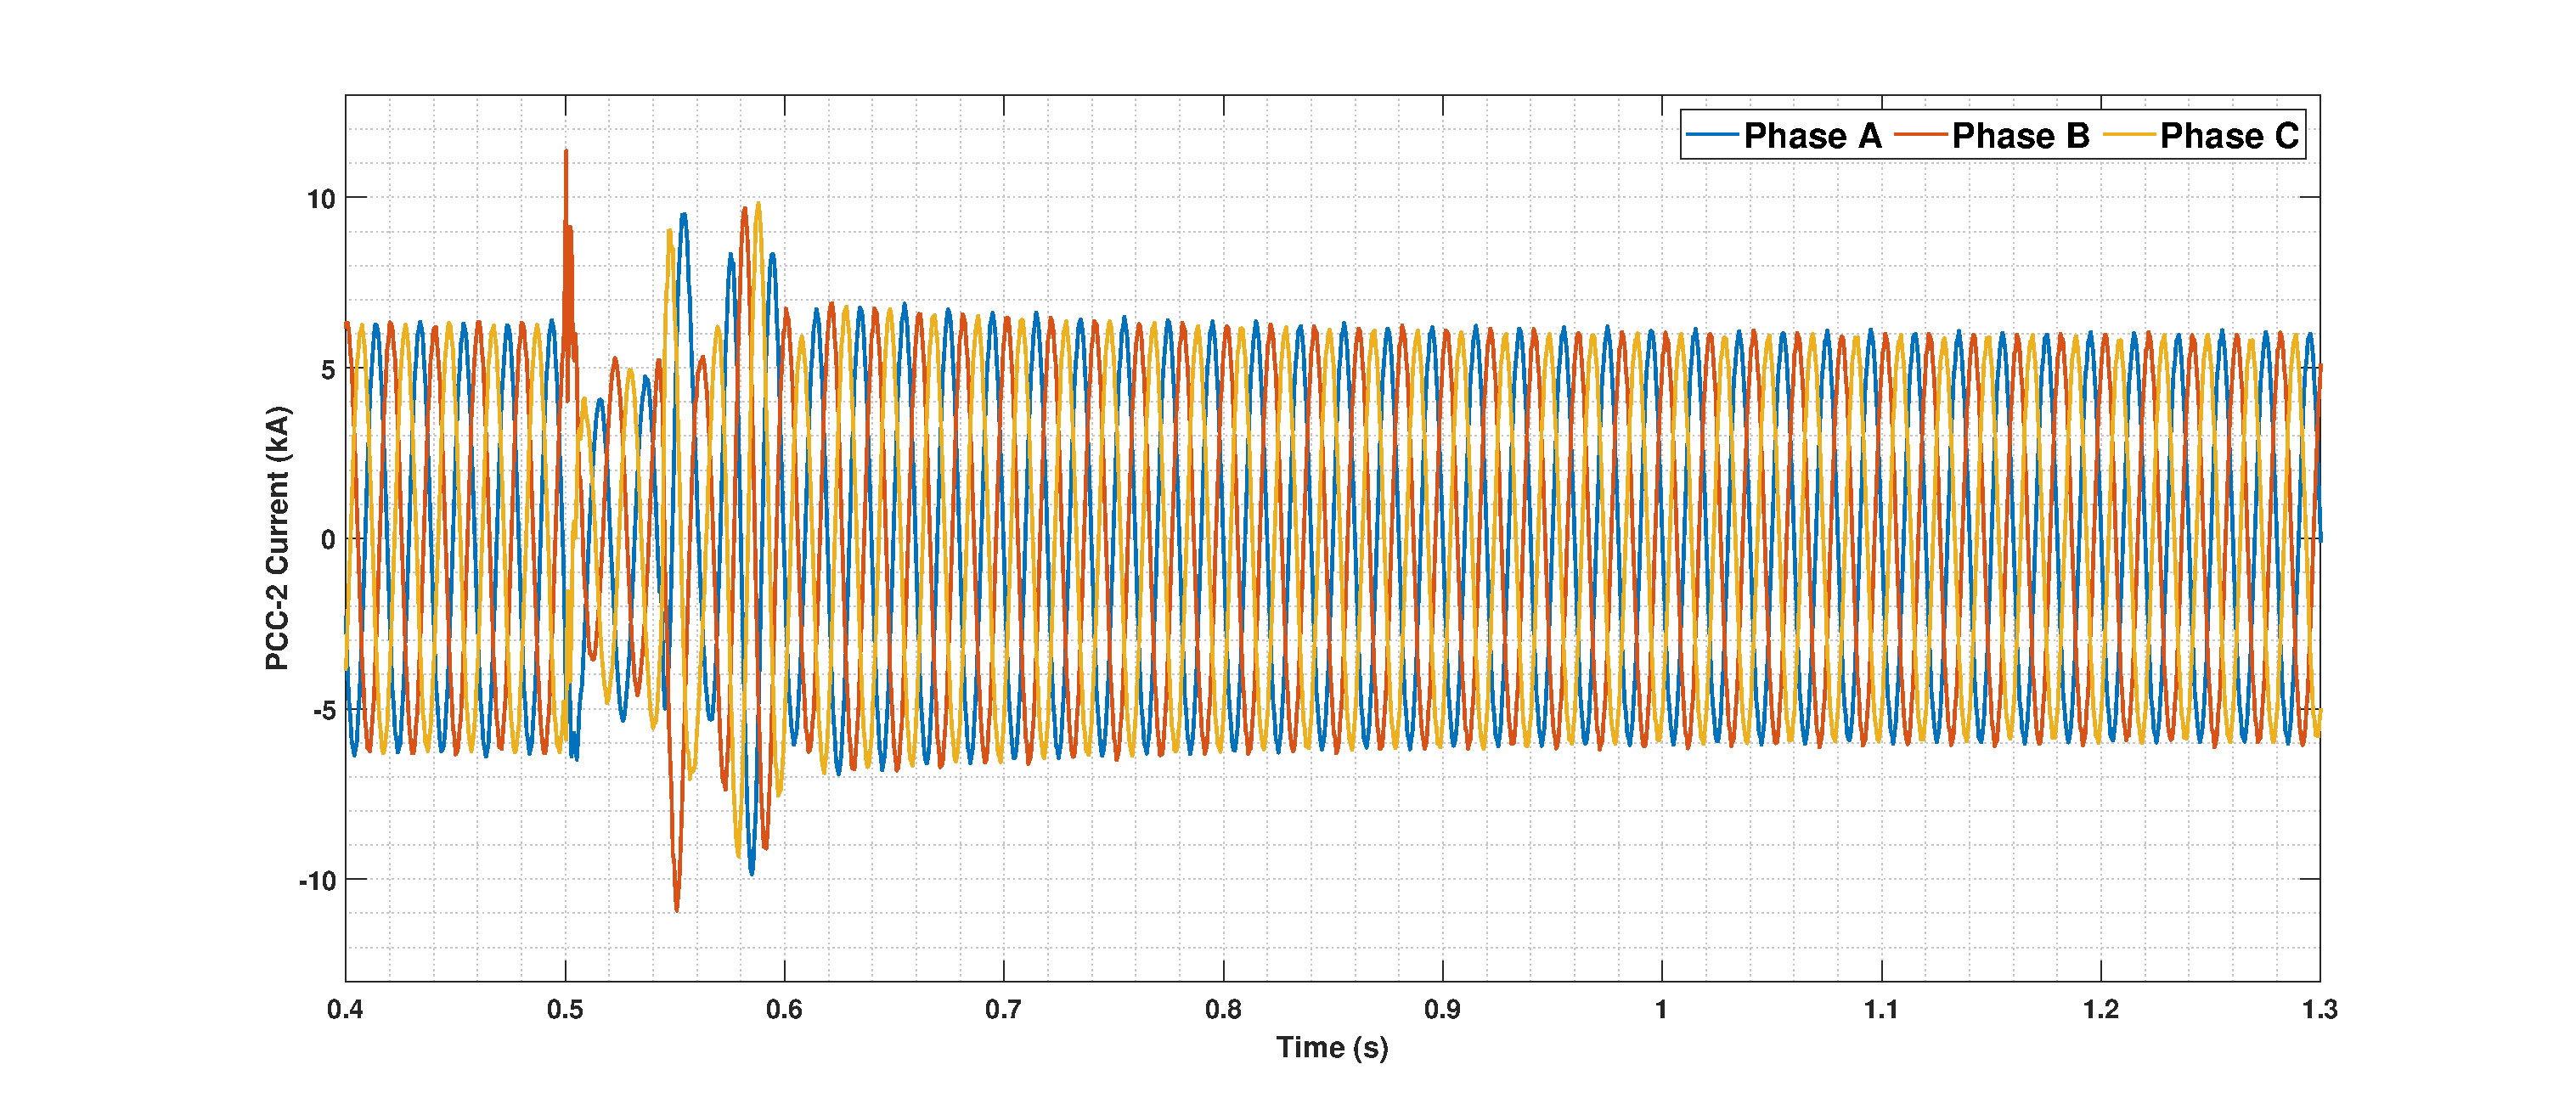
\includegraphics[height = 6.5cm,width = \textwidth]{Diagrams/Chapter_5/IABC_WT2_3phaseSC.eps}
    \caption{Currents in PCC-2 upon three-phase line to ground fault in the middle of cable-1}
    \label{IABC_WT2_3phaseSC}
\end{figure}

The currents from the \gls{OWF}s-2, 3 and 4 are the same in the post-fault region as the pre-fault condition (Figure \ref{IABC_WT2_3phaseSC} for \gls{PCC}-2) since the scaling factor for each \gls{OWF} is still the same. \gls{DVC} control in these \gls{OWF}s operate during the time of fault and limit the currents by controlling the voltages at corresponding \gls{PCC}s. Due to the increase in voltage in the post-fault period at the \gls{PCC}s-2, 3 and 4, the active power generated also will be higher from the \gls{OWF}s-2, 3 and 4 and it is reflected in the increase in active power in \gls{MMC}-2 as shown in Figure \ref{17_3phaseSC}. Another important observation is in the profile of transients in currents in \gls{PCC}s-2, 3 and 4 following the occurrence of the fault. As shown in Figure \ref{IABC_WT2_3phaseSC} for \gls{PCC}-2, the current is limited from 0.5 to 0.54 s during the time of fault. After the breaker has been operated at 0.542 s, the profile of currents (from 0.55 s to 0.6 s) is similar to that of the \gls{MMC}-2 (Figure \ref{fig:IABC_MMC_2_3phaseSC}). This is due to the re-synchronization to the grid by the \gls{PLL} in \gls{MMC}-2 control and the \gls{PLL} in \gls{DVC} of \gls{WG}-2, 3 and 4. 


%\vspace{-5.8mm}




In practice, if a three-phase fault occurs in a subsea cable, it is difficult that the fault clears on its own and would require human interference. During such critical islanding situations, the \gls{DVC} allows rated reactive current to flow to the fault location by controlling the \gls{GSC} voltage and thereby protecting the converters in the \gls{OWF} from high overcurrents. Based on the reference grid codes mentioned in \cite{mohseni_review_2012}, during steady state operation, the active current must be the priority, and during the time of the fault, the priority must be changed to reactive current. The major takeaway from this chapter is that the \gls{DVC} follows the reactive current injection requirement during the time of the fault, as shown from the currents in \gls{PCC}-1 in Figure \ref{IDQ_WT1_3phaseSC} even while working in coordination with other controls in the network. Current is limited to the rated current of the converter by the current limitation algorithm in \gls{DVC} without the requirement of any external controls. %Simultaneously, the currents in the other \gls{OWF}s are balanced as per the active power required in \gls{MMC}-2 as seen in Figure \ref{IDQ_WT2_3phaseSC}. 

%\vspace{-3mm}
\begin{figure}[H]
%\centering
%\hspace*{-1.2cm}
    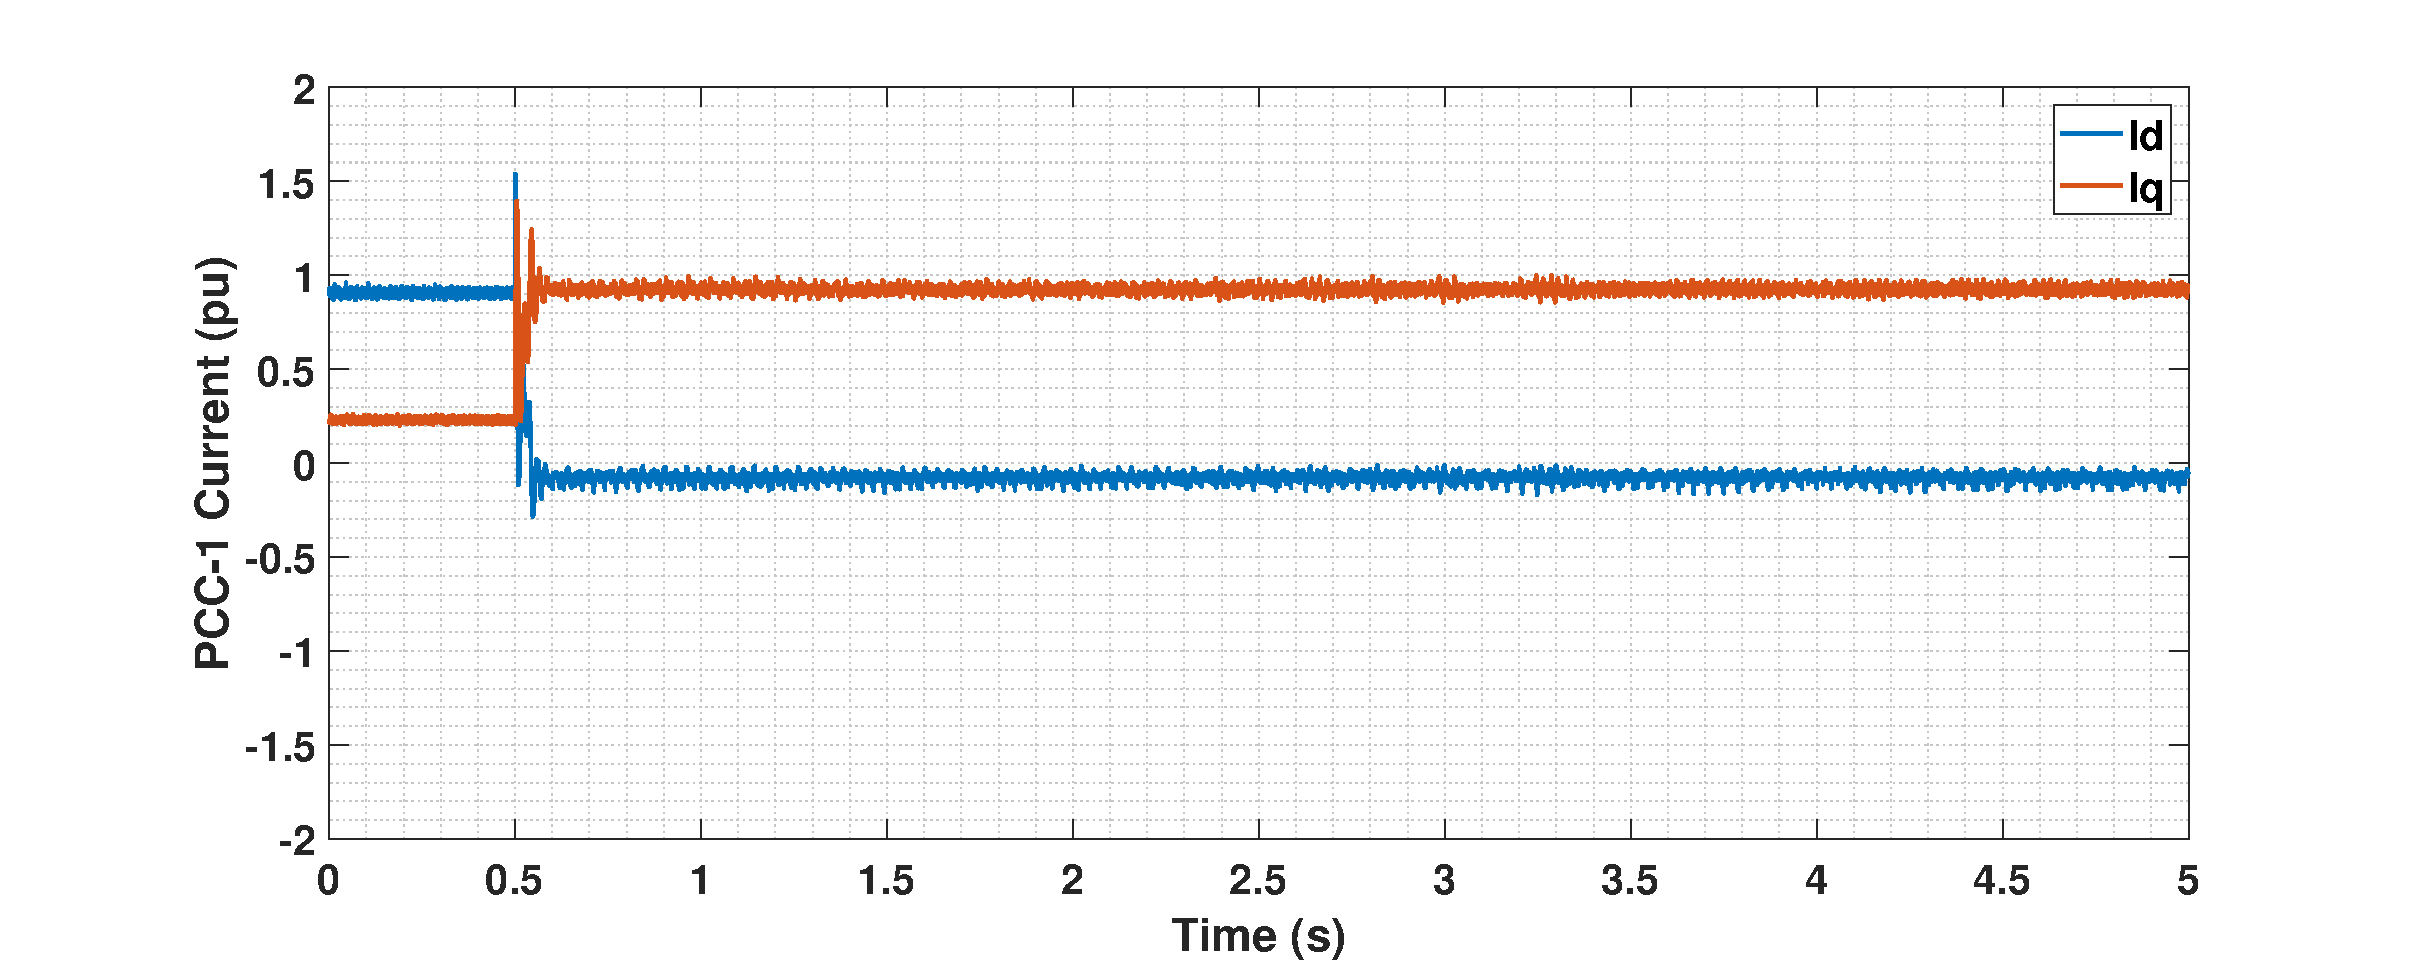
\includegraphics[height = 6.5cm,width = \textwidth]{Diagrams/Chapter_5/IDQ_WT1_3phaseSC_2.eps}
    \caption{Currents in d and q axes in PCC-1 upon three-phase line to ground fault in the middle of cable-1}
    \label{IDQ_WT1_3phaseSC}
\end{figure}


% \vspace{-5mm}
% \begin{figure}[H]
% %\centering
% %\hspace*{-1.2cm}
%     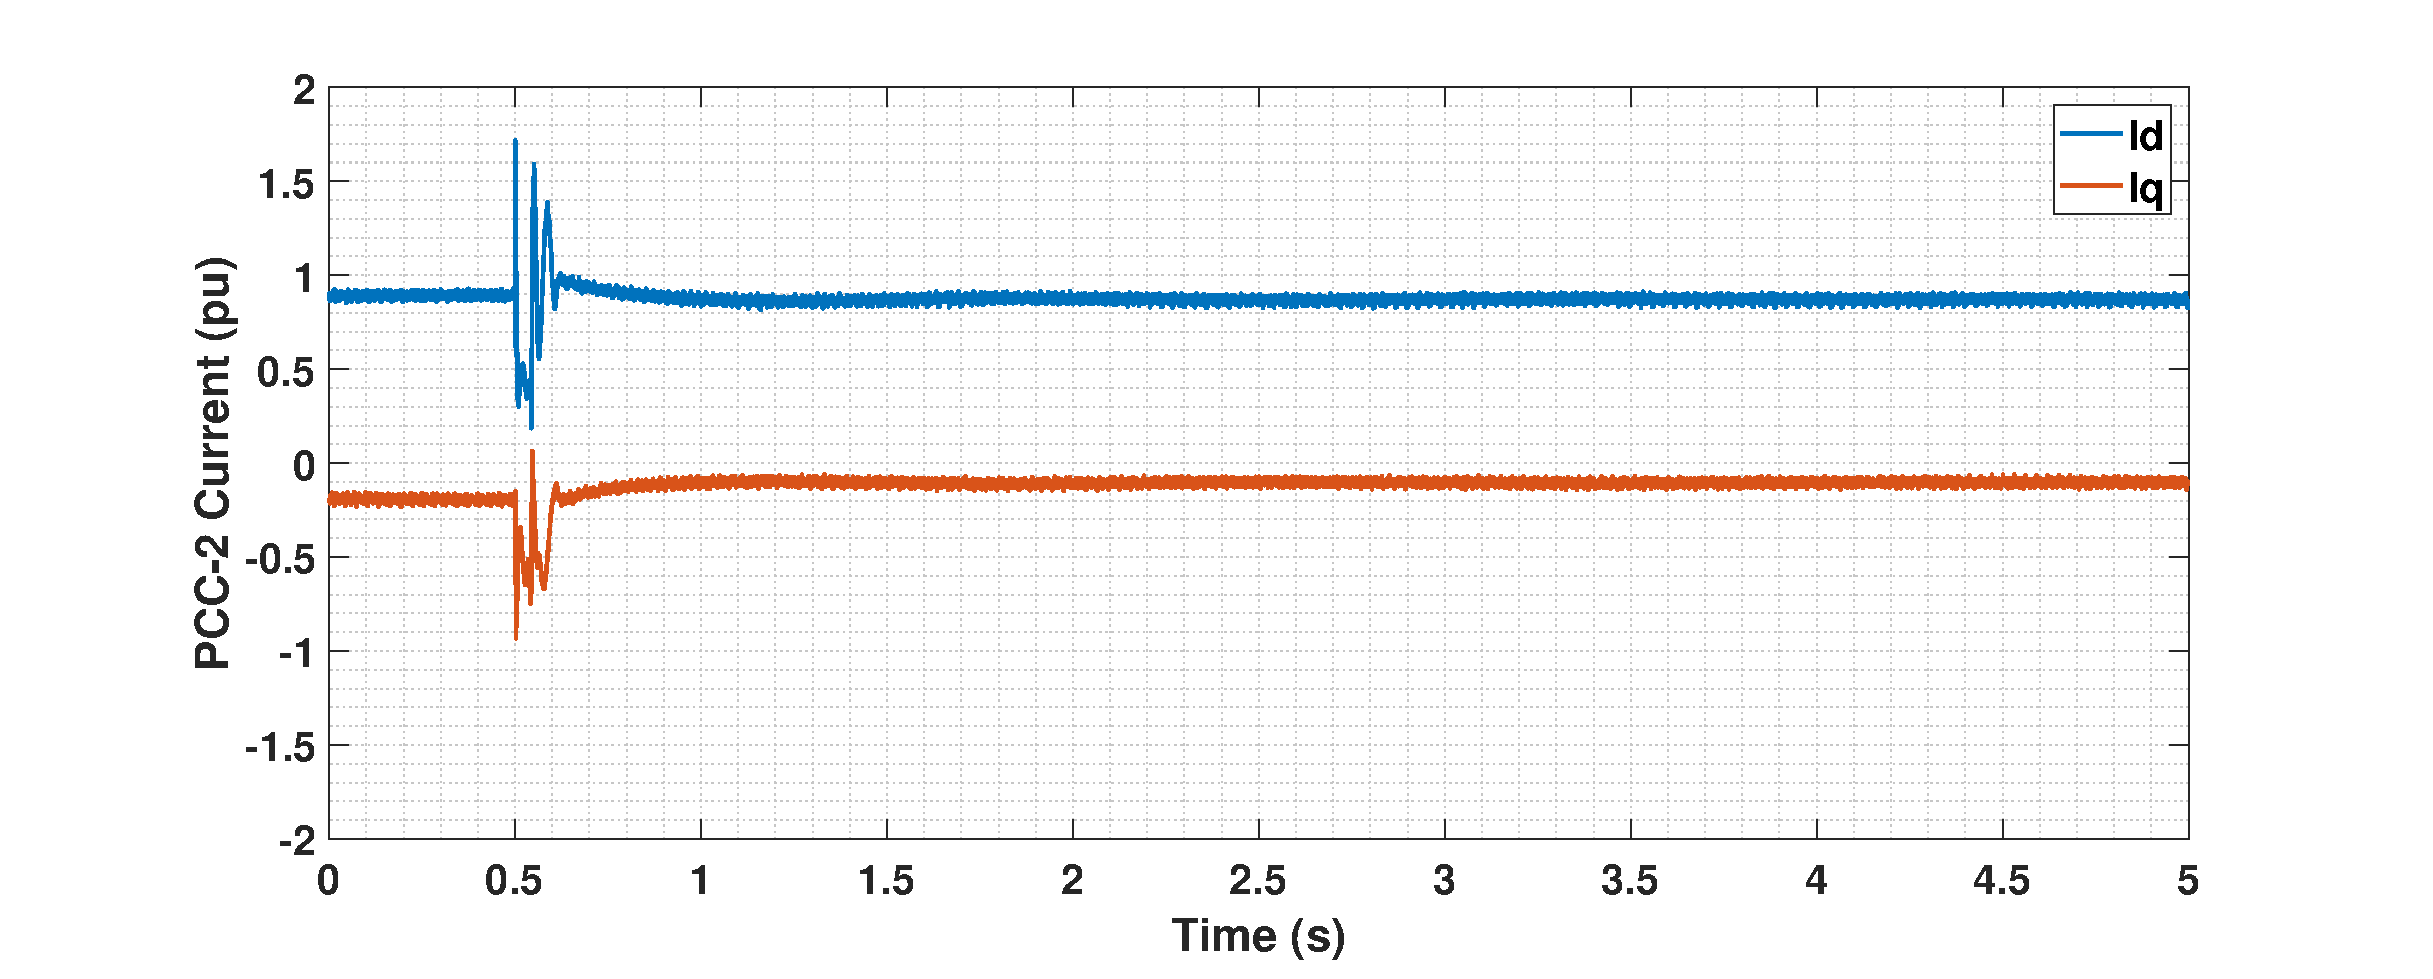
\includegraphics[height = 6cm,width = \textwidth]{Diagrams/Chapter_5/IDQ_WT2_3phaseSC.eps}
%     \caption{Currents in d and q axes in PCC-2 upon three-phase line to ground fault in the middle of cable-1}
%     \label{IDQ_WT2_3phaseSC}
% \end{figure}